%%%%%%%%%%%%%%%%%%%%%%%%%%%%%%%%%%%%%%%%%
% Short Sectioned Assignment LaTeX Template Version 1.0 (5/5/12)
% This template has been downloaded from: http://www.LaTeXTemplates.com
% Original author:  Frits Wenneker (http://www.howtotex.com)
% License: CC BY-NC-SA 3.0 (http://creativecommons.org/licenses/by-nc-sa/3.0/)
%%%%%%%%%%%%%%%%%%%%%%%%%%%%%%%%%%%%%%%%%

% \documentclass[paper=a4, fontsize=11pt]{scrartcl} % A4 paper and 11pt font size
\documentclass[11pt, a4paper]{book}
\usepackage[T1]{fontenc} % Use 8-bit encoding that has 256 glyphs
\usepackage[utf8]{inputenc}
\usepackage{fourier} % Use the Adobe Utopia font for the document - comment this line to return to the LaTeX default
\usepackage{listings} % para insertar código con formato similar al editor
\usepackage[spanish, es-tabla]{babel} % Selecciona el español para palabras introducidas automáticamente, p.ej. "septiembre" en la fecha y especifica que se use la palabra Tabla en vez de Cuadro
\usepackage{url} % ,href} %para incluir URLs e hipervínculos dentro del texto (aunque hay que instalar href)
\usepackage{graphics,graphicx, float} %para incluir imágenes y colocarlas
\usepackage[gen]{eurosym} %para incluir el símbolo del euro
\usepackage{cite} %para incluir citas del archivo <nombre>.bib
\usepackage{enumerate}
\usepackage{hyperref}
\usepackage{graphicx}
\usepackage{tabularx}
\usepackage{booktabs}
\usepackage{capt-of}
\usepackage{subcaption}

\usepackage{acronym}
\usepackage{pdflscape}
\usepackage{minted}

% jjramos
\usepackage[colorinlistoftodos,prependcaption,textsize=tiny]{todonotes}

\usepackage{xcolor}
\hypersetup{
	colorlinks=true,	% false: boxed links; true: colored links
	linkcolor=black,	% color of internal links
	urlcolor=cyan		% color of external links
}

\definecolor{LightGray}{gray}{0.9}

\definecolor{codegreen}{rgb}{0,0.6,0}
\definecolor{codegray}{rgb}{0.5,0.5,0.5}
\definecolor{codepurple}{rgb}{0.58,0,0.82}
\definecolor{backcolour}{rgb}{0.95,0.95,0.92}

\lstdefinestyle{mystyle}{
    backgroundcolor=\color{backcolour},   
    commentstyle=\color{codegreen},
    keywordstyle=\color{magenta},
    numberstyle=\tiny\color{codegray},
    stringstyle=\color{codepurple},
    basicstyle=\ttfamily\footnotesize,
    breakatwhitespace=false,         
    breaklines=true,                 
    captionpos=b,                    
    keepspaces=true,                 
    numbers=left,                    
    numbersep=5pt,                  
    showspaces=false,                
    showstringspaces=false,
    showtabs=false,                  
    tabsize=2
}

\lstset{style=mystyle}

\renewcommand{\familydefault}{\sfdefault}
\usepackage{fancyhdr} % Custom headers and footers
\pagestyle{fancyplain} % Makes all pages in the document conform to the custom headers and footers
\fancyhead[L]{} % Empty left header
\fancyhead[C]{} % Empty center header
% \fancyhead[R]{Pedro Miguel Parrilla Navarro} % My name
\fancyfoot[L]{} % Empty left footer
\fancyfoot[C]{} % Empty center footer
\fancyfoot[C]{\thepage} % Page numbering for right footer
%\renewcommand{\headrulewidth}{0pt} % Remove header underlines
\renewcommand{\footrulewidth}{0pt} % Remove footer underlines
\setlength{\headheight}{13.6pt} % Customize the height of the header

% \lstnewenvironment{listing}[1][]
%   {\lstset{#1}\pagebreak[0]}{\pagebreak[0]}

\usepackage{titlesec, blindtext, color}
\definecolor{gray75}{gray}{0.75}
\newcommand{\hsp}{\hspace{20pt}}
% \titleformat{\chapter}[hang]{\Huge\bfseries}{\thechapter\hsp\textcolor{gray75}{|}\hsp}{0pt}{\Huge\bfseries}
\setcounter{secnumdepth}{4}
% \usepackage[Lenny]{fncychap}

\makeatletter
\def\clearpage{%
  \ifvmode
    \ifnum \@dbltopnum =\m@ne
      \ifdim \pagetotal <\topskip
        \hbox{}
      \fi
    \fi
  \fi
  \newpage
  \thispagestyle{empty}
  \write\m@ne{}
  \vbox{}
  \penalty -\@Mi
}
\makeatother


\begin{document}

	% Plantilla portada UGR
	\begin{titlepage}
\newlength{\centeroffset}
\setlength{\centeroffset}{-0.5\oddsidemargin}
\addtolength{\centeroffset}{0.5\evensidemargin}
\thispagestyle{empty}

\noindent\hspace*{\centeroffset}\begin{minipage}{\textwidth}

\centering

\includegraphics[width=0.9\textwidth]{logos/nuevo_logo_ugr.png}\\[1.4cm]

\textsc{ \Large TRABAJO FIN DE GRADO\\[0.2cm]}
\textsc{ GRADO EN INGENIERÍA INFORMÁTICA}\\[1cm]

{\Huge\bfseries Diseño e implementación de una plataforma escalable para explotaciones agrarias \\}
\noindent\rule[-1ex]{\textwidth}{3pt}\\[3.5ex]
{\large\bfseries Utilizando ROS en el sector agrícola }
\end{minipage}

\vspace{1.5cm}
\noindent\hspace*{\centeroffset}
\begin{minipage}{\textwidth}
\centering

\textbf{Autor}\\ {Pedro Miguel Parrilla Navarro}\\[1ex]
\textbf{Directores}\\ {Juan Manuel López Soler}\\  {Juan José Ramos Muñoz}\\[2cm]

\includegraphics[width=0.3\textwidth]{logos/etsiit_logo.png}\\[0.1cm]
\textsc{Escuela Técnica Superior de Ingenierías Informática y de Telecomunicación}\\
\textsc{---}\\
Granada, Noviembre de 2021
\end{minipage}
\end{titlepage}

\newpage
\thispagestyle{empty}
\mbox{}
\newpage

	% Plantilla prefacio UGR
	\thispagestyle{empty}

\begin{center}
{\large\bfseries Diseño e implementación de una plataforma escalable para explotaciones agrarias }\\
\end{center}
\begin{center}
Pedro Miguel Parrilla Navarro\\
\end{center}
%\vspace{0.7cm}

\vspace{0.5cm}
\noindent{\textbf{Palabras clave}: \textit{Pub-Sub, agricultura, DDS, ROS, micro-ROS, Firebase, SQLite3, FastAPI, Angular}}
\vspace{0.7cm}

\noindent{\textbf{Resumen}}\\

En el sector agrícola está avanzando a pasos agigantados gracias a la inclusión de las diferentes tecnologías de comunicación, robóticas o todo lo relacionado con IoT. Las empresas están desarrollando e implementando sus plataformas en el mercado abarcando un gran número de clientes. En el documento se van a analizar los productos disponibles de manera genérica y tras esto realizar la propuesta de uno propio.

En este proyecto se va a diseñar e implementar una plataforma que utiliza comunicación un patrón Publicador-Suscriptor utilizando el conjunto de herramientas que proporciona ROS 2. Este trabaja sobre una capa DDS donde se implementa ese tipo de conexión. Tras la definición y conexión de los diferentes dispositivos, la información generada será almacenada en una base de datos para su posterior visualización en una interfaz web. Por último se realiza una evaluación de diferentes escenarios, añadiendo elementos de manera progresiva al hardware disponible.

\cleardoublepage

\begin{center}
	{\large\bfseries Design and implementation of a scalable platform for agricultural farms}\\
\end{center}
\begin{center}
	Pedro Miguel Parrilla Navarro\\
\end{center}
\vspace{0.5cm}
\noindent{\textbf{Keywords}: \textit{Pub-Sub, agriculture, DDS, ROS, micro-ROS, Firebase, SQLite3, FastAPI, Angular}}
\vspace{0.7cm}

\noindent{\textbf{Abstract}}\\
The agricultural sector is advancing very fast due to the use of different communication technologies, robotics and everything related to IoT. Companies are developing and implementing their platforms in the market covering a large number of customers. In this document we are going to analyse the available products in a generic way and after this we are going to make a proposal for one of our own.

In this project we are going to design and implement a platform that uses a Publisher-Subscriber communication pattern using the set of tools provided by ROS 2. This works on a DDS layer where this type of connection is implemented. After the definition and connection of the different devices, the information generated will be stored in a database for later visualisation in a web interface. Finally, an evaluation of different scenarios is carried out, adding elements progressively to the available hardware.

\cleardoublepage

\thispagestyle{empty}

\noindent\rule[-1ex]{\textwidth}{2pt}\\[4.5ex]

D. \textbf{Juan Manuel López Soler}, Profesor del Departamento de la Teoría de la Señal, Telemática y Comunicaciones, y D. \textbf{Juan José Ramos Muñoz}, Profesor del Departamento de la Teoría de la Señal, Telemática y Comunicaciones

\vspace{0.5cm}

\textbf{Informo:}

\vspace{0.5cm}

Que el presente trabajo, titulado \textit{\textbf{Diseño e implementación de una plataforma escalable para explotaciones agrarias}},
ha sido realizado bajo nuestra supervisión por \textbf{Pedro Miguel Parrilla Navarro}, y autorizo la defensa de dicho trabajo ante el tribunal
que corresponda.

\vspace{0.5cm}

Y para que conste, expiden y firman el presente informe en Granada a Junio de 2018.

\vspace{1cm}

\textbf{El/la director(a)/es: }

\vspace{5cm}

\noindent \textbf{Juan Manuel López Soler} \hspace{3.5cm} \textbf{Juan José Ramos Muñoz}

\chapter*{Agradecimientos}

Gracias a todos aquellos profesores que me han marcado y ayudado durante mi etapa de estudiante.

Gracias a mis amigos y compañeros de piso quienes me han acompañado durante esta etapa universitaria, tanto en las buenas, como en las malas.

Gracias a Alex por estar siempre ahí cuando necesito que me echen una mano.

Gracias a MJ por ayudarme y cuidarme durante estos meses de trabajo.

Gracias a mis padres y a mi hermano por haberme apoyado, orientado y hasta regañado en los momentos necesarios.

Y por último volver a destacar las gracias a mi padre, ya que sin él seguramente este proyecto no habría sido abordado de la misma manera.

	% Índice de contenidos
	\clearpage
	\tableofcontents

	% Índice de imágenes y tablas
	\clearpage
	\listoffigures
	
	\clearpage
	\lstlistoflistings
    
% % Listadode notas, jjramos
% 	\clearpage
%     \listoftodos[Notes]

% 	% Si hay suficientes se incluirá dicho índice
% 	\listoftables 
% 	\newpage

	% Introducción 
	\chapter{Introducción}

En este Trabajo Fin de Grado se va a diseñar, implementar y evaluar una plataforma basada en el paradigma Publicador-Suscriptor \cite{pub-sub-solutions} para un caso de uso en agricultura, utilizando el sistema \ac{ROS} \cite{ros2}. Esto es un conjunto de librerías y herramientas para creación de aplicaciones orientadas a creación de robots. En esta plataforma se identifican dispositivos muy variados divididos en dos grupos genéricos: sensores y actuadores. Además, se contará con un controlador que recopile la información y un gestor de la base de datos para almacenarlo. Por último se dispondrá de una interfaz web para la visualización de los datos más relevantes. A destacar, se utilizarán diferentes dispositivos hardware para realizar el despliegue y poder simular algunos elementos de un escenario real.

\section{Descripción del problema}

El problema viene en que los agricultores necesitan saber el estado del terreno o de la plantación durante el periodo de trabajo para obtener el máximo rendimiento posible sin pérdidas en la cosecha. Por ello en el caso de que las condiciones climatológicas cambien o se origine una plaga, tienen que responder a estas acciones de una forma u otra.

En algunos casos las propias máquinas ya lo tienen automatizado, pero hasta donde el autor conoce muy pocos tienen una interfaz o un tipo de respuesta que les confirme que este trabajo ha sido realizado y que los trabajadores puedan consultarlo desde sus casas. Por lo tanto la mayoría de ellos acaban acudiendo al terreno a comprobar este correcto funcionamiento.

\section{Motivación}

Esta temática de trabajo ha sido seleccionada ya que el sector de la tecnología aplicada en la agricultura está en auge. Han surgido empresas con productos muy variados estos últimos años, ofreciendo diferentes servicios según el interés de los clientes.

Como el crecimiento y las novedades en la tecnología aumentan de manera exponencial, algunos de estas instalaciones pueden quedarse obsoletas en poco tiempo según las herramientas utilizadas.

Por ello se ha escogido este tema, para proponer un proyecto el cual utiliza herramientas modernas para transmitir, automatizar y almacenar una serie de datos de manera digital, gracias a las \ac{TICs}.

\section{Objetivos}

Vamos a destacar en principio tres objetivos a cumplir, y tras esto una breve explicación de ellos.

En principio, se va a realizar un diseño que permita monitorizar y automatizar procedimientos en una explotación agrícola.

El siguiente es la posibilidad añadir nuevos tipos de sensores o actuadores, sin afectar poco o nada a los demás componentes de este diseño. Un ejemplo sería un robot para transporte o un dron que realice un recorrido mientras vierte un producto.

Por último almacenar estos datos, para luego poder tratarlos y procesarlos para su visualización. Por destacar, en un trabajo futuro podrían ser utilizados para el entrenamiento de alguna \ac{IA}.

\section{Estructura del documento}

En el capítulo 2 se va a abordar el estado del sector a tratar, las tecnologías aplicadas por las diferentes empresas y un listado de las diferentes herramientas posibles a utilizar en el proyecto.

En el capítulo 3 se habla sobre la metodología aplicada, como ha sido llevado a cabo el proyecto con su respectivo diagrama de Gantt y un esquema del presupuesto total.

El capítulo 4 analiza el proyecto, que es necesario desarrollar y en qué partes se va a dividir.

En el capítulo 5 se explica la implementación realizada del proyecto, siguiendo el orden y estructura establecida en la parte del análisis.

El capítulo 6 presenta diferentes escenarios evaluados, describiendo que componentes se utilizan y midiendo la memoria al ejecutar ciertos procesos.

Por último, en el capítulo 7 se hace una reflexión sobre todo lo aprendido y proyectado en este trabajo, obteniendo conclusiones sobre ello. Tras esto se finaliza destacando algunas tareas a realizar en el futuro.

	% Estado del arte
	% 	1. Crítica al estado del arte
	% 	2. Propuesta
	\chapter{Estado del arte}

 En este capítulo se revisarán la literatura relacionada con la Agricultura inteligente, así como las plataformas comerciales existentes.
%Si queremos ponernos en situación respecto a este trabajo y a las empresas, primero tenemos que explicar un concepto que surgió en los últimos años, la Agricultura 4.0 o Agricultura Inteligente.

% \section{La revolución verde}

% \section{Internet of Food \& Farm}

\section{Agricultura inteligente}
% Puedo hacer subsecciones de la lista y extenderlo más del articulo incluido en el doc%
%https://agrospray.com.ar/blog/agricultura-4-0/%



La agricultura inteligente \cite{agricultura-40}, o agricultura 4.0 se basa en la recopilación y análisis de datos sobre el campo, con el objetivo de mejorar la calidad de los cultivos y reducir las consecuencias en el medio ambiente.

Esto es posible con el uso de las nuevas tecnologías. Los diferentes robots, sensores, software, etc, son capaces de realizar tareas agrícolas en menos tiempo que el ser humano y con mejor resultados.

Ejemplos de tecnología utilizada en la agricultura:

\begin{itemize}
    \item \textbf{Sensorización ambiental}, referente al uso de sensores, obteniendo la información en tiempo real para optimizar mejor los recursos.
    \item \textbf{Uso de drones y teledetección}, con el objetivo de tomar fotos para analizar el estado, o incluso pulverizar un producto en cultivos.
    \item \textbf{Sistemas predictivos}, permitiendo la anticipación a las diferentes condiciones meteorológicas en las próximas horas o días.
    \item \textbf{Inteligencia artificial}, para tomar decisiones o realizar recomendaciones en base a los datos procesados.
    
\end{itemize}

Aparte de estos puntos, podemos destacar unos de los temas tocados en este proyecto, la robotización.

\subsection{Robots en el sector}


En \cite{revista-agraria} hay un artículo donde se comenta que los desarrolladores actualmente están trabajando en máquinas autónomas capaces de realizar tareas como las siguientes:

\begin{itemize}
    \item \textbf{Desbrozar}. Eliminar las malas hierbas mediante el reconocimiento de imagen con una cámara y expulsar dosis de herbicida según la mala hierba y el tamaño
    \item \textbf{Recogedor}. Realizar una recolecta del cultivo mediante la utilización de brazos robóticos, analizando la madurez de este.
    \item \textbf{Abonador}. Analiza el tamaño y color de las hojas de cada planta, aplicando una dosis de fertilizante según la necesidad de este.
\end{itemize}

Todas estas máquinas se podrían comunicar entre ellas, siendo controladas por un operador o trabajando de manera autónoma con ciertos horarios. Estas podrían ser utilizadas en los siguientes escenarios que se explicarán a lo largo del documento.

\section{Sistemas utilizados en la industria}

Esta parte ha sido una de las más complicadas de escribir, ya que no es fácil saber que tecnologías utilizan estas empresas debido a que las explicaciones realizadas en sus respectivas páginas web son muy genéricas del estilo: \textit{Consulta tus datos en tiempo real desde cualquier dispositivo.}

Como se ha visto en el anterior apartado, la mayoría de empresas tienen en común: \textbf{sensores} y \textbf{actuadores}, los cuales se van a agrupar de ahora en adelante como \textbf{nodos}.

Estos son la base del sistema, ya que son los \textbf{productores} de los datos a tratar, y de los cuales se obtiene la mayoría de la información. A continuación voy a realizar una lista de los algunos tipos que se deberían contemplar en el diseño, pudiendo ser estos aún más según las necesidades:

\begin{itemize}
    \item Temperatura del suelo, para ver el estado de la planta
    \item Humedad, tanto fuera como dentro del invernadero
    \item Estado hídrico del cultivo, para controlar los patrones de riego
    \item Velocidad del Viento
    \item Dirección del viento
\end{itemize}

Estos productores sirven para que los actuadores hagan ciertas funciones. Pero además hay otros actuadores que quizás no necesitan la información de estos sensores como un robot de transporte, brazo robot de recolecta, o algo más factible como los drones para realización de fotografías. Algunos actuadores que si utilizan la información de los productores son:

\begin{itemize}
    \item \textbf{Ventanas}, para transpirar y cambiar el aire de dentro
    \item \textbf{Calefactores}, para aumentar la temperatura
    \item \textbf{Humidificadores}, necesario en climas secos
    \item \textbf{Tuberías para riego}, permitiendo la circulación del agua
    \item \textbf{Pantallas térmicas}, con el objetivo de mantener fresco el terreno en días de mucho calor
    \item \textbf{Destratificadores}, ciclando el aire del interior, ya que el aire frío suele quedarse a nivel del suelo y el caliente tiende a subir.
\end{itemize}

En el siguiente conjunto de figuras \ref{fig:imagenes-actuadores} hay mostrados algunos de los actuadores menciondos

\begin{figure}[h]
\begin{subfigure}{\textwidth}
\centering
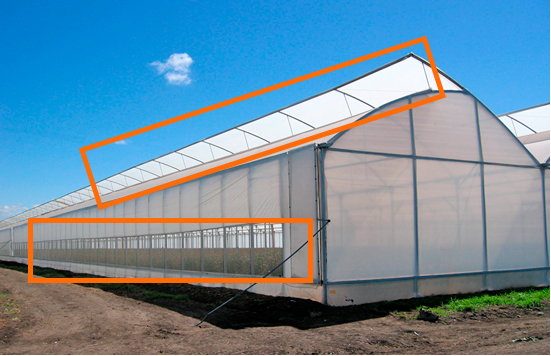
\includegraphics[width=0.9\textwidth, height=6cm]{img/03-Ventana.png}
%https://www.agroprecios.com/noticias.php/noticias/3371-mas-del-90-de-los-agricultores-de-almeria-controlan-manualmente-las-ventanas-del-invernadero?len=1
\caption{Ventanas (Imagen de la web de agroprecios)}
\label{fig:ventanas}
\end{subfigure}
\begin{subfigure}{\textwidth}
\centering
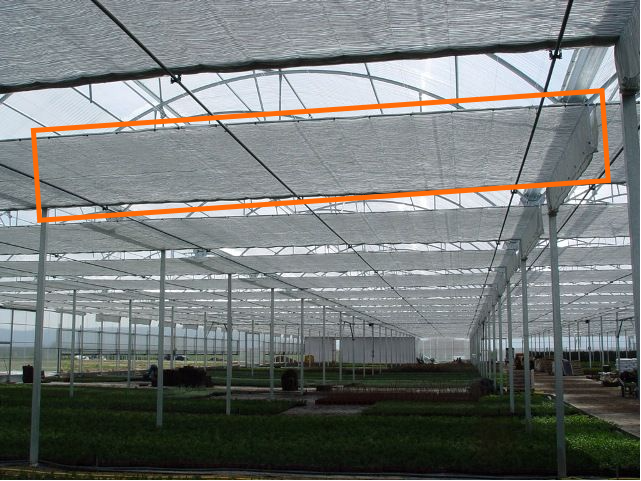
\includegraphics[width=0.9\textwidth, height=6cm]{img/03-PantallaTermica.png}
% https://fertri.com/accesorios-y-componentes/pantallas-termicas/
\caption{Pantallas térmicas (Imagen de la web fertri.com \cite{fertri})}
\label{fig:pantallas-termicas}
\end{subfigure}

\begin{subfigure}{\textwidth}
\centering
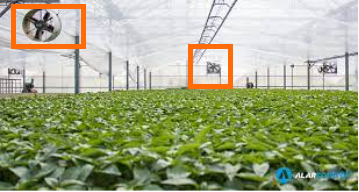
\includegraphics[width=0.9\textwidth, height=6cm]{img/03-Destratificador.png}
% https://fertri.com/accesorios-y-componentes/pantallas-termicas/
\caption{Destratificador (Imagen de la web de Alarcontrol \cite{alarcontrol-sl})}
\label{fig:destratificador}
\end{subfigure}

\caption{Imágenes de diferentes actuadores}
\label{fig:imagenes-actuadores}

\end{figure}

\clearpage

Por lo tanto, tras estudiar los diferentes productos desplegados por las empresas que las empresas utilizan, el autor de este trabajo propone dividir las soluciones actuales en dos grupos: \textbf{centralizadas} o \textbf{descentralizadas}.

% Aclaración de centralizado y descentralizado

\subsection{Despliegues centralizados}

En este caso, todo está conectado a un nodo que orquesta toda la plataforma.
Un ejemplo de empresa que utiliza este despliegue es Alarcontrol S.L. \cite{alarcontrol-sl}. 

La figura \ref{fig:despliegue_centralizado} nos da una idea de cómo es esta implementación. Esta consta de un panel central, donde un dispositivo gestiona todas las tareas, recopilando los datos de los diferentes sensores colocados en puntos estratégicos del terreno y conectados cada uno mediante un cable a la placa central.

\begin{center}
    \centering
    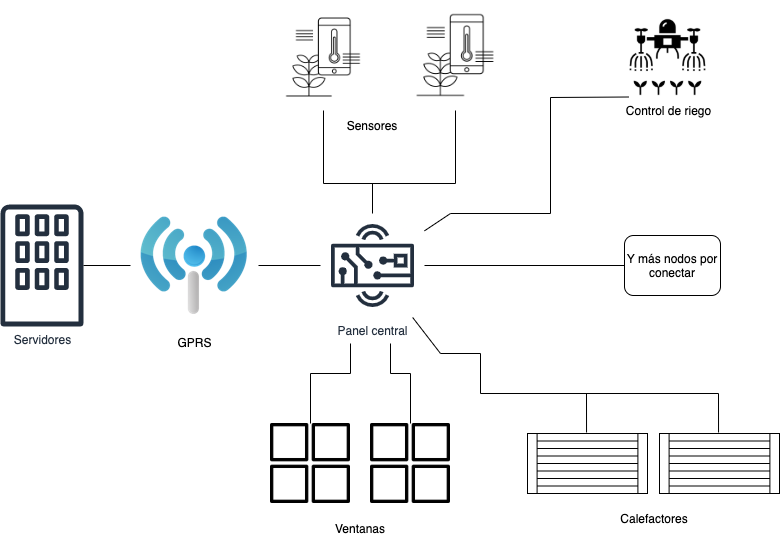
\includegraphics[width=\textwidth]{img/02-DespliegueCentralizado.png}
    \captionof{figure}{Despliegue centralizado (Elaboración propia)}
    \label{fig:despliegue_centralizado}
\end{center}

En el panel central se podrían encontrar diferentes botones para diversas acciones, además de una réplica de este dentro del invernadero para gestionar otros actuadores más cercanos, como ventanas o calefactores.

Por último tiene conexión \ac{GPRS}%, que es lo que venimos a conocer como cobertura móvil
. 
Esta la utiliza para transmitir los datos a un servidor central y que el usuario desde el móvil pueda visualizarlos.


Una posible desventaja de este servicio es la disponibilidad, ya que en el caso de que falle el %ese mencionado anteriormente 
gestor central no se podría disponer de ningún dato generado ni de los actuadores. Esto es debido a que no hay un sistema de respaldo, por lo tanto por muchas pruebas que se le hayan realizado, podría fallar.

\subsection{Empresas con despliegues descentralizados}

A diferencia del anterior, al ser descentralizado, no todo es gestionado por un único dispositivo, si no que podemos encontrar varios. Ejemplos de empresas que utilizan este diseño son Nazaríes \cite{nazaries} y Hortisys \cite{hortisys}.

Este sistema distribuye las tareas en más nodos, que poseen conectores genéricos para enchufar diferentes dispositivos, en función requiera el usuario. En el caso de la empresa Nazaríes, los nombra como \textit{Dataloggers}, que viene a ser recopilador de datos. Un ejemplo de este dispositivo lo podemos visualizar en la siguiente figura:

\begin{center}
    \centering
    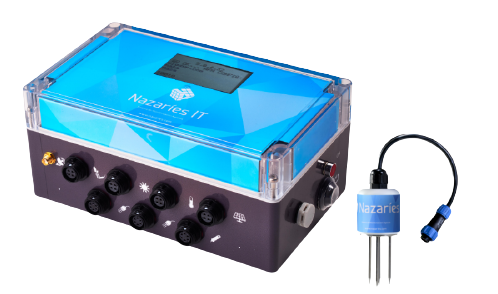
\includegraphics[width=0.5\textwidth]{img/03-Datalogger-Nazaries.png}
    \captionof{figure}{Datalogger GPRS junto a un sensor (Imagen de Nazaries \cite{nazaries})}
    \label{fig:datalogger-nazaries}
\end{center}

Como podemos observar, en el pie de la figura se hace referencia de GPRS. Esto es debido a que hay diferentes tipos de recopiladores de información según su conexión o visualización de datos: bluetooth, sigfox \cite{sigfox} o mostrados en un terminal.

% Añadir descripciones de bluetooth, sigfox, terminal?

Esto significa que trabaja de manera similar al despliegue centralizado, lo único que divide la carga, ya que diferentes nodos se encargan de recopilar esta información.

Pero esto también plantea un problema, y es que si uno de esos nodos se rompe, todos los datos que recopilaba no pueden ser visualizados.

Este supuesto fallo sería menos grave que en el caso anterior, ya que en el otro la plataforma entera dejaría de funcionar, y en este conlleva la pérdida de información del número de sensores conectados a este \textit{datalogger}.

\section{Tecnologías para publicación suscripción} \label{tecnologias_a_usar}

En el articulo de la bibliografía \textit{Meeting iot platforms re-quirements with open pub/sub solutions} \cite{pub-sub-solutions}, se define el patrón pub-sub como un \ac{MoM} que proporciona una comunicación distribuida, asíncrona entre productores y consumidores de mensajes. Este patrón presenta tres tipos principales de desacoplamiento que lo hacen especialmente adecuado para los despliegues de \ac{IoT} a gran escala:

\begin{itemize}
    \item Los productores de mensajes (publicadores) y los consumidores (suscriptores) están desacoplados en el tiempo, es decir, no tienen que estar conectados al mismo tiempo.
    \item Los mensajes no se dirigen a un consumidor en específico, si no a una dirección simbólica (canal, tópico)
    \item La mensajería es asíncrona y no se bloquea.
\end{itemize}

Uno de los elementos fundamentales de los sistemas pub/sub es la correspondencia entre productores y suscriptores, que puede basarse en distintos tipos de filtrado, principalmente de temas o contenidos. Este filtrado suele ser realizado por múltiples intermediarios de mensajes dedicados.

Tras la introducción de este sistema, se va a realizar una breve descripción de algunas tecnologías que lo aplican y cuál ha sido escogida para este proyecto.

\subsection{RabbitMQ}

RabbitMQ \cite{rabbitmq} es un software message-broker (negociador de mensajes) originalmente implementado con el protocolo \ac{AMQP}, con soporte a otros protocolos como por ejemplo \ac{STOMP} y \ac{MQTT}. Tiene la ventaja de que es independiente al lenguaje utilizado, y puede ser desplegado en .NET, Python, PHP, Ruby, etc.

Esta tecnología empezó como sistema de colas, por ello la parte de MQ en el nombre. Debido a esto, la implementación que realiza pub-sub está construida sobre este sistema. Esto puede ser que no sea lo más eficiente respecto a otra alternativa que su diseño si sea basado en el modelo de pub-sub. Además utiliza brokers (intermediarios entre pub-sub), haciendo que la conexión no sea directa y surja otro punto de posible fallo.

\subsection{Apache Kafka}

Kafka \cite{kafka} es un sistema de mensajería tipo pub-sub, escrito en lenguaje Scala, siendo escalable, duradero y tolerante a fallos. Es utilizado por empresas como Linkedin, Yahoo, Twitter y otras.

Su principal uso destaca en el análisis a tiempo real, pero se puede utilizar para supervisión, reproducción de mensajes, agregación de registros, recuperación de errores y el seguimiento de la actividad de un sitio web.

Pero para uso en IoT donde los dispositivos están conectados a un centro de datos o a la nube, Kafka no es idónea ya que necesita bastante configuración. Además hay una serie de puntos que no la hacen idonea para este entorno:
\begin{itemize}
    \item No soporta una enorme cantidad de tópicos
    \item Los brokers necesitan estar directamente direccionados por los clientes
    \item Algunas de las claves de las funcionalidades de IoT no están presentadas en Kafka, como por ejemplo \textit{keep alive}. Esta hace referencia al historial de datos a mantener en la red.
    \item Es necesario una conexión estable TCP, no muy presente en estos entornos, haciendo que los dispositivos gasten recursos en la reconexión.
\end{itemize}

\subsection{ROS2}

ROS2 \cite{ros2} es un conjunto de herramientas software utilizadas principalmente para la creación de estos robots. Empresas como BMW de automoción o la NASA utilizan ROS en algunos de sus proyecto. Por destacar, es utilizado en el Robonaut 2 \cite{robonaut}.

Las características principales que surgieron tras su desarrollo fueron:

\begin{itemize}
    \item Sistemas en tiempo real, para diferentes tratamientos de datos
    \item Equipos de múltiples robots, pudiendo comunicarse entre ellos para diferentes tareas
    \item Para conexiones no ideales, es decir, gestionando perdidas o delay de una red WiFi de poca calidad
\end{itemize}


Por defecto, ROS2 utiliza \ac{DDS} \cite{dds-omg} como middleware para la comunicación. 
DDS está orientado a usarse en computación distribuida implementando el patrón de esta sección, publicador-subscriptor. Permite el manejo de los mensajes de manera transparente sin la necesidad de la intervención del usuario, incluyendo algunas funciones como quien debería recibir el mensaje, donde están situados los consumidores o que pasaría si el mensaje no pudiese ser enviado. Además DDS soporta diferentes lenguajes como C, C++, Java o Python gracias a la \ac{APIs} disponibles. Esto permite que diferentes dispositivos, con sistemas operativos o lenguajes distintos puedan comunicarse. Esto viene a ser conocido como interoperabilidad.

\begin{center}
    \centering
    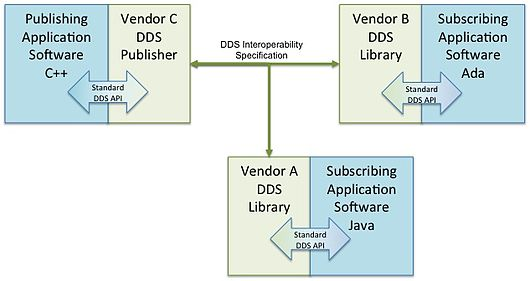
\includegraphics[width=0.5\textwidth]{img/03-DDS-Interoperability.jpeg}
    \captionof{figure}{OMG DDS interoperabilidad}
    \label{fig:dds-wiki}
\end{center}

El escenario mostrado en la figura \ref{fig:dds-wiki} se puede obtener del artículo \cite{dds-omg}. En el se explica la interoperabilidad del protocolo utilizado para la conexión de los diferentes dispositivos.

Tras explicar algunos conceptos y funcionalidades sobre DDS, caracterizar que no existen brokers en algunas de sus implementaciones, ya que utiliza un protocolo multicast basado en descubrimiento de dispositivos (intermediarios entre pub-sub). Además simplifica el despliegue, minimiza la latencia, maximiza la escalabilidad y aumenta la fiablilidad. Por tanto es idóneo para aplicaciones IoT que requieren de una arquitectura duradera y fiable.

Respecto a ROS 2, utiliza un middleware para ser independiente a la implementación de DDS utilizada, además de ofrecer una API para los diferentes lenguajes de programación soportados. Esta información se puede visualizar en la siguiente imagen:


\begin{center}
    \centering
    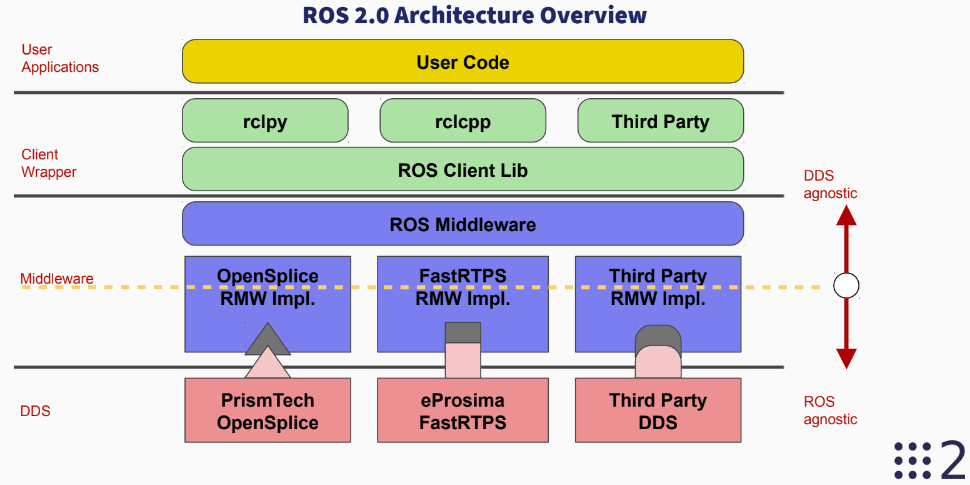
\includegraphics[width=\textwidth]{img/03-ROS2-Middleware.png}
    \captionof{figure}{Capas disponibles con ROS 2}
    \label{fig:ros-layers}
\end{center}

En la figura \ref{fig:ros-layers} se puede observar las capas de la API que ofrece ROS 2.

Por último, ROS2 es compatible con múltiples implementaciones de DDS, como de eProsima's Fast DDS \cite{fastdds}, RTI's Connext DDS \cite{connextdds} y Eclipse Cyclone DDS \cite{cyclonedds}. Por defecto, ROS2 utiliza el producto de eProxima's.

Cabe destacar que para poder utilizar ROS en microcontroladores, es necesario el uso de microROS. Este se diferencia de que la implementación es realizada en C/C++, además que deberá situarse en una capa por encima que actúe como sistema operativo, como \ac{FreeRTOS}.

El diagrama de comunicación y de capas se puede visualizar en la siguiente imagen:

\begin{center}
    \centering
    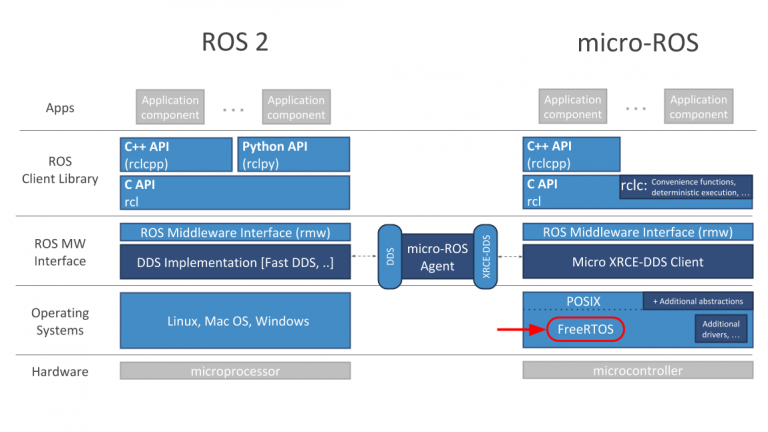
\includegraphics[width=\textwidth]{img/02-micro-ros.png}
    \captionof{figure}{Comparación estructura ROS2 y microROS}
    \label{fig:ros2-microros}
\end{center}

Como se puede observar en \ref{fig:ros2-microros}, en el centro esta situado una figura que pone micro-ROS Agent. Este es el encargado de comunicar la parte de DDS (la parte del middleware de ROS) generada por el microcontrolador con las diferentes implementaciones de DDS que existan en la red.
	
	\chapter{Planificación}

En este capítulo se describe la metodología utilizada en el proyecto, cómo se van a gestionar las tareas a lo largo del tiempo con un diagrama de Gantt y tras esto la evaluación del coste de todo el material y trabajo a realizar.

Por último se planteará otro diagrama de Gantt donde se muestran las franjas de las actividades de cómo han ocurrido de manera real y si son próximas a las estimadas.

\section{Metodología utilizada}

Respecto a la metodología utilizada va a ser una variante de Scrum, ya que se iran  realizando tareas (sprints) que serán evaluadas en periodos semanales por el tutor. Estas tienen el objetivo de ir expandiendo el producto poco a poco, y se puedan visualizar los diferentes requisitos aplicados. 

Tras la finalización de cada tareas, hay una reunión donde se discute la tarea realizada, y en el caso de cómo ha ido su desarrollo, se volverá a revisar o se avanzará a la siguiente tarea, pudiendo ir modificando la orientación del proyecto.

Además se ha hecho uso de un repositorio Github para realizar un control del siguiente proyecto. El link es el siguiente: \href{https://github.com/pparrilla/ROS2_TFG}{github.com/pparrilla/ROS2\_TFG}

\section{Temporización}

Para el registro de horas se va a utilizar la aplicación Clockify \cite{clockify}. Esta permite ir creando tareas diarias con un nombre, un tag referente a que grupo pertenece e indicar el proyecto. Este registro de horas es necesario para ir realizando comparaciones con el tiempo que se ha estimado para cada tarea.

A fecha de la planificación del proyecto se estima que con las horas llevadas a cabo, este durará unas 350-400h aproximadamente, dependiendo de si se han estimado bien el tiempo dedicado a cada tarea.

Por destacar, indicar que la temática llevaba establecida desde Abril de 2021, pero debido a que no se pudo empezar por cuestiones académicas, se ha acabado trasladando a estas fechas.

En el siguiente diagrama de Gantt \ref{fig:gantt} se detallan las diferentes tareas a realizar:

\begin{center}
    \centering
    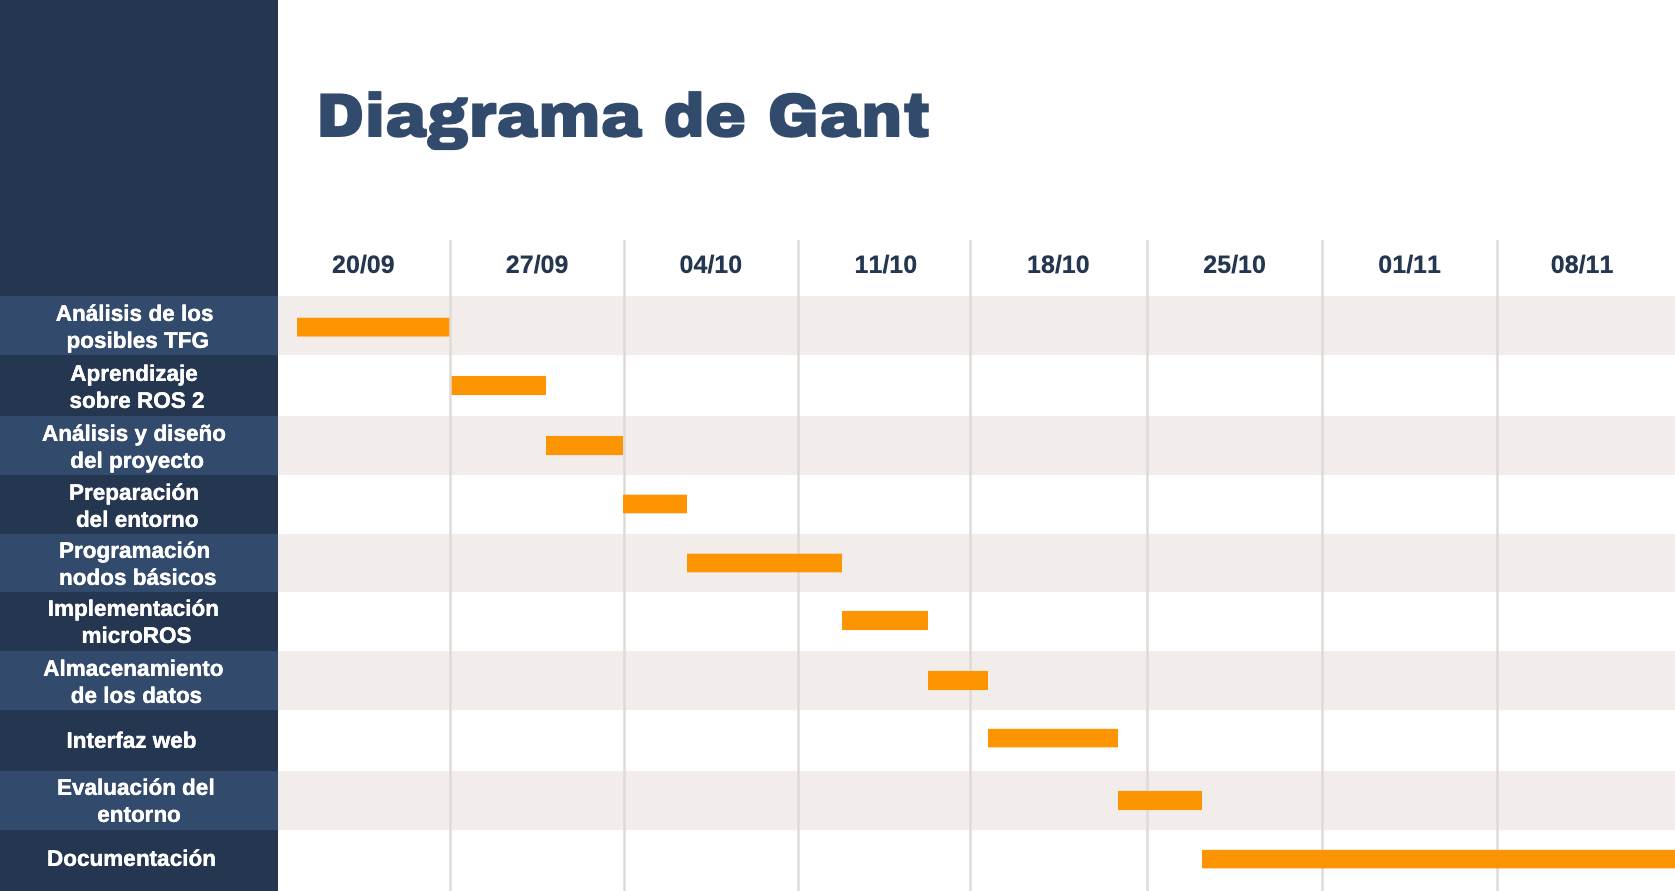
\includegraphics[width=\textwidth]{img/04-PreDiagrama-Gantt.png}
    \captionof{figure}{Diagrama de Gantt previo}
    \label{fig:pre-gantt}
\end{center}

Se van a explicar las diferentes categorías mostradas en el diagrama y que actividades abarcan cada una:

\begin{itemize}
    \item \textbf{Análisis de los posibles TFG.} Engloba la parte previa a la realización del proyecto, búsqueda de diferentes temáticas, información sobre las tecnologías a utilizar y casos de uso reales sobre este.
    \item \textbf{Aprendizaje sobre ROS 2.} Se agrupa el tiempo de aprendizaje de la tecnología y los conceptos relacionados.
    \item \textbf{Análisis y diseño del proyecto.} Una vez escogida la base del proyecto se establece la estructura del proyecto, elementos necesarios para su desarrollo tanto hardware y software, reestructuración de diferentes partes implementadas y derivados.
    \item \textbf{Preparación del entorno.} En los dispositivos utilizados es necesario la instalación y creación de un entorno de trabajo.
    \item \textbf{Programación nodos básicos.} Hace referencia a las implementaciones realizadas para los nodos principales a utilizar más el testeo de su funcionamiento.
    \item \textbf{Implementación microROS.} Para los microcontroladores utilizados, es necesario el uso de esta tecnología ya que no poseen un gran rendimiento para estas tareas.
    \item \textbf{Almacenamiento de los datos.} Toda la información generada en la red es almacenada en una base de datos.
    \item \textbf{Interfaz web.} Creación de una interfaz para mostrar los diferentes datos mencionados.
    \item \textbf{Evaluación del entorno.} Ejecución de diferentes nodos de manera progresiva con el hardware disponible.
    \item \textbf{Documentación.} Descripción de todo el trabajo realizado, recogido en este documento.
\end{itemize}

\section{Presupuesto}

En esta sección se van a tratar los costes de la realización de este proyecto, incluyendo tanto el hardware como el software, además de considerar las horas en su elaboración.

\begin{center}
    \centering
    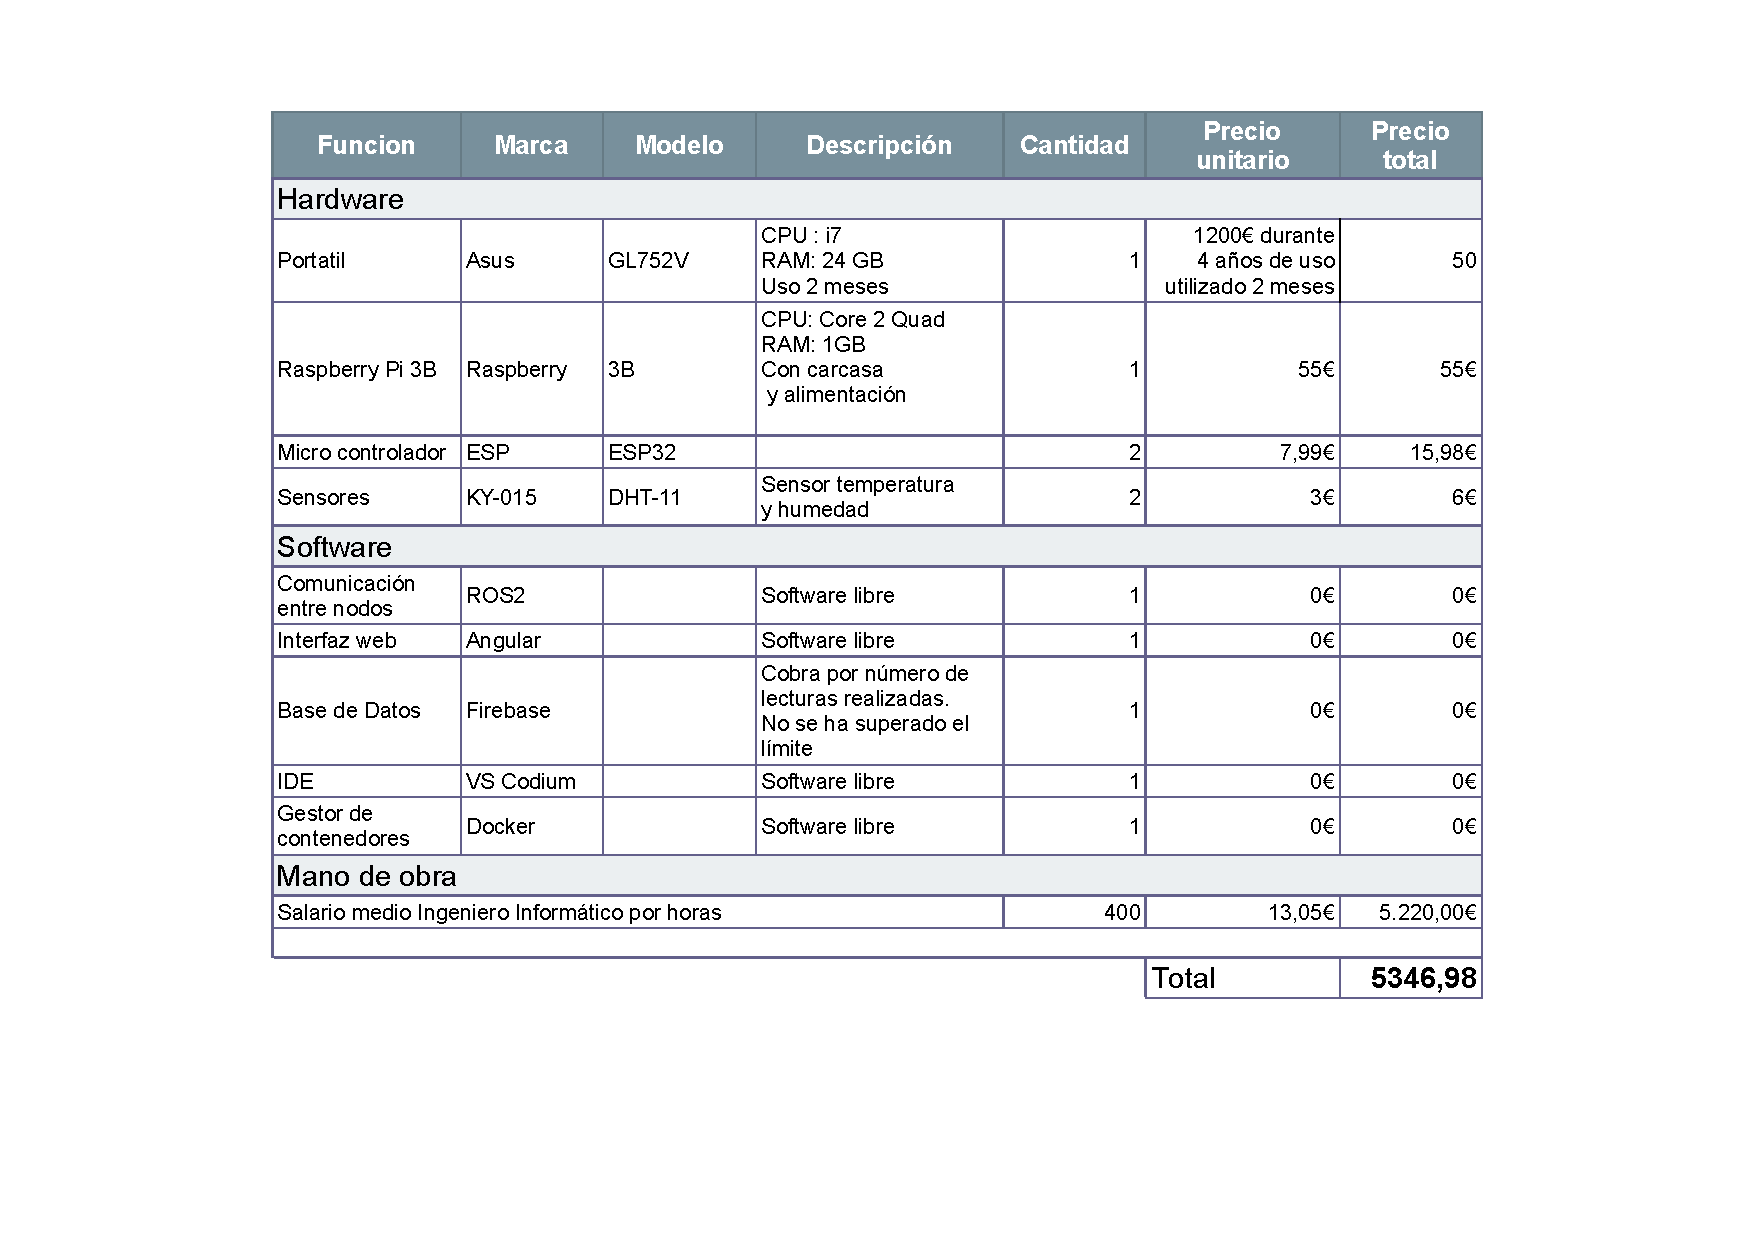
\includegraphics[width=\textwidth]{img/04-Presupuesto.pdf}
    \captionof{figure}{Presupuesto del proyecto}
    \label{fig:presupuesto}
\end{center}

El precio del portátil se ha hecho una estimación de la vida útil, con una media de 4 años, y como se ha utilizado durante 2 meses, el precio correspondiente es ese.

Por lo tanto, el gasto final será de 5346,98€ sumando las diferentes partes. A destacar del gráfico, el presupuesto de ingeniero informático ha sido obtenido de la web Talent.com \cite{salario}, con una media de 13,05€ la hora.

Hay que tener en cuenta que el escenario mayormente será virtual ya que respecto al hardware se van a utilizar diferentes elementos disponibles por casa. Si se tuviese que realizar un presupuesto real sería necesario contactar con diferentes personas con conocimientos relacionados a los sensores del mercado, cableado necesario, elementos para la comunicación, placas a utilizar y estancia de la web en un servidor.

En este caso respecto al hardware se va a utilizar un portátil para el desarrollo y despliegue, una Raspberry Pi 3B con Ubuntu Server y dos placas ESP32 con conectividad wifi junto a sensores DHT-11, cuyo coste se ve reflejado en la tabla anterior \ref{fig:presupuesto}.

\section{Tiempo total empleado}

En la figura \ref{fig:clockify} se pueden visualizar la distribución de horas final recogidas en la aplicación Clockify.

\begin{center}
    \centering
    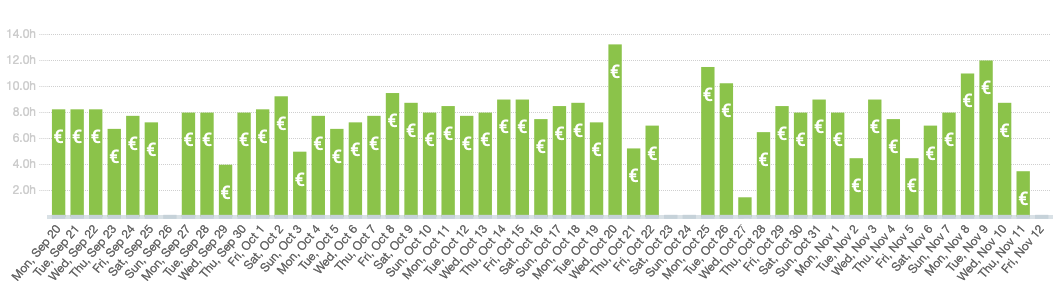
\includegraphics[width=\textwidth]{img/04-diagrama-horas.png}
    \captionof{figure}{Resumen de horas obtenido de Clockify juntando todas las diferentes tareas}
    \label{fig:clockify}
\end{center}

A fecha de la escritura de esta sección, el proyecto ha tomado unas 417h en realizarse, desde la búsqueda de que proyecto a realizar hasta la parte de documentación tras su finalización.

A continuación se adjunta el diagrama de Gantt tras apuntar las tareas realizadas:

\newpage

\begin{center}
    \centering
    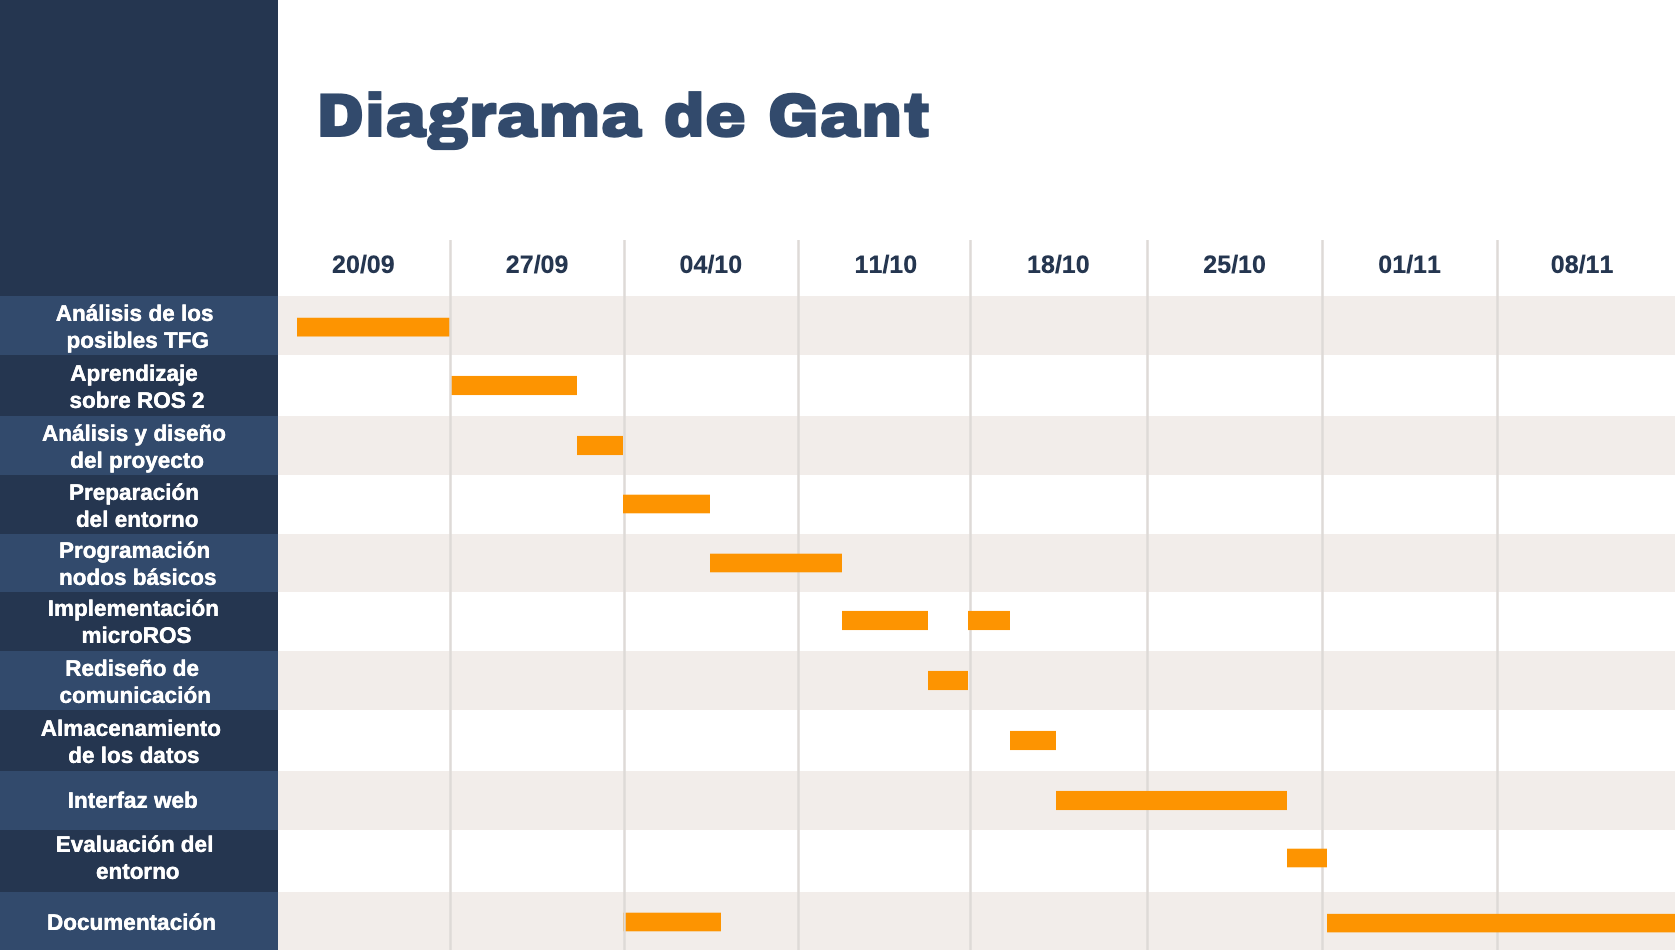
\includegraphics[width=\textwidth]{img/04-Diagrama-Gantt.png}
    \captionof{figure}{Diagrama de Gantt}
    \label{fig:gantt}
\end{center}

A destacar, la tarea del rediseño de comunicación que es la nueva. Esto fue debido a que el tipo de mensaje enviado necesitaba más información de la que se había añadido al principio.

	% Análisis del problema
	% 1. Análisis de requisitos
	% 2. Análisis de las soluciones
	% 3. Solucion propuesta
	% 4. Análisis de seguridad
	\chapter{Diseño de la propuesta}

En este capítulo se va a analizar los requisitos que tiene que tener este proyecto, que se va a abarcar en este trabajo, como va a ser la red de dispositivos que es necesario desplegar, de que tipo son e identificar que tarea va a realizar cada uno de estos nodos.

Para el análisis del escenario que se supone el contacto con un cliente propietario de un invernadero, obteniendo las medidas y el número de nodos necesarios. A partir de ahí se puede realizar un análisis de que es necesario para el despliegue del producto.

Con esta breve introducción, se van a identificar los requisitos que debe cumplir el proyecto. Tras esto se realizarán diferentes diseños para entender la estructura del código y de la red.

\section{Descripción del entorno y análisis de requisitos}

Para empezar, se va a suponer que tenemos un invernadero dividido en diferentes secciones. Estas se establecen en función del radio de actuación de algunos sensores o actuadores. Por lo tanto en cada una debe haber diferentes nodos que son necesarios para cumplir las expectativas y requisitos. Los dispositivos a desplegar se pueden agrupar en los siguientes apartados:

\subsection{Sensores}

En este proyecto y en la mayoría, los datos son la base de todo, sin ellos no se puede trabajar. Por ello se encuentran presentes diferentes generadores de estos datos, pudiendo ser como se ha comentado antes, sensores de temperatura, de humedad, de radiación, de la dirección del viento o velocidad, y algunos más.


Cada usuario necesita un tipo de estos productores según el cultivo que vaya a sembrar o la localidad del terreno. Además también hay que tener en cuenta el presupuesto, ya que según la calidad del sensor o el número de sensores que se requieran, hará que aumente el costo.


Dependiendo del tipo de cultivo, será necesario tener una mayor diversidad de dispositivos recopilando información. Hay más factores que influyen en este número, como el terreno en función de la cantidad de metros que disponga, la localización e incluso la inclinación de este. Se destacan estas últimas dos características ya que hay zonas donde el clima varía mucho entre el día y la noche.


Por tanto como se ha mencionado como requisito, es necesario poder aumentar el número de estos productores sin tener que tocar todo el sistema desplegado.

\subsection{Actuadores}

En el caso de tener productores, también es necesario dispositivos que consuman esos datos con un fin, en este caso realizar una acción, de ahí el nombre de actuadores.

Al igual que en el anterior caso, según las necesidades del usuario tendrá los actuadores divididos por secciones, o de forma más genérica. Un ejemplo práctico sería la calefacción, que podría tener una genérica para todo, o un sistema más individualizado

Además el cliente no tiene porqué automatizar todo, puede dejar trabajos manuales como las ventanas o controlar el riego.

\subsection{Controladores}

Estos dispositivos van a ser los nodos centrales por realizar una comparación con el esquema de las empresas. Deben que poder coexistir de manera conjunta varios de ellos en la red sin entorpecerse en sus tareas.

Tienen como objetivo recopilar toda la información del entorno, y en el caso de que se requiera, que puedan activar algunos de los actuadores que el usuario ordene. Por lo tanto tiene que ser capaz de sincronizar la interfaz con el estado de los dispositivos de la red.

Esta información recopilada tiene que ser almacenada, dando la opción que sea de manera local o en un servidor. Además deben poder gestionar todos esos datos y enviarlos si sea necesario.

\subsection{Interfaces de usuario}

Para que el usuario pueda acceder tanto a la información de monitorización como a la gestión de la plataforma, es necesario disponer de una interfaz de usuario.

Respecto a las interfaces a considerar, pueden encontrarse diferentes tipos de escenarios: situada en cada controlador donde una pantalla muestre los últimos datos, o  una interfaz web donde se puedan consultar los datos con unas credenciales, accesible a través de internet.

Dichas interfaces, a parte de mostrar los datos en forma de tablas, pueden tratarlos para mostrar gráficas, realizarse previsiones futuras o consultar el estado actual de los dispositivos.

Por último, sería necesario que a través de estas se pudiese controlar el estado de los diferentes actuadores. %, como hemos anteriormente.

\section{Requisitos de la plataforma a desplegar}

Tras haber planteado el entorno de trabajo y las diferentes categorías de dispositivos, se podrían agrupar los diferentes requisitos encontrados en el escenario:

\begin{itemize}
    \item El servicio tiene alta disponibilidad.
    \item Debe de existir una red IP donde se interconecten los dispositivos
    \item Los sensores deben tener uno o varios dispositivos de lectura del entorno.
    \item Los sensores deben publicar datos.
    \item Los actuadores deben tener uno o varios dispositivos para realizar diferentes acciones.
    \item Los actuadores deben poder leer los datos de los sensores.
    \item Los controladores deben leer todos los datos publicados por los nodos.
    \item Los controladores deben almacenar los datos.
    \item Deben de poder añadirse nuevos dispositivos a la red.
    \item Estos datos almacenados deben poder ser visualizados.
    \item Debe existir una conexión externa a internet para la subida de estos datos.
\end{itemize}

Tras este desglose de las funcionalidades que debe abarcar el proyecto, se puede proceder realizando el diseño de este para su posterior implementación.

\section{Diseño general del proyecto}

Por tener un ejemplo de un invernadero, podemos observar la imagen \ref{fig:invernadero_capilla}, de la web de Novagric \cite{novagric-invernadero}:

\begin{center}
    \centering
    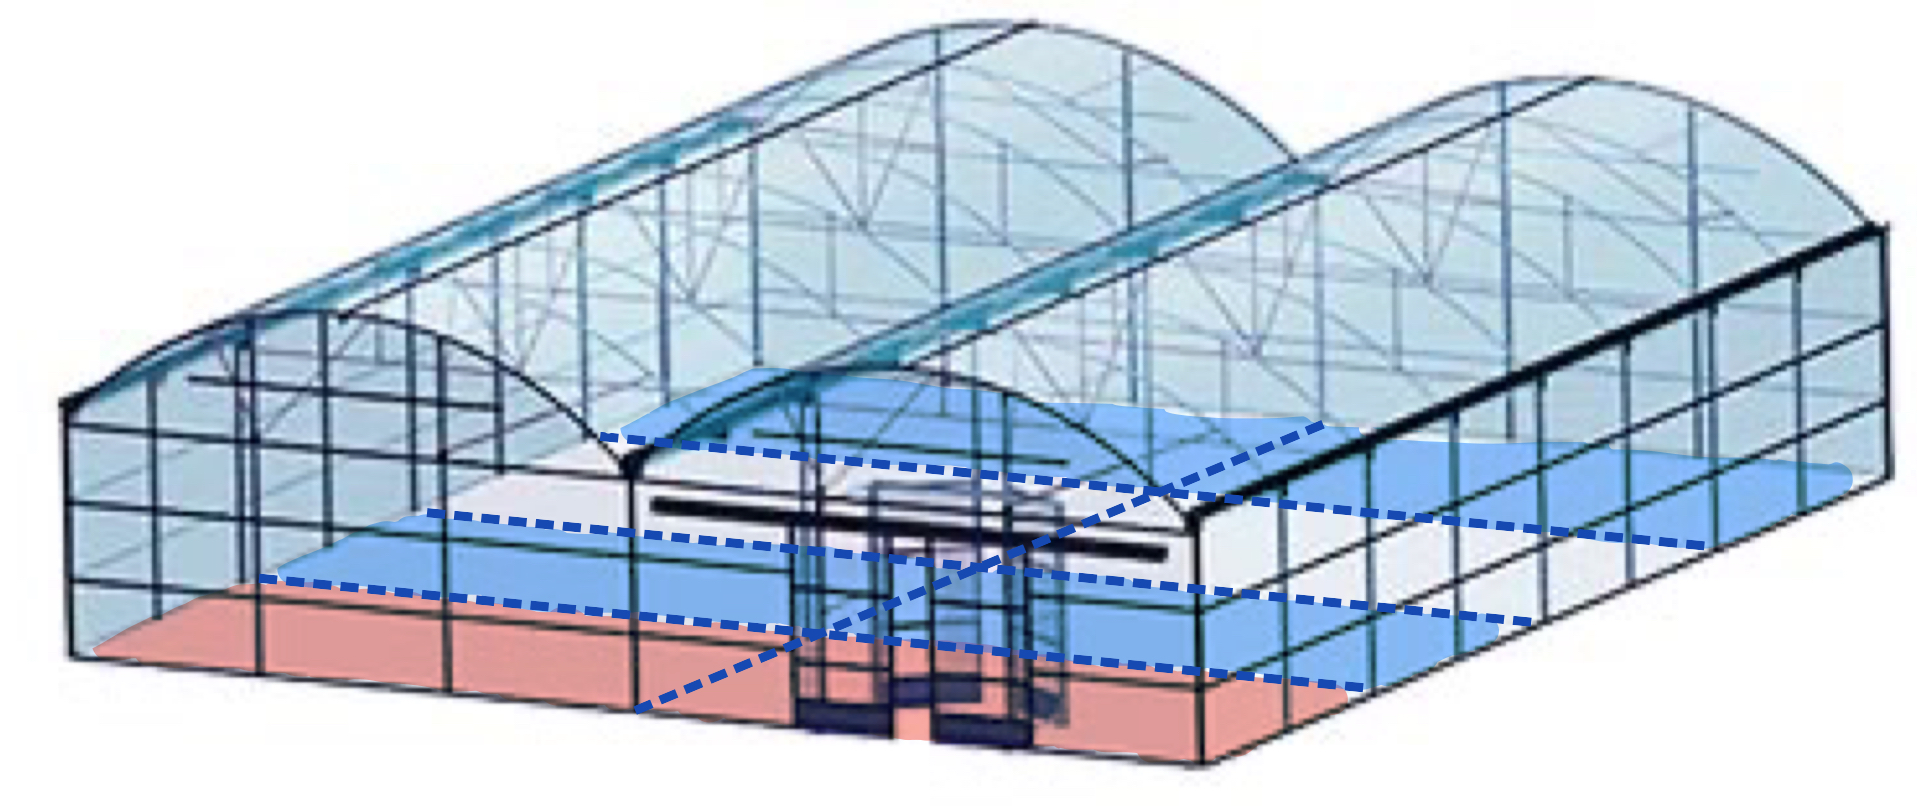
\includegraphics[width=\textwidth]{img/05-InvernaderoCapilla-Base.jpeg}
    \captionof{figure}{Dibujo de un invernadero tipo capilla (Novagric)}
    \label{fig:invernadero_capilla}
\end{center}

En base al dibujo anterior se va a plantear la división del terreno en 8 cuadrantes, mostrado con una vista aérea en el siguiente diagrama \ref{fig:invernadero_base}:

\begin{center}
    \centering
    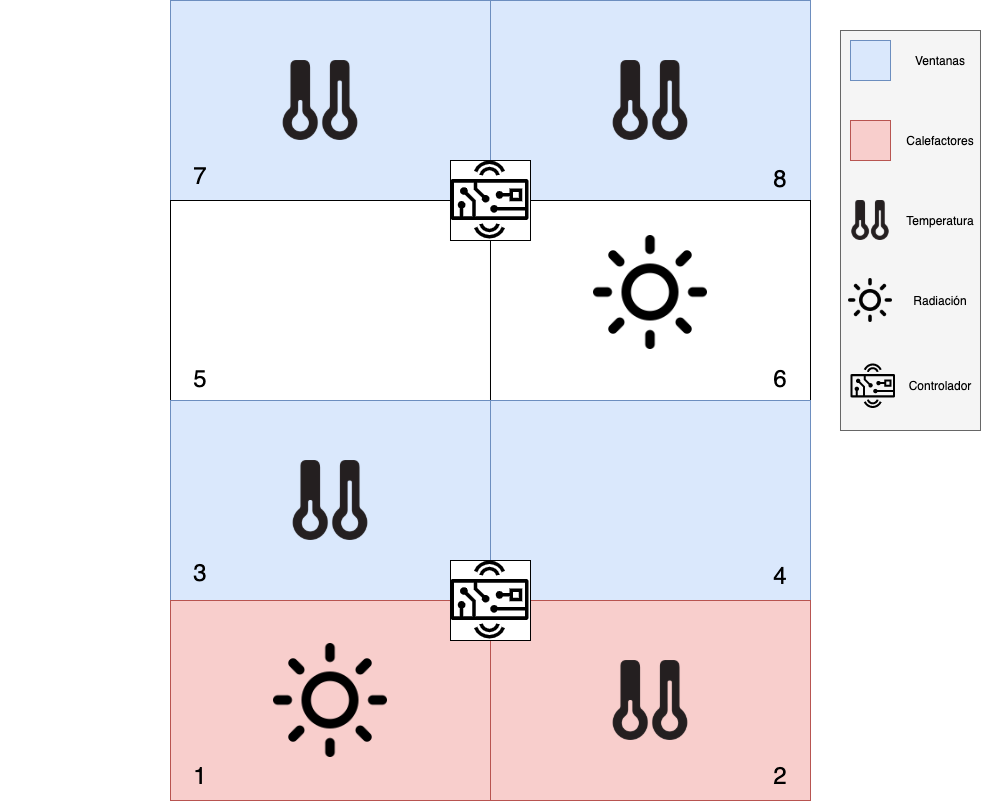
\includegraphics[width=\textwidth]{img/04-Invernadero_base.png}
    \captionof{figure}{Diagrama de un invernadero con vista aérea}
    \label{fig:invernadero_base}
\end{center}

Hay una leyenda en la figura indicando que es cada dispositivo, aclarando en la siguiente lista su funcionamiento:

\begin{itemize}
    \item \textbf{Sensor de temperatura.} Sensores situados en las zonas 2, 3, 7 y 8. Publica los datos recopilados.
    \item \textbf{Sensor de radiación.} Sensor situado en las zonas 1 y 6. Publica los datos recopilados.
    \item \textbf{Ventanas.} Cada recuadro azul indica que hay motores de ventanas en esa zona, como los mostrados en la figura \ref{fig:imagenes-actuadores}
    \item \textbf{Calefacción.} Cada recuadro rojizo hace referencia a la zona de actuación de los calefactores. En función de los datos suministrados por el sensor de temperatura 1 se activa o desactiva.
    \item \textbf{Controlador.} Encargado de recoger los distintos datos.
\end{itemize}

Además de estos dispositivos, hay un gestor de la base de datos para almacenar los datos recogidos por los controladores y una interfaz web. Estos no se han incluido en el escenario porque pueden estar desplegados en otro lugar.


\section{Diseño de clases de cada dispositivo}

Cada nodo mostrado como se ha podido ver durante el análisis dispone de diferentes conexiones y funciones a realizar, las cuales se van a ver reflejadas en la esta sección:

\begin{center}
    \centering
    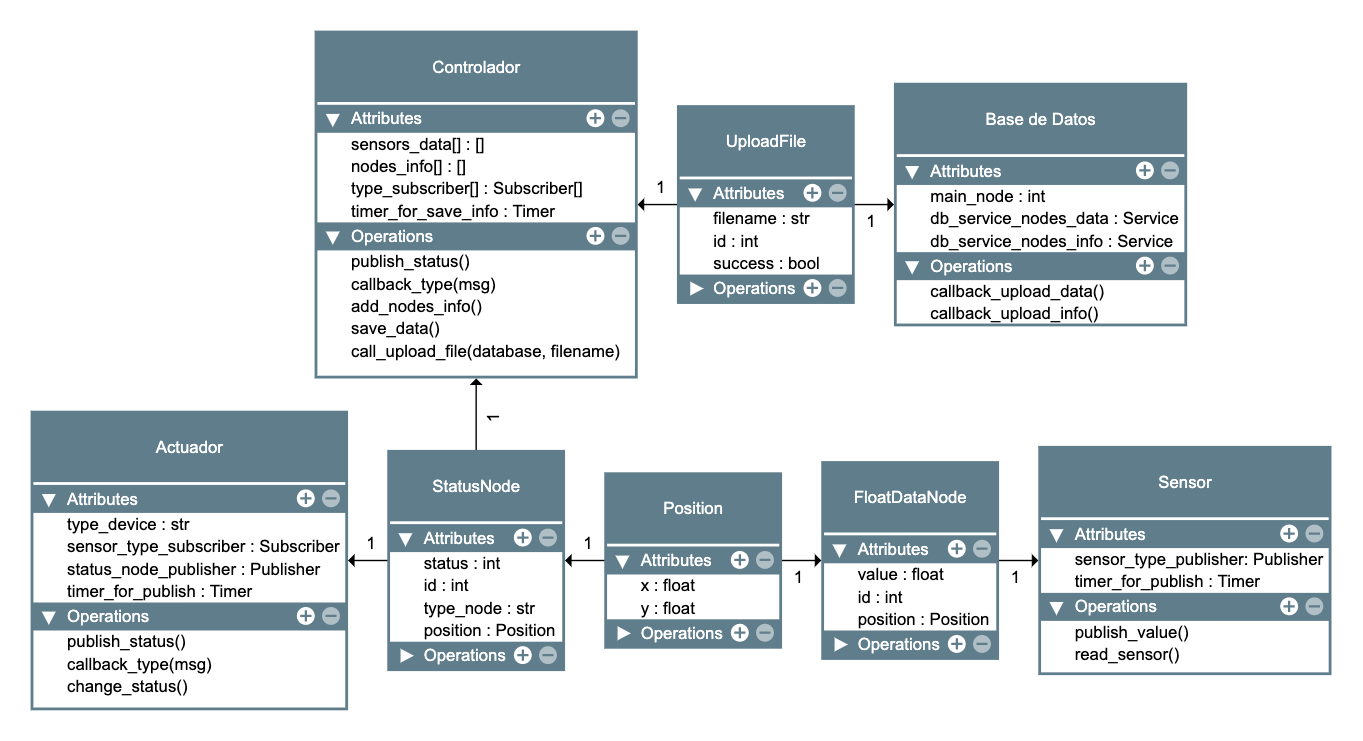
\includegraphics[width=\textwidth]{img/05-DiagramaClasesCompleto.png}
    \captionof{figure}{Diagrama de clases}
    \label{fig:diagrama-clases}
\end{center}

En este diagrama están representados los sensores y actuadores de manera genérica. En función del número de datos que recopile un sensor, existirá el mismo número de \textit{publicadores} o \textit{publishers}. Y en el caso de los datos necesarios por un actuador para realizar alguna acción, habrá ese mismo número de suscriptores.

Además en el caso del controlador, en el array mostrado \textit{type\_subscriber}, tendrá uno por cada tópico diferente en la red.

Las clases UploadFile, StatusNode, Position y FloatDataNode son autogeneradas a partir de un archivo por ROS2, por lo tanto están mostradas en la figura \ref{fig:estructuras-interfaces} de la siguiente sección.

\section{Diseño de interfaces en ROS2}

En esta sección se va a tratar la parte de comunicación entre los diferentes nodos. Para ello se tienen que definir las estructuras a utilizar para la comunicación, ya que es necesario indicar el tipo de mensaje a utilizar.

Un tópico \cite{topic} representa la unidad de información que puede ser producida o consumida por una aplicación DDS. ROS 2 las renombra interfaces debido a que las utiliza para comunicación publicador-suscriptor y cliente-servidor.

En el siguiente diseño se muestran las diferentes estructuras utilizadas.

\begin{center}
    \centering
    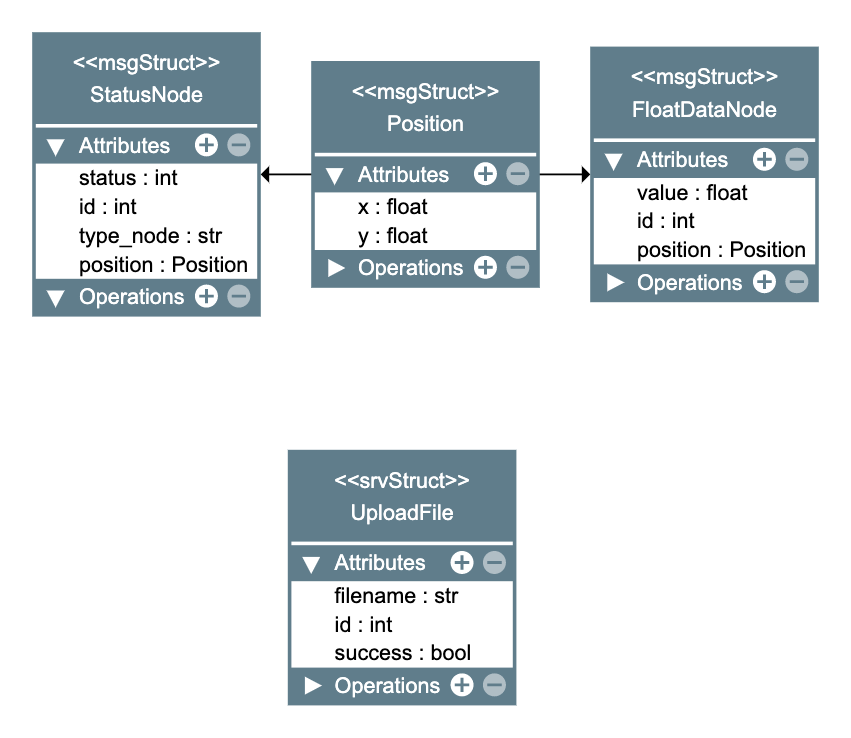
\includegraphics[width=\textwidth]{img/05-Interfaces.png}
    \captionof{figure}{Estructuras definidas utilizadas en los tópicos}
    \label{fig:estructuras-interfaces}
\end{center}

Estas estructuras en DDS se definen en archivos \ac{IDL}, los cuales definen una estructura estandarizada para todas las arquitecturas contempladas, y a partir de ella son generados los diferentes ficheros necesarios para utilizarlos como tipo de mensaje en un tópico. En ROS2 son conocidas como interfaces, subdivididas en dos grupos, los servicios y los mensajes. Estos pueden ser visualizados en las cabeceras de la figura anterior, explicadas a continuación:

\begin{itemize}
    \item \textbf{msgStruct}, hace referencia a un mensaje, utilizado de forma pub-sub en un tópico.
    \item \textbf{srvStruct}, hace referencia a un servicio, utilizado en una conexión cliente-servidor. Esta conexión se utiliza en la comunicación del Controlador y el gestor de la Base de Datos.
\end{itemize}

Ahora se van a analizar las diferentes interfaces utilizados en este despliegue, los cuales llevan asociado un tipo del conjunto anterior.

\begin{center}
    \centering
    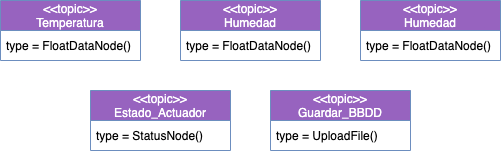
\includegraphics[width=\textwidth]{img/05-Topicos.png}
    \captionof{figure}{Interfaces}
    \label{fig:topicos}
\end{center}

Como podemos observar, existen 5 tipos de interfaces, 4 de ellas referentes a los nodos mostrados en el esquema \ref{fig:invernadero_base}, y otra referente al almacenamiento de los datos.

Cada uno de estos interfaces tienen asociadas un conjunto de \ac{QoS}, utilizados en ROS2 \cite{qos-ros}. QoS hace referencia a unas políticas de comunicación que se pueden establecer entre los nodos. En la siguiente lista se van a explicar las más destacables para este proyecto:

\begin{itemize}
    \item \textit{Keep last}, haciendo referencia al número de datos a almacenar en la cola, ya que si no se podrían almacenar todos.
    \item \textit{Queue size}, valor utilizado en \textit{keep last} si está asignado
    \item \textit{Reliable}, para asegurar que los datos lleguen a su destino
    \item \textit{Volatile}, no se hace intento de hacer persistentes las muestras.
\end{itemize}

Para finalizar esta sección, se va a mostrar un diagrama de comunicación entre los diferentes nodos, pudiendo observar como operan con los tópicos en la red.

Por aclarar, los diferentes nodos están mostrados con óvalos, y en el caso de los tópicos, se utilizan los rectángulos.

\begin{landscape}
\begin{figure}
    \centering
    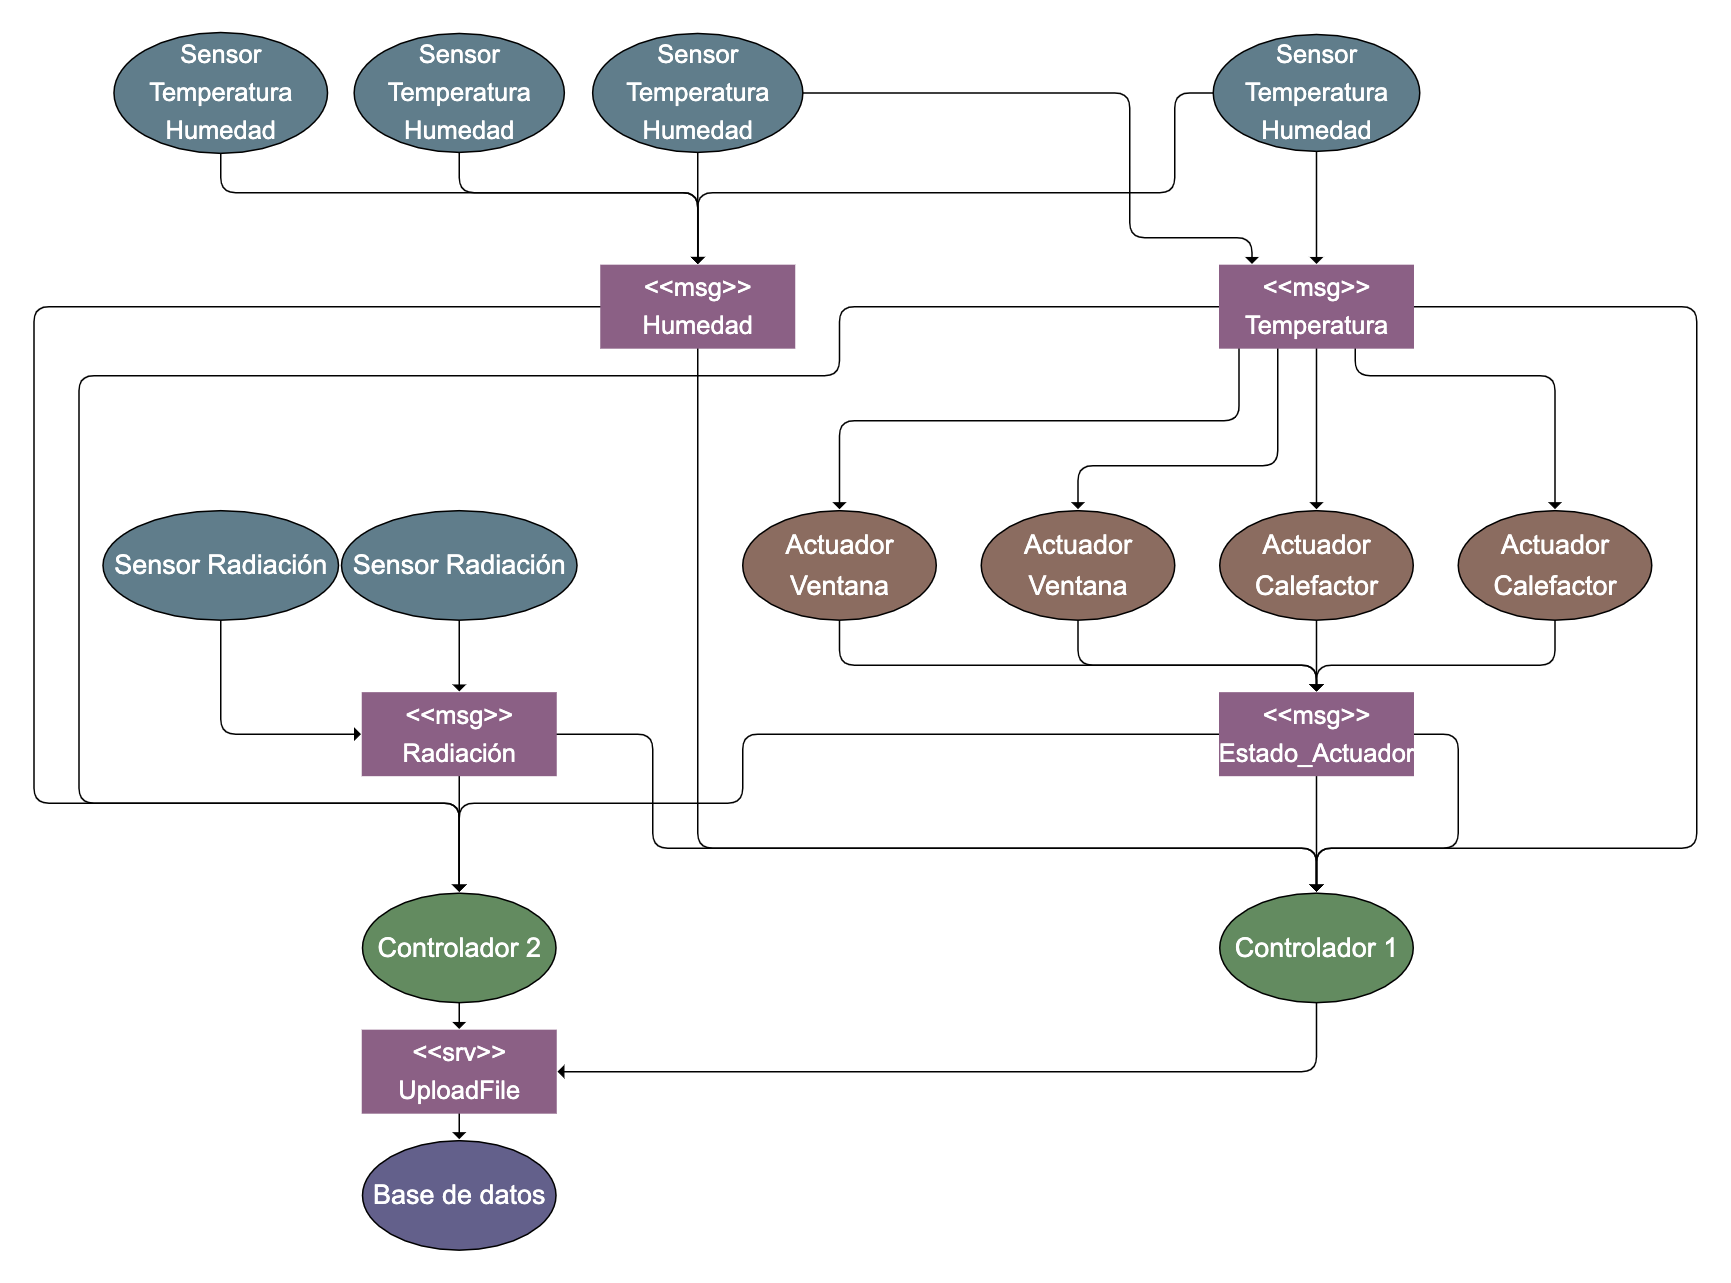
\includegraphics[width=1.6\textwidth]{img/05-DiagramaComunicacion.png}
    \caption{Diagrama de comunicación entre nodos}
    \label{fig:diagrama-comunicacion-nodos}
\end{figure}
\end{landscape}


\section{Diseño de la Base de Datos}

Tras las explicaciones de los datos tratados en las secciones anteriores, es necesario esquematizar que datos se van a guardar y como van a ser distribuidos. Para ello se van a definir dos tablas principales: sensores y actuadores. Estos deberán constar de los siguientes componentes:

\begin{itemize}
    \item \textbf{Id}. Almacena el id del dispositivo
    \item \textbf{Tipo}. Almacena el tipo de dato producido
    \item \textbf{Posición}. Almacena la posición del nodo
\end{itemize}

Aquí no se incluye ningún valor registrado sobre el estado del nodo o que valor esta obteniendo de los sensores, si no información más relacionada con su tipo o localización, información que varia poco a lo largo del tiempo. 

Únicamente va a existir una entrada por cada Id definido en la tabla. En el caso de que llegue nueva información por si el dispositivo se ha modificado su ubicación, o si transmite nuevos tipos de datos, esta entrada será actualizada.

Por otro lado, se va a tener una tabla por cada tipo de medida (temperatura, humedad...) y tipo de actuador (ventana, calefacción...). La estructura definida para este caso es:

\begin{itemize}
    \item \textbf{Id}. Id del dispositivo
    \item \textbf{Valor}. Valor recogido por el sensor, o estado del actuador
    \item \textbf{Timestamp}. Tiempo haciendo referencia a cuando se ha enviado este dato por la red.
\end{itemize}

Un ejemplo de tabla de \textit{Temperatura} con algunos datos seria la siguiente:

\begin{center}
\begin{tabular}{||c c c||} 
 \hline
 Id & Valor & Timestamp \\ [0.5ex] 
 \hline\hline
 11 & 23 & "10/26/21, 11:30:15" \\ 
 \hline
 12 & 21 & "10/26/21, 11:30:15" \\
 \hline
 13 & 20 & "10/26/21, 11:30:15" \\
 \hline
 11 & 22 & "10/26/21, 11:15:20" \\ 
 \hline
 12 & 21 & "10/26/21, 11:15:20" \\


 \hline
\end{tabular}
\captionof{figure}{Tabla de Temperatura}
\end{center}

En este caso se añade una entrada a la tabla por cada muestra obtenida, para luego poder visualizar los datos a lo largo del tiempo.


\section{Diseño de la interfaz web}

Esta es la parte final del capítulo, ya que tras analizar diseño a implementar, es necesario que el cliente pueda observar todos estos datos. Para ello se ha planteado un entorno web adaptable a distintos dispositivos desde donde se pueda interactuar para consultar información o mandar órdenes al sistema.

Este debe poder acceder a la base de datos mencionada anteriormente, y mostrar los datos en diferentes categorías.

La web debería constar de los siguientes componentes:

\begin{center}
    \centering
    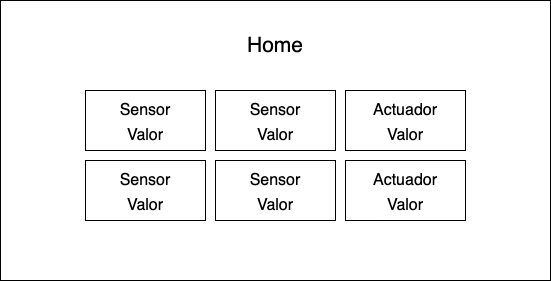
\includegraphics[width=\textwidth]{img/05-Web-home.png}
    \captionof{figure}{Página principal}
    \label{fig:home}
\end{center}

La página principal será la primera pantalla de la interfaz, donde se muestra en un dashboard el valor o estado actual de los diferentes nodos que hay desplegados en el escenario, pudiendo ver de un vistazo la información.

\begin{center}
    \centering
    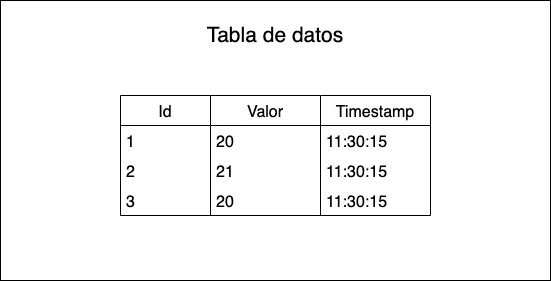
\includegraphics[width=\textwidth]{img/05-Web-tablas.png}
    \captionof{figure}{Tablas de datos}
    \label{fig:tablas-de-datos}
\end{center}

La figura anterior \ref{fig:tablas-de-datos} muestra todos los datos recopilados en la base de datos, subdivididas según el tipo de dato (temperatura, humedad..). Además sería conveniente poder buscar algún valor por hora, filtrar por id o incluso ordenar por parámetros.

\begin{center}
    \centering
    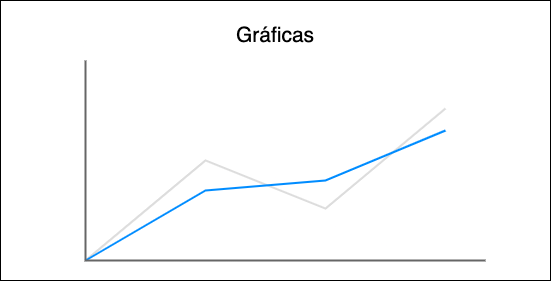
\includegraphics[width=\textwidth]{img/05-Web-charts.png}
    \captionof{figure}{Gráficas}
    \label{fig:graficas}
\end{center}

Sería idónea la implementación de una sección con los diferentes datos mostrados en gráficas, ya que facilita al usuario la interpretación y la visualización de la información respecto al tiempo, pudiendo comparar los diferentes sensores de una forma más sencilla.

 Además es complicado recordar que nodo esta situado en cada posición, por lo que un mapa con cada uno situado sería una funcionalidad a considerar. Esto vendría a ser similar a la figura \ref{fig:invernadero_base}. Para visualizarlo al igual que los ejemplos anteriores, se adjunta una imagen \ref{fig:mapa} a continuación del diseño planteado:
 
 \newpage
 
 \begin{center}
    \centering
    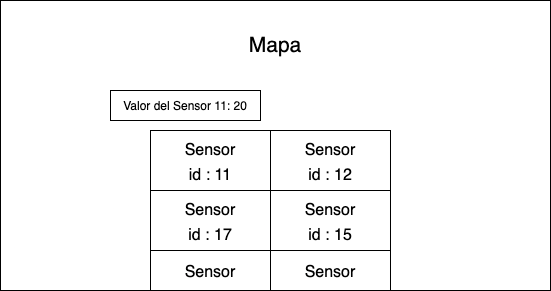
\includegraphics[width=\textwidth]{img/05-Web-map.png}
    \captionof{figure}{Mapa para visualizar la localización de los componentes}
    \label{fig:mapa}
\end{center}

Una funcionalidad interesante a implementar sería que seleccionar un sensor, el apartado de \textit{Valor del sensor} se actualice y muestre el estado actual de este.

	% Desarrollo bajo sprints: 
	% 	1. Permitir registros y login de usuarios
	% 	2. Desarrollo del sistema de incidencias
	% 	3. Desarrollo del sistema de denuncias administrativas y accidentes
	% 	4. Desarrollo del sistema de croquis
	%   5. Instalación de la aplicación de manera automática
	\chapter{Implementación}

El proceso de hacer realidad este proyecto y poder tenerlo desplegado ha tenido diferentes pautas a seguir, empezando por la parte de ROS 2, ya que era la esencial en el funcionamiento de nuestra plataforma.

Tras esto se han ido añadiendo las diferentes secciones comentadas en el análisis, haciendo una breve descripción de porqué se ha escogido esa tecnología para cada tarea, además de los diferentes problemas encontrados al realizarlo.

\section{ROS 2}

Para la creación del proyecto es necesario tener instalado ROS 2 y todas sus dependencias, explicado en la documentación de su web \cite{ros2}. En este caso se ha utilizado la versión Foxy.

Además hay que añadir diferentes scripts a nuestra shell para poder ejecutar los programas, o tener disponible el autocompletado de los comandos. Tras la instalación y configuración, se puede ejecutar algún programa de ejemplo para probar si se ha completado todo de manera correcta. 

ROS 2 trae diferentes herramientas, donde se van a destacar las más utilizadas en el proyecto:

\begin{itemize}
    \item \textbf{ros2 command}. Utilizado para diferentes tareas como ejecutar programas de ros2, creación de paquetes, consultar información de los nodos en ejecución, consulta de tópicos y más para cosas relacionadas con la parte de depuración.
    \item \textbf{colcon}. Utilizado para compilar el proyecto de ros, pudiendo seleccionar los diferentes paquetes por si está dividido en diferentes secciones.
    \item \textbf{rqt\_graph}. Herramienta gráfica que genera un esquema de la red con los diferentes nodos y tópicos, con sus respectivas conexiones, pudiendo mostrar u ocultar según unos parámetros a seleccionar.
\end{itemize}

Por lo tanto, para empezar se va a crear el entorno de trabajo, creando una carpeta para ello y tras esto, crear un directorio \textit{src} en su interior. Ahí tras ejecutar \verb|colcon build| que genera las diferentes carpetas necesarias se podrán crear los diferentes paquetes.

\subsection{Creación de las diferentes interfaces utilizadas en los tópicos}

Para poder utilizar los tópicos definidos en el análisis, es necesario crear un paquete donde se van a implementar esas interfaces. Para ello, situado en el directorio \verb|workdir/src| se ejecutaría el comando para crear un paquete, \verb|ros2 pkg create my_tfg_interfaces|.

Tras esto, será generada la carpeta \verb|my_tfg_interfaces|, donde se será necesario crear los diferentes directorios y ficheros, para tener una estructura similar a la siguiente:
\begin{lstlisting}[language=Bash, caption=Estructura del directorio de trabajo]
src/my_tfg_interfaces/
    msg/
        FloatDataNode.msg
        StatusNode.msg
        Position.msg
    srv/
        UploadFile.srv
    CMakeLists.txt
    package.xml
\end{lstlisting}

Tras esto, el código de los archivos creados \textit{.msg} y \textit{.srv} es muy simple, por lo que vamos a visualizar \verb|FloatDataNode.msg|:

\lstinputlisting[language=C, caption=Código FloatDataNode.msg]{code/FloatDataNode.msg}

Como se puede observar, solo hay que declarar las variables que se quieran utilizar en el envío. Esto es debido al uso de IDL, que solo hace necesario la definición de estas, ya que ROS genera los diferentes ficheros necesarios. Por aclarar,  \verb|Position| en este caso es otro archivo, como si fuese un objeto con las otras variables.

En el caso de los servicios, el formato cambia un poco ya que hay un \textit{request} y un \textit{reply}, por lo tanto se escribe dividido como en el ejemplo a continuación:

\lstinputlisting[language=C, caption=Código UploadFile.srv]{code/UploadFile.srv}

Este código corresponde a \verb|UploadFile.srv|, utilizado en la comunicación del nodo controlador y el nodo gestor de la base de datos.

Tras esto sería necesario modificar los archivos \textbf{CMakeList.txt} y \textbf{package.xml}, añadiendo las dependencias correspondientes y los archivos creados.

Por último, tras cada nuevo elemento o modificación de cada paquete, es necesario volver a compilar cada paquete. 

\subsection{Desarrollo de los nodos}

Al igual que se ha creado un paquete en el punto anterior, en este caso se aplicaría el mismo procedimiento, pero el comando no sería exactamente el mismo, ya que sería necesario indicar el tipo de lenguaje a utilizar.

Como lenguaje se va a utilizar Python, aunque sería posible utilizar otros lenguajes, como C++. Por lo tanto para generar el paquete ejecutamos:

\begin{lstlisting}[language=Bash, caption=Comando para la creación de un paquete de Python con ROS 2]
ros2 pkg create my_tfg_pkg --build-type ament_python \
--dependencies rclpy
\end{lstlisting}

Esto es para la creación del paquete especificando el tipo de lenguaje y las dependencias, en este caso \textit{rclpy} que contiene todo lo necesario para poder desarrollar los nodos.

Tras todo esto, el directorio tendría la siguiente estructura:

\begin{lstlisting}[language=Bash, caption=Estructura del directorio de desarrollo con Python]
src/my_tfg_pkg/
    my_tfg_pkg/
        __init__.py
    test/
    resource/
    setup.cfg
    setup.py
    package.xml
\end{lstlisting}

Para poder construir los diferentes nodos, tenemos que añadir los respectivos ficheros en la carpeta \verb|src/my_tfg_pkg/my_tfg_pkg|.

Antes de empezar con la implementación, según la comunidad, la estructura estándar de los nodos tiene que ser la siguiente:

\newpage

\lstinputlisting[language=Python, caption=Plantilla genérica para la creación de nodos]{code/template-node.py}


Se puede observar en el código un método \textit{main} donde se crea un objeto de nuestra clase, y con el método \textit{spin}, se mantiene en ejecución ese nodo. Con esta base ya se pueden empezar a crear los nodos necesarios.

Por tanto, se va a repasar los diferentes nodos de manera genérica:

\begin{itemize}
    \item \textbf{Sensores.} Productores de información.
    \item \textbf{Actuadores.} Consumidores de esos datos, y productores de otros.
    \item \textbf{Controladores.} Encargados de recopilar todos los datos.
\end{itemize}

En las figuras mostradas durante el análisis, podemos observar el diseño definido de estos archivos concretamente en la \ref{fig:diagrama-clases}.

\subsubsection{Sensores}

Van a realizar una lectura del sensor cada cierto tiempo, llamando al método \verb|read_sensor()|. Esta función será la principal diferencia entre este tipo de nodo, ya que para su implementación será necesario una librería u otra. Tras esta lectura, estos datos serán publicados en la red. Para ello es necesario tener:

\begin{itemize}
    \item Un \textbf{publisher}, que defina el tópico donde se va a publicar
    \item Un \textbf{timer}, que establezca el tiempo cada vez que se va a realizar esa publicación. Este tendrá como parámetro la función de \verb|publish_value()|, que será llamada en el periodo definido.
\end{itemize}

Su declaración viene explicada en la documentación \cite{ros2}, pero por abreviar la búsqueda, esta se realiza de la siguiente forma:

\begin{lstlisting}[language=Python, caption=Publisher del sensor de temperatura]
self.temperature_publisher_ = 
    self.create_publisher(FloatDataNode, "temperature", 10)
self.sensor_timer_ = 
    self.create_timer(20.0, self.publish_temperature_data)
\end{lstlisting}

Se va a definir el \verb|publisher|, ya que los argumentos pueden ser confusos:

\begin{itemize}
    \item \textbf{FloatDataNode}, hace referencia al tipo de dato publicado en el tópico
    \item \textbf{"temperature"}, es el nombre del tópico donde se van a publicar los datos
    \item \textbf{10}, hace referencia al número de mensajes a conservar en el historial. También se puede declarar un elemento QoSProfile donde declaremos las diferentes QoS \cite{qos-ros} a aplicar.
\end{itemize}

El \verb|timer| recibe como parámetros el tiempo y la función que va a llamar, donde el \verb|publisher| publica el mensaje.

Según el los diferentes tipos de sensores que tenga conectados este nodo, le será necesario ese mismo número de \verb|publishers| con sus respectivas funciones.

\subsubsection{Actuadores}

A diferencia de los sensores, estos van a tener un \verb|publisher| para el estado de este nodo, el \verb|timer| para la publicación de esta información y un \verb|subscriber|.

Este \verb|subscriber| es el nuevo añadido a diferencia del anterior nodo. Para ver su estructura vamos a visualizar la siguiente declaración:

\begin{lstlisting}[language=Python, caption=Subscriber del actuador]
self.temperature_subscriber_ = self.create_subscription(
  FloatDataNode, "temperature", self.callback_sensor_data, 10)
\end{lstlisting}

Los parámetros hacen referencia al tópico del que se quieren leer los datos. El método \verb|callback_sensor_data| maneja los datos recibidos, comparando la temperatura en este caso con un posible valor de acción. Como se comenta en la parte de análisis, un ejemplo es cuando la temperatura baje de 12ºC, la calefacción se encienda y tras esto, se publique el nuevo estado.

\subsubsection{Controladores}

El nodo \textbf{controlador} posee más funcionalidades que los anteriores, ya que está orientado a utilizarse en un dispositivo central con más potencia.

Posee un \verb|subscriber| por cada tipo de tópico en la red, y tras la recepción de cada dato es guardado en un diccionario de Python. Este diccionario tras un tiempo definido con un timer almacena los datos en un json, para posteriormente contactar con el nodo gestor de la base de datos. Esto lo hace en los dos métodos siguientes

\begin{lstlisting}[language=Python, caption=Creación de cliente de ROS2 en Python]
def call_upload_file(self, json_name):
    client = self.create_client(UploadFile, "upload_db")
    while not client.wait_for_service(1.0):
        self.get_logger().warn("Waiting for DB Service...")

    request = UploadFile.Request()
    request.device_id = self.status_controller_.device_id
    request.filename = json_name

    future = client.call_async(request)
    future.add_done_callback(
        partial(self.callback_upload_file,
                device_id=self.status_controller_.device_id,
                filename=json_name))

def callback_upload_file(self, future, device_id, filename):
    try:
        response = future.result()
        if response.success:
            self.get_logger().info("Upload to Database done.")
    except Exception as e:
        self.get_logger().error("Service failed %r" % (e,))
\end{lstlisting}

Aquí se está gestionando una comunicación cliente-servidor, debido a que pub-sub no es la más indicada en este caso, ya que es necesario la obtención de respuesta por parte del gestor de la base de datos.

Se pueden visualizar métodos asíncronos ya que no se puede detener la ejecución del controlador de almacenar los demás datos que llegan en ese tiempo.

Por estructurar el código mostrado, primeramente se crea el cliente según el tópico a utilizar y se espera una conexión por parte del servidor. Tras esto se crea el objeto request que va a ser enviado. Por último se realiza la espera asíncrona de la response, y según su valor, se muestra en el gestor de logs que ha sido subido o se lanza una excepción.

\subsubsection{Ejecución y herramientas utilizadas}

Terminando esta sección se van a mostrar en las siguientes capturas la ejecución de los nodos, diferentes herramientas en la shell con el comando ros2, y por último el estado de la red mostrado con rqt\_graph.

\newpage

 \begin{center}
    \centering
    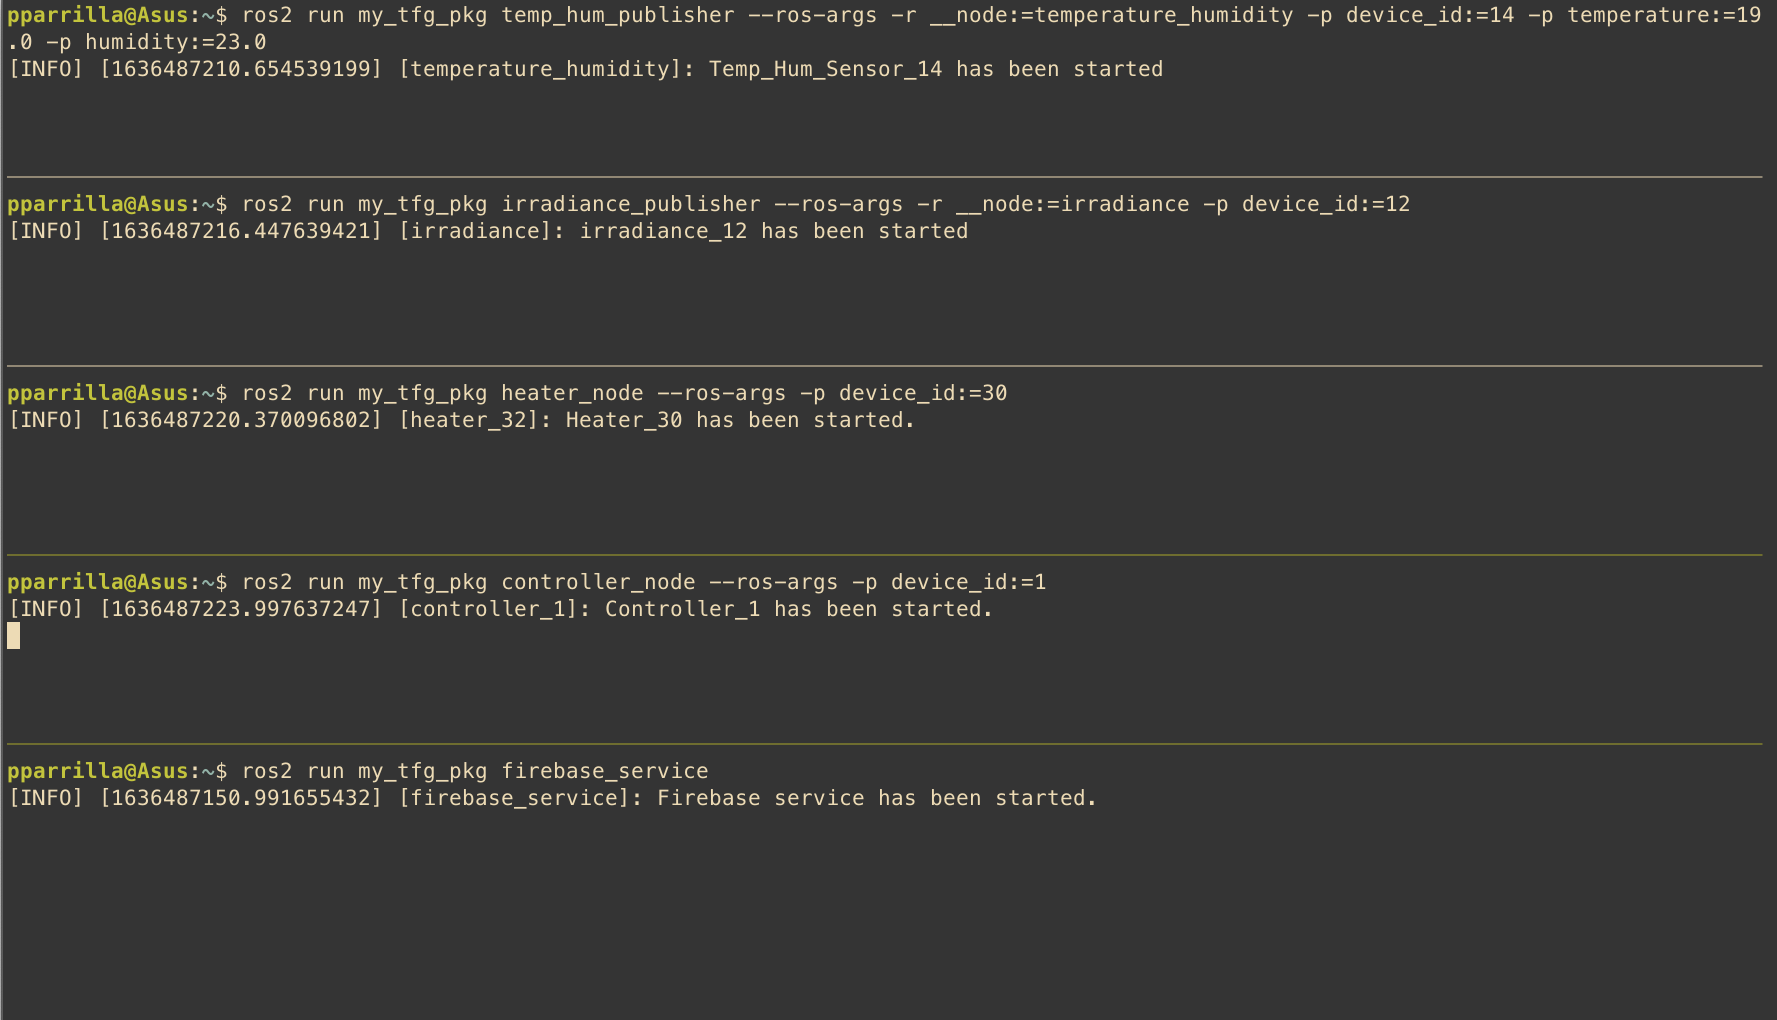
\includegraphics[width=\textwidth]{img/06-Ejecucion-nodos.png}
    \captionof{figure}{Ejecución de los diferentes nodos con parámetros}
    \label{fig:ejecucion-nodos}
\end{center}

Estos parámetros hacen referencia al id del dispositivo o al valor de temperatura que va a estar emitiendo ese nodo, ya que actualmente son virtuales y no leen de ningún sensor físico.

 \begin{center}
    \centering
    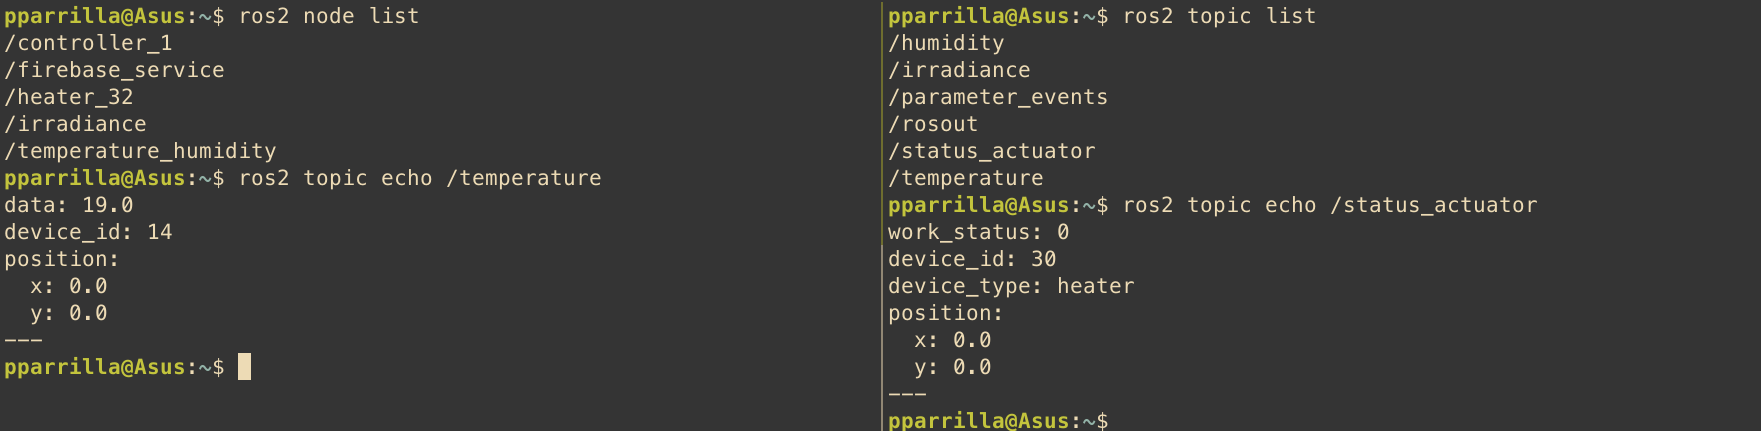
\includegraphics[width=\textwidth]{img/06-Tools.png}
    \captionof{figure}{Herramientas con el comando ros2}
    \label{fig:tools-ros2}
\end{center}

Se pueden observar distintos comandos de ros2 en la anterior figura:

\begin{itemize}
    \item \textbf{ros2 node list} muestra la lista de nodos actualmente ejecutandose en la red
    \item \textbf{ros2 topic list} muestra la lista de tópicos en la red
    \item \textbf{ros2 topic echo /temperature} muestra por pantalla los datos publicados referentes a ese tópico de temperatura
\end{itemize}

Hay más comandos similares, como \verb|ros2 interfaces show interface.msg| que mostraría las variables que implementa esa interfaz, muy útil cuando se utilizan interfaces no propias. Pero los más utilizados son los mostrados en la figura \ref{fig:tools-ros2}.

 \begin{center}
    \centering
    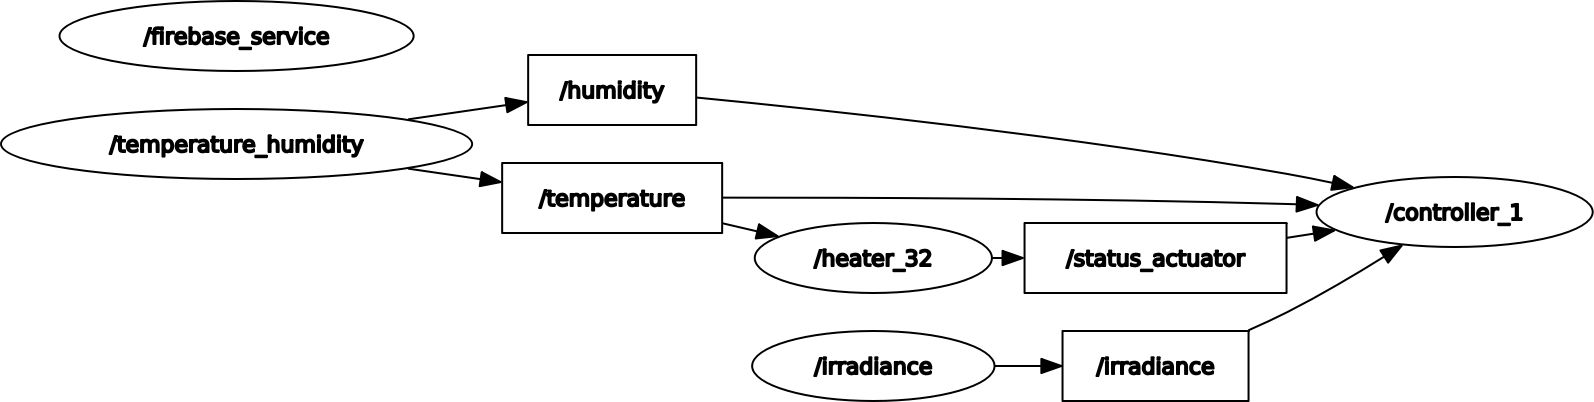
\includegraphics[width=\textwidth, height=4.5cm]{img/06-Rosgraph.png}
    \captionof{figure}{Gráfico generado con rqt-graph de la red}
    \label{fig:rqt-graphs}
\end{center}

Por aclarar al igual que en la figura \ref{fig:diagrama-comunicacion-nodos} los nodos están representados con el óvalo, y los rectángulos son los tópicos.

Esta herramienta, como se ha comentado, genera un gráfico de los distintos nodos y tópicos ejecutandose en la red, mostrando la comunicación existente. Los tópicos utilizados en conexiones cliente-servidor no los añade a la red, por eso \verb|controller_1| y \verb|firebase_service| no aparecen conectados.


\subsection{Micro ROS en microcontroladores}

Además de la utilización de ROS 2 en este proyecto, se han querido utilizar microcontroladores ya que son utilizados en casi cualquier producto robótico, estas tienen una baja latencia en cuestión a trabajo a tiempo real y consumen menos energía, además de su precio que suele ser más económico.

Para ello, es necesario la utilización de micro-ROS \cite{micro-ros}, que es la adaptación de la tecnología a estos microcontroladores. Además ha sido necesario utilizar FreeRTOS \cite{free-rtos}. Esto es un sistema operativo a tiempo real donde encima se va a ejecutar micro-ROS.

Una vez preparado el entorno como viene explicado en la documentación de micro-ROS, es necesario crear los siguientes ficheros:

\begin{itemize}
    \item \textbf{app.c}, que contiene la aplicación que se va a ejecutar
    \item \textbf{app-colcon.meta}, que contiene la información especifica necesaria para la compilación con \textit{colcon}.
\end{itemize}

Como se puede observar, ahora hay que utilizar C como lenguaje, donde no existen las clases, por tanto la estructura del fichero va a variar, pero no mucho ya que se realizará la mayoría de cosas en el propio main, llamando a diferentes métodos.

El objetivo va a ser utilizando una placa ESP32 leer de un sensor DHT-11 la temperatura y humedad, por lo tanto es necesario también incluir en el proyecto la librería especifica para realizar la lectura de datos.

La creación de un publisher y un timer en este caso ha sido la siguiente:

\begin{lstlisting}[language=C, caption=Publisher Timer y Executor en C para microcontrolador]
// create publisher for temperature
RCCHECK(rclc_publisher_init_default(
        &temperature_publisher,
        &node,
        ROSIDL_GET_MSG_TYPE_SUPPORT(custom_node_message, msg, 
                                        FloatDataNode),
        "temperature"));
        
// create timer
rcl_timer_t timer;
const unsigned int timer_timeout = 30000;
RCCHECK(rclc_timer_init_default(
        &timer,
        &support,
        RCL_MS_TO_NS(timer_timeout),
        timer_callback));

// create executor
rclc_executor_t executor;
RCCHECK(rclc_executor_init(&executor, 
                        &support.context, 1, &allocator));
RCCHECK(rclc_executor_add_timer(&executor, &timer));
\end{lstlisting}

Tras esto, cada 30 segundos se ejecuta la función \verb|timer_callback| que se encarga de leer los datos del sensor y publicarlos.

Ya con la aplicación operativa y todas las dependencias añadidas, sería momento de construir el proyecto y flashearlo en el microcontrolador.

El montaje del sensor y la placa tendría la siguiente estructura:

\newpage

 \begin{center}
    \centering
    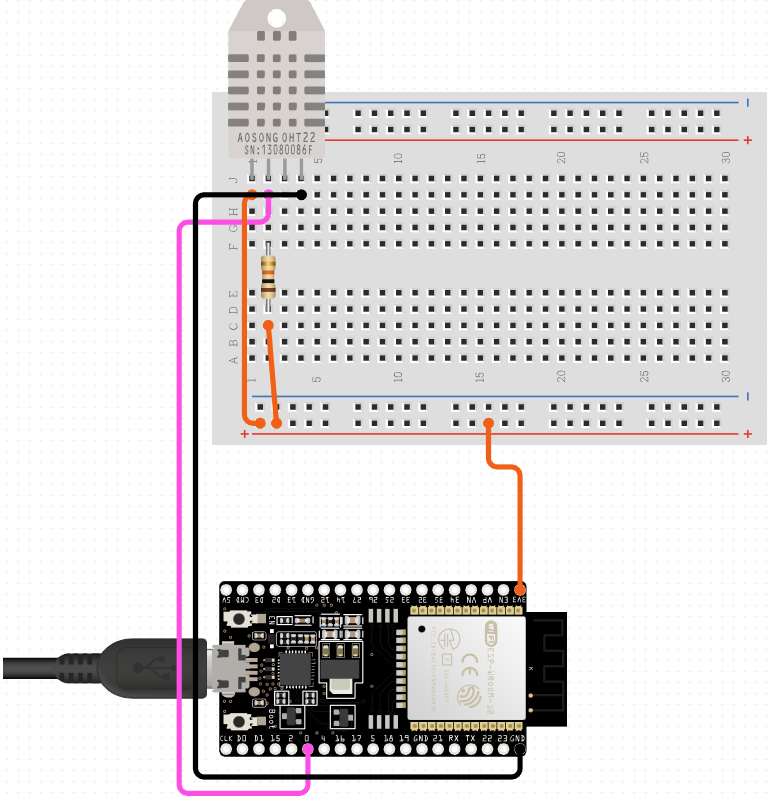
\includegraphics[width=0.6\textwidth]{img/06-DiagramaESP32.png}
    \captionof{figure}{Montaje ESP32 con DHT11}
    \label{fig:esp32-dht11}
\end{center}

Hay que tener en cuenta, que micro-ROS necesita la existencia de un agente para que el microcontrolador pueda contactar con el resto del proyecto de ROS 2. Este puede ser ejecutado en un contenedor de Docker \cite{docker} con el siguiente comando:

\begin{lstlisting}[language=Bash, caption=Ejecución Agente de micro-ROS en un contenedor Docker]
docker run -it --rm --net=host microros/micro-ros-agent:foxy \ 
    udp4 --port 8888 -v6
\end{lstlisting}

Este contenedor debería estar ejecutando en uno de los controladores distribuidos por el escenario, o en otro dispositivo dedicado para ello.

\subsection{Conexión a la base de datos}

Como se ha comentado, cada controlador almacena la información en un fichero tipo .json, y tras esto contacta con el gestor de la base de datos mediante cliente-servidor. Para ello tiene que enviar su id y el nombre el fichero.

Por lo tanto, el nodo de conexión a la base de datos debe tener las librerias para poder conectarse a esta.

En este caso se han implementado 2 nodos diferentes:

\begin{itemize}
    \item \textbf{Nodo Firebase.} Este realiza una conexión con Firebase \cite{firebase}, donde el archivo será estructurado en colecciones y documentos según define esta tecnología. El motivo a utilizar esta base de datos es el alojamiento en la nube, ya que facilita el acceso a los datos mediante las distintas plataformas. La librería para poder realizar la conexión es \textit{firebase\_admin}.
    \item \textbf{Nodo SQLite3.} Este crea una conexión con SQLite3 \cite{sqlite3} donde se almacenarán los datos de manera local del dispositivo en formato de tablas. Este puede estar ejecutado en cada dispositivo donde se ejecuta el nodo controlador, pudiendo tener la información replicada. La librería para poder realizar la conexión es \textit{sqlite3}.
\end{itemize}

En cada nodo es necesario presentar una estructura de creación del servidor, método para gestionar la llamada y otro método para subir la información a las respectivas bases de datos. 
% Todo este código puede ser visualizado haciendo click \href{https://github.com/pparrilla/ROS2_TFG/blob/main/src/my_tfg_pkg/my_tfg_pkg/firebase_service.py}{aquí}.

La explicación para el uso de dos bases de datos distintas...


\subsection{Simulación de un entorno con diferentes nodos}

Tras haber implementado los diferentes nodos, en caso de realizar una simulación del escenario descrito, no es viable la opción de ejecutar cada nodo de manera individual en una terminal como se muestra en la figura \ref{fig:ejecucion-nodos}, ya que en este caso se quieren lanzar unos 15-20 nodos aproximadamente.

Para estas ocasiones, ROS 2 dota de un tipo de archivo llamado \textit{Launch File}. En este se pueden incluir los diferentes nodos que se quieren ejecutar, indicando los parámetros como el nombre, el valor a producir, la posición y los demás que se hayan asignado durante el desarrollo de estos.

Por lo tanto da la posibilidad de generar un escenario y ejecutarlo desde un fichero, con el comando \textit{ros2 launch}.

Para su uso sería necesario la creación de otro paquete al igual que en los anteriores casos, y tras esos en un archivo tipo \textit{name.launch.py} escribir el código necesario, importanto la libreria \textit{launch}.

Tras el desarrollo y la ejecución de este fichero, con \textit{rqt\_graph} podemos observar la red de la siguiente forma:

\newpage

 \begin{center}
    \centering
    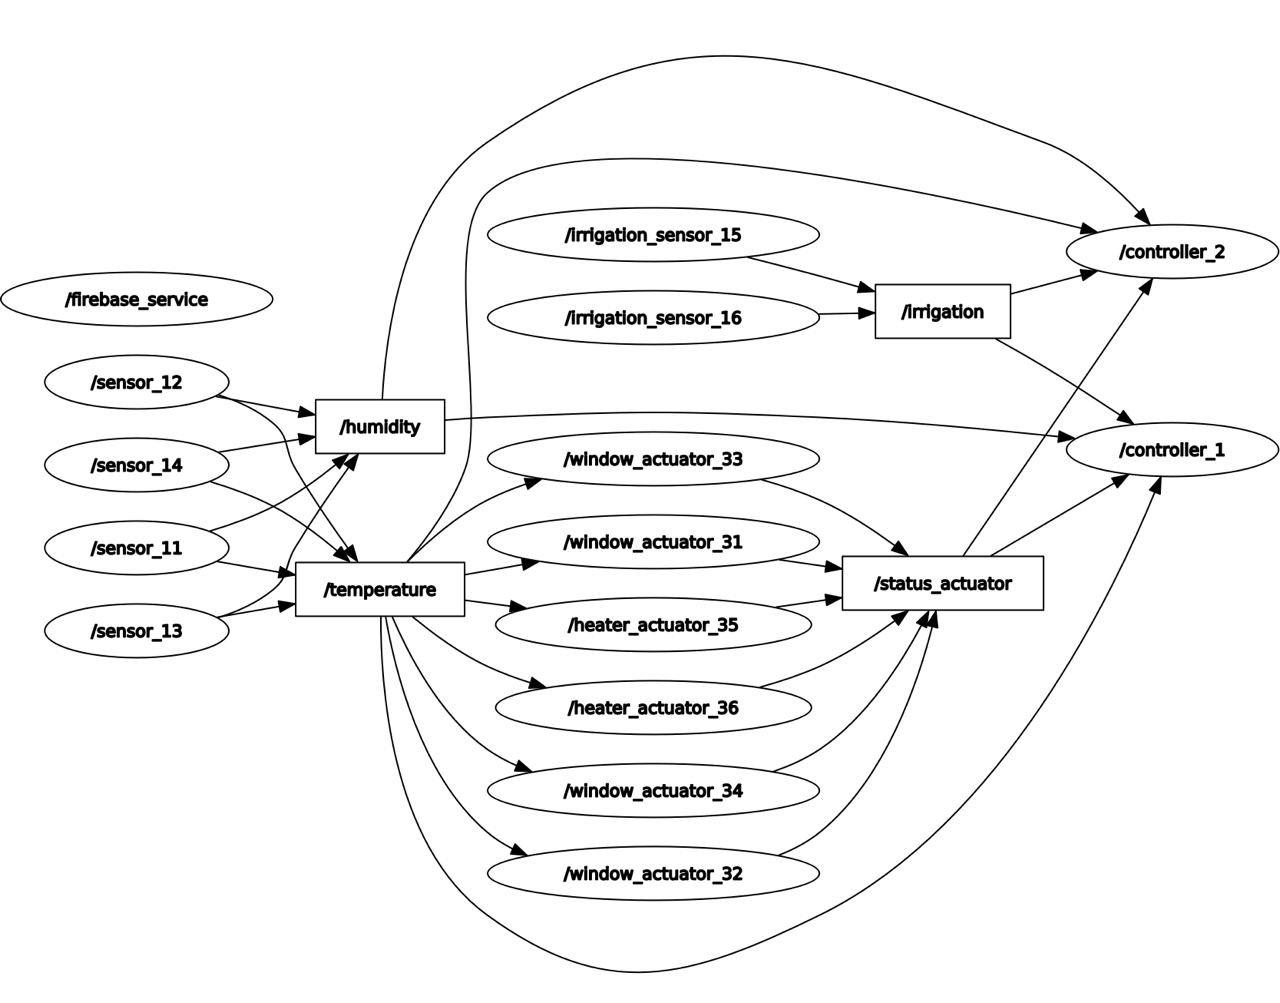
\includegraphics[width=\textwidth]{img/06-Rqt-graph.jpeg}
    \captionof{figure}{Simulación del escenario en la red}
    \label{fig:simulacion-escenario-nodos}
\end{center}

Al igual que en el anterior caso \ref{fig:rqt-graphs}, los óvalos son los nodos y los rectángulos los tópicos.

Este escenario ha sido desplegado utilizando los siguientes dispositivos:

\begin{itemize}
    \item \textbf{2 placas ESP32}, siendo los sensores 11 y 12, leyendo la información de los sensores DHT-11.
    \item \textbf{Raspberry Pi3B}, ejecutando uno de los controladores y almacenando los datos.
    \item \textbf{Portátil}, donde se ha desplegado los demás nodos con el \textit{launch file}.
\end{itemize}

\section{API REST para obtención de datos}

El desarrollo de esta API de comunicación estilo \ac{REST}, ha sido con el objetivo para poder tratar los datos y mostrarlos en la interfaz web explicada en la siguiente sección. Esta tecnología sirve para realizar de intermediario entre la base de datos y interfaz web.

Se van a destacar una serie de ventajas al usar API REST:

\begin{itemize}
    \item Hay una separación entre el cliente y el servidor, en este caso los usuarios que utilicen la interfaz y el servidor que contiene la base de datos.
    \item Hace más flexible el entorno de trabajo, ya que esta es independiente al tipo de lenguaje utilizado
    \item El manejo de errores respecto al acceso es gestionado por estas
\end{itemize}

Se puede destacar que en el caso de que se cambie de base de datos, ya que se han implementado dos, solo haya que modificar esta API y no sea necesario hacer ningún cambio en esa interfaz. Además, si se quiere utilizar los datos con fines relacionados con la inteligencia artificial, es más viable la conexión para poder analizar estos datos y aplicar algoritmos de entrenamiento o cálculos estadísticos.

Esta ha sido implementada en Python y con el framework FastAPI \cite{fastapi}. Esta tecnología ha sido utilizada para el desarrollo debido a que el despliegue es muy rápido, y en el caso de querer dockerizar este apartado y poder ejecutarlo en diferentes entornos es bastante simple.

Respecto al funcionamiento, este ejecuta Uvicorn \cite{uvicorn} que es un servidor ligero \ac{ASGI} para que este continuamente operativo este servicio.

\section{Interfaz Web}

Respecto a la interfaz a establecer, se ha seleccionado Angular \cite{angular} debido a la flexibilidad, robustez y la disponibilidad del uso de plantillas en comparación a otras alternativas como React o Vue. Además con planteamiento futuro, se podría implementar junto al framework de Ionic para creación de aplicaciones híbridas, pudiendo crear al finalizar una app para los sistemas operativos móviles como IOS y Android.

Angular utiliza \textit{Components}, que son encapsulaciones de código HTML, CCS y Javascript, dividiendo las diferentes estructuras comentadas en la figura \ref{fig:home} para un mejor diseño.

En Angular se ha utilizado Material \cite{material-angular} para el diseño de los diferentes elementos de la web. Material es un conjunto de componentes dotando de diseño y diferentes funcionalidades para hacer más cómodo y rápido esta parte con Angular. Gracias a que la documentación es muy completa y posee multitud de ejemplos, se puede adoptar en el proyecto para las diferentes secciones planteadas.

Para la conexión con la API, es necesario crear un \textit{service} en angular, que genere un \textit{Observable} para recibir la información de manera asíncrona. Este será utilizado en los componentes necesarios, pidiendo los diferentes tipos de datos.

Los componentes finalmente implementados han sido los siguientes:

\subsection{Home}

Este componente de la figura \ref{fig:home-final} muestra cada nodo de la red desplegada con la última información recopilada por este. Es la primera página que se va a visualizar a la plataforma, por lo que tiene que tener la parte esencial de estos datos.


\begin{center}
    \centering
    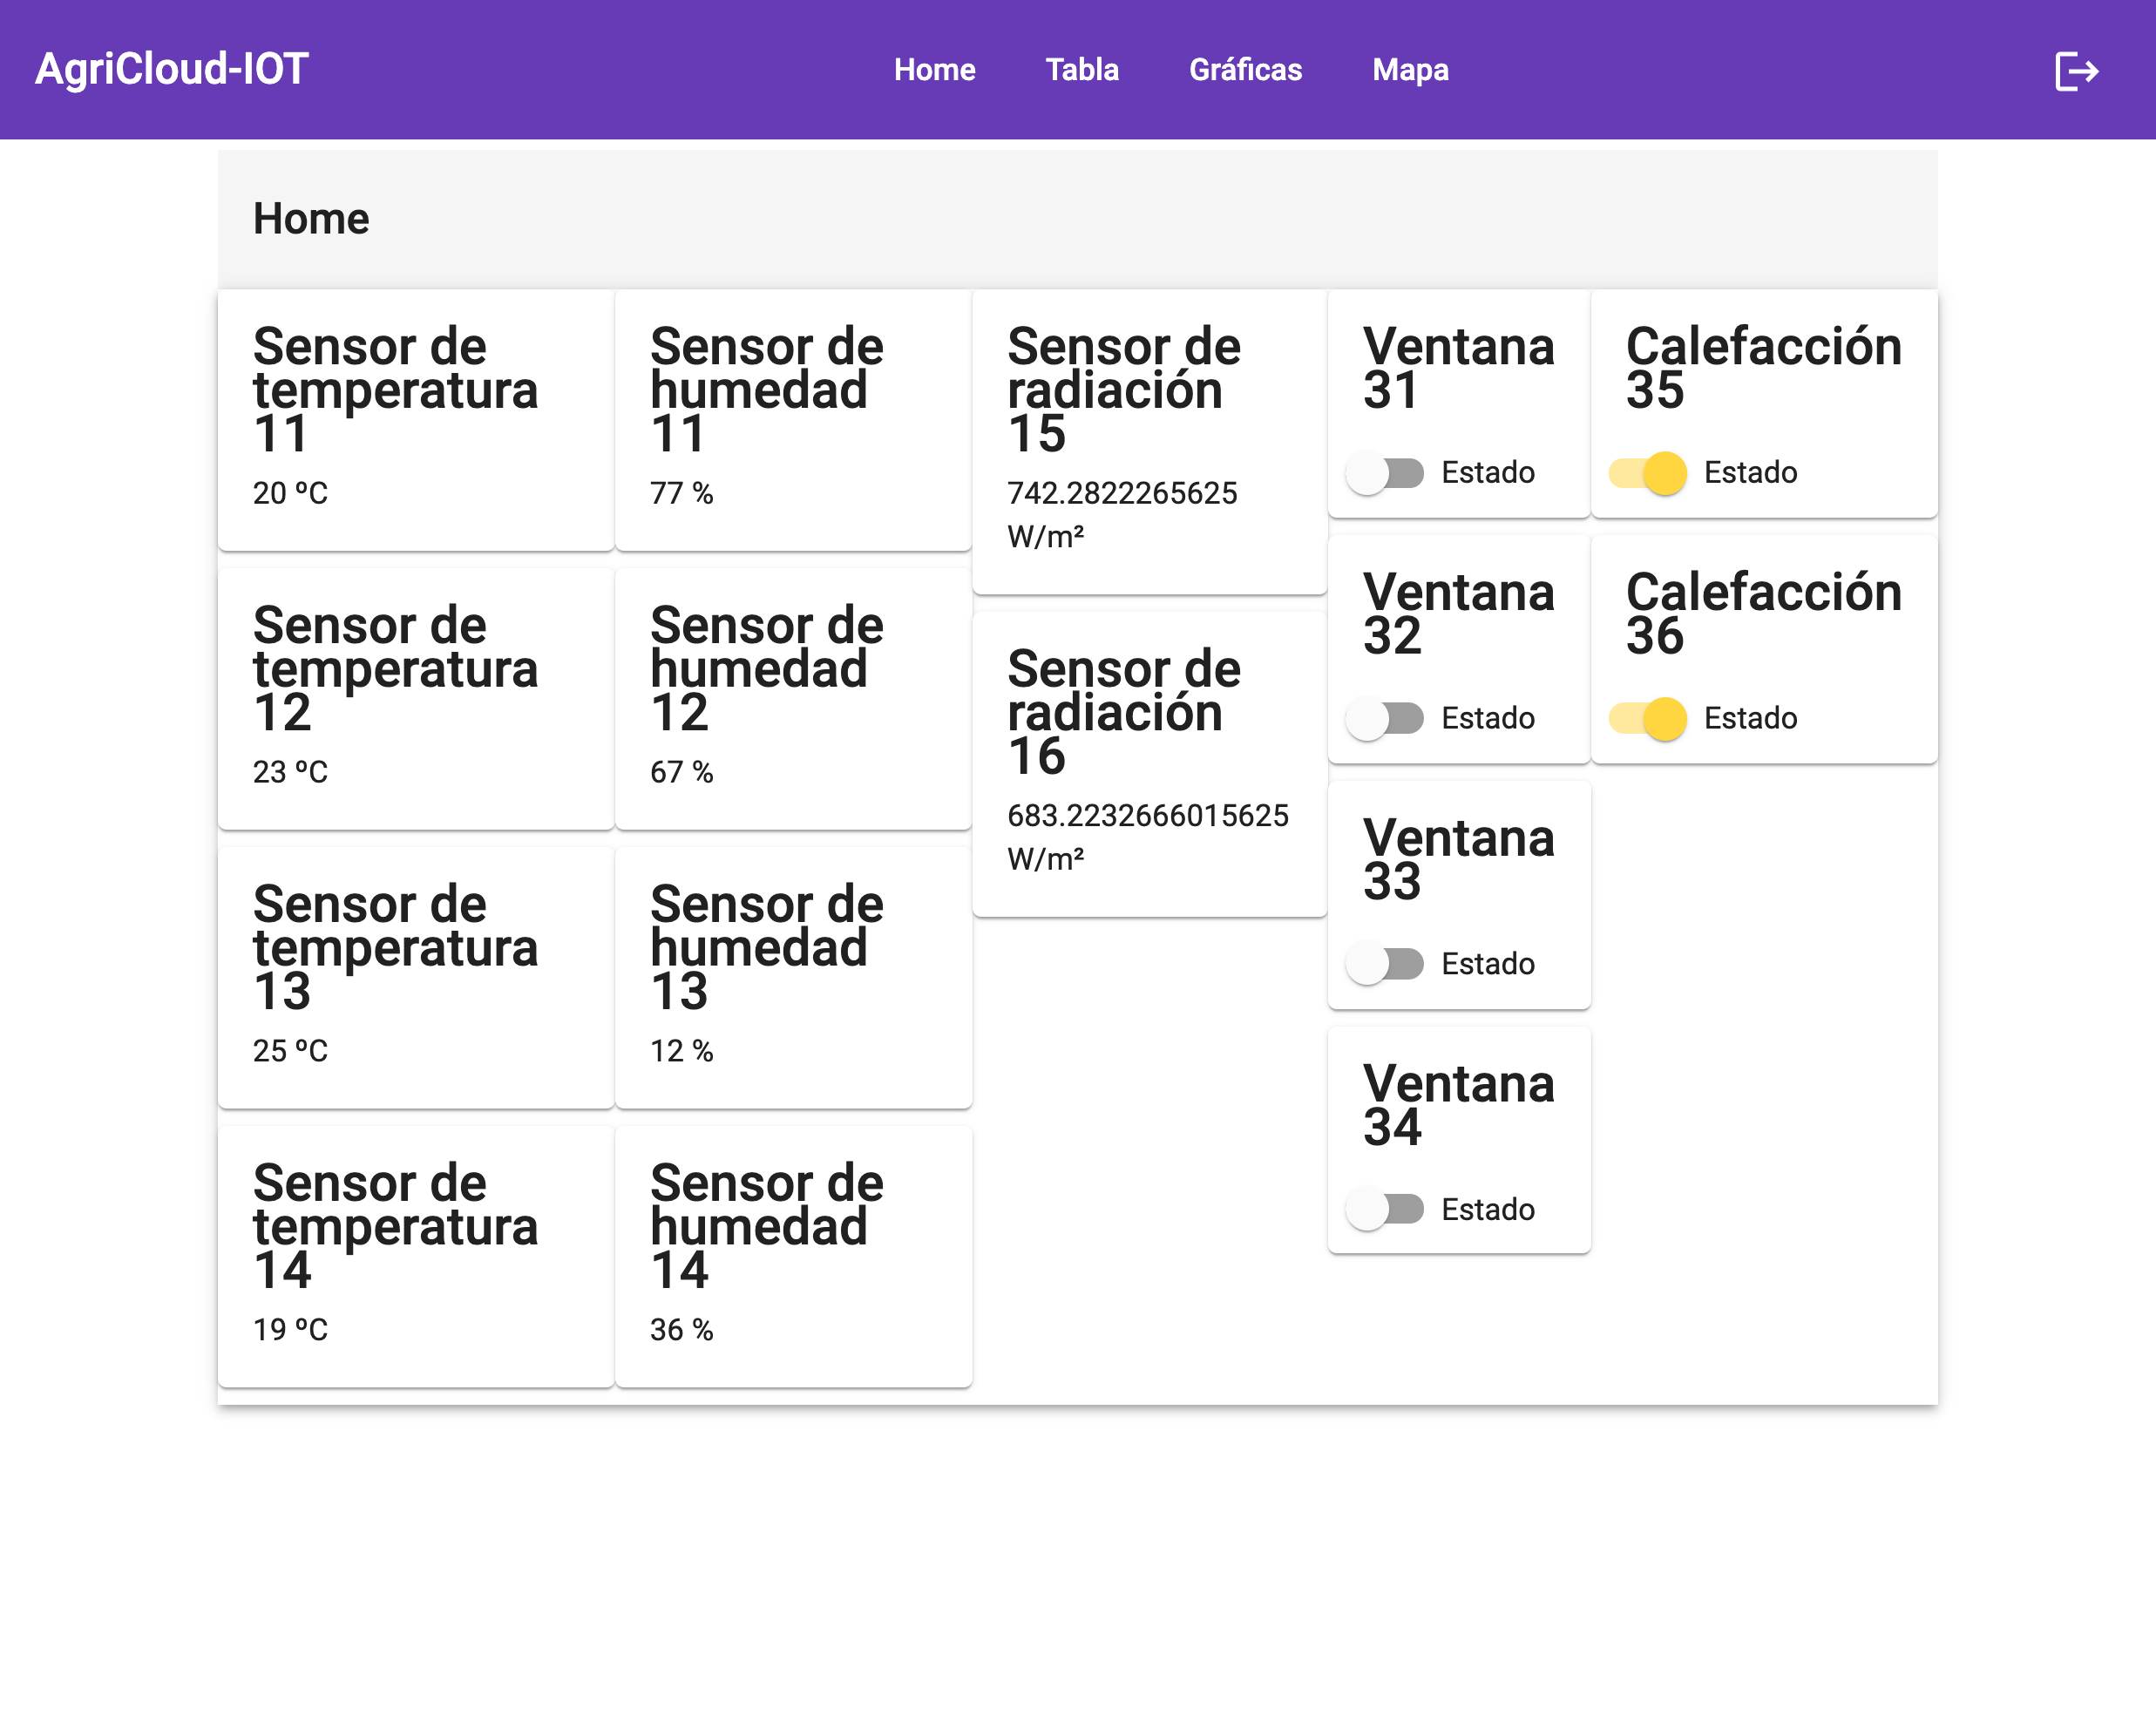
\includegraphics[width=0.8\textwidth]{img/06-Web-home.png}
    \captionof{figure}{Página principal}
    \label{fig:home-final}
\end{center}

\subsection{Tabla de datos}

Respecto a la tabla de datos, esta ha implementado paginación para una visualización más cómoda, posibilidad de ordenamiento de los datos según cada cabecera o filtrado de estos datos.

Por lo tanto, en el caso de se que quiera buscar por una hora, se escribiría en el filtro la hora, o si se quiere ordenar de mayor a menor tomando como referencia el tiempo, solo sería necesario hacer click en esa columna.

\newpage

\begin{center}
    \centering
    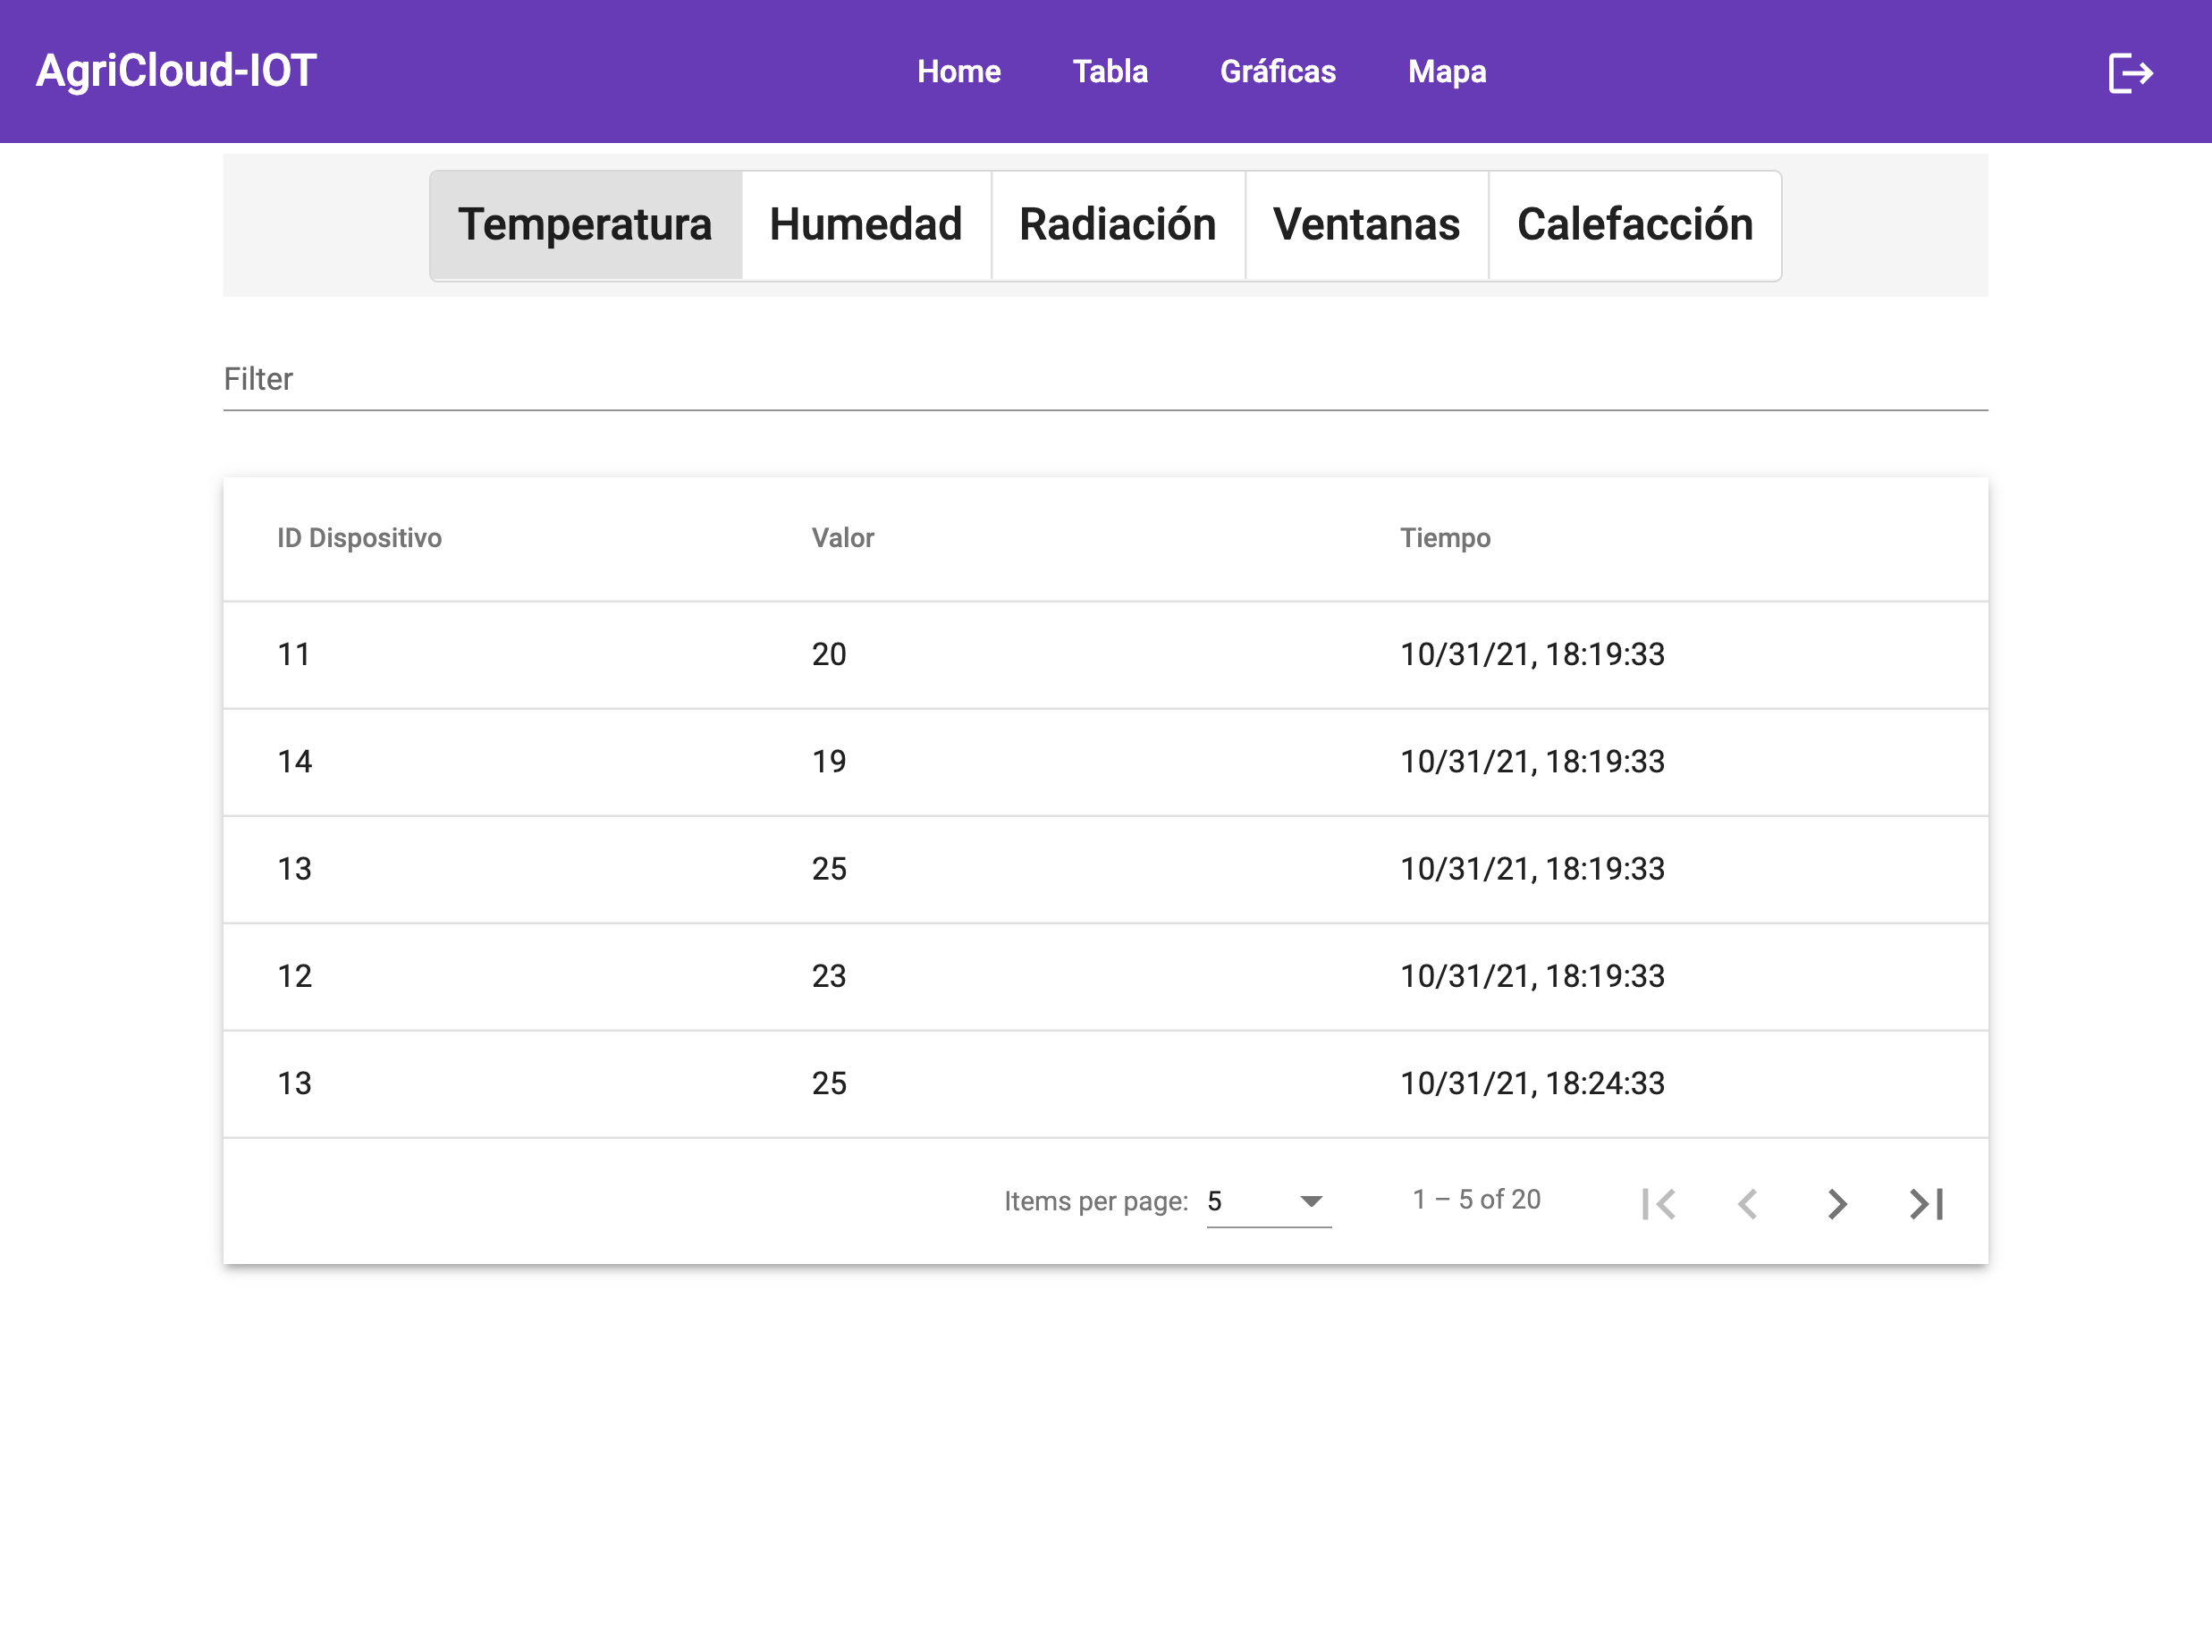
\includegraphics[width=0.8\textwidth]{img/06-Web-tablas.png}
    \captionof{figure}{Tablas de datos}
    \label{fig:tablas-de-datos-final}
\end{center}

\subsection{Gráficos}

Esta sección hace uso de Google Charts \cite{charts-google}, en concreto un paquete disponible para Angular publicado en Github.

Se han escogido las gráficas tipo lineal ya que permiten de un vistazo ver los cambios en los datos producidos en los diferentes sensores.

\begin{center}
    \centering
    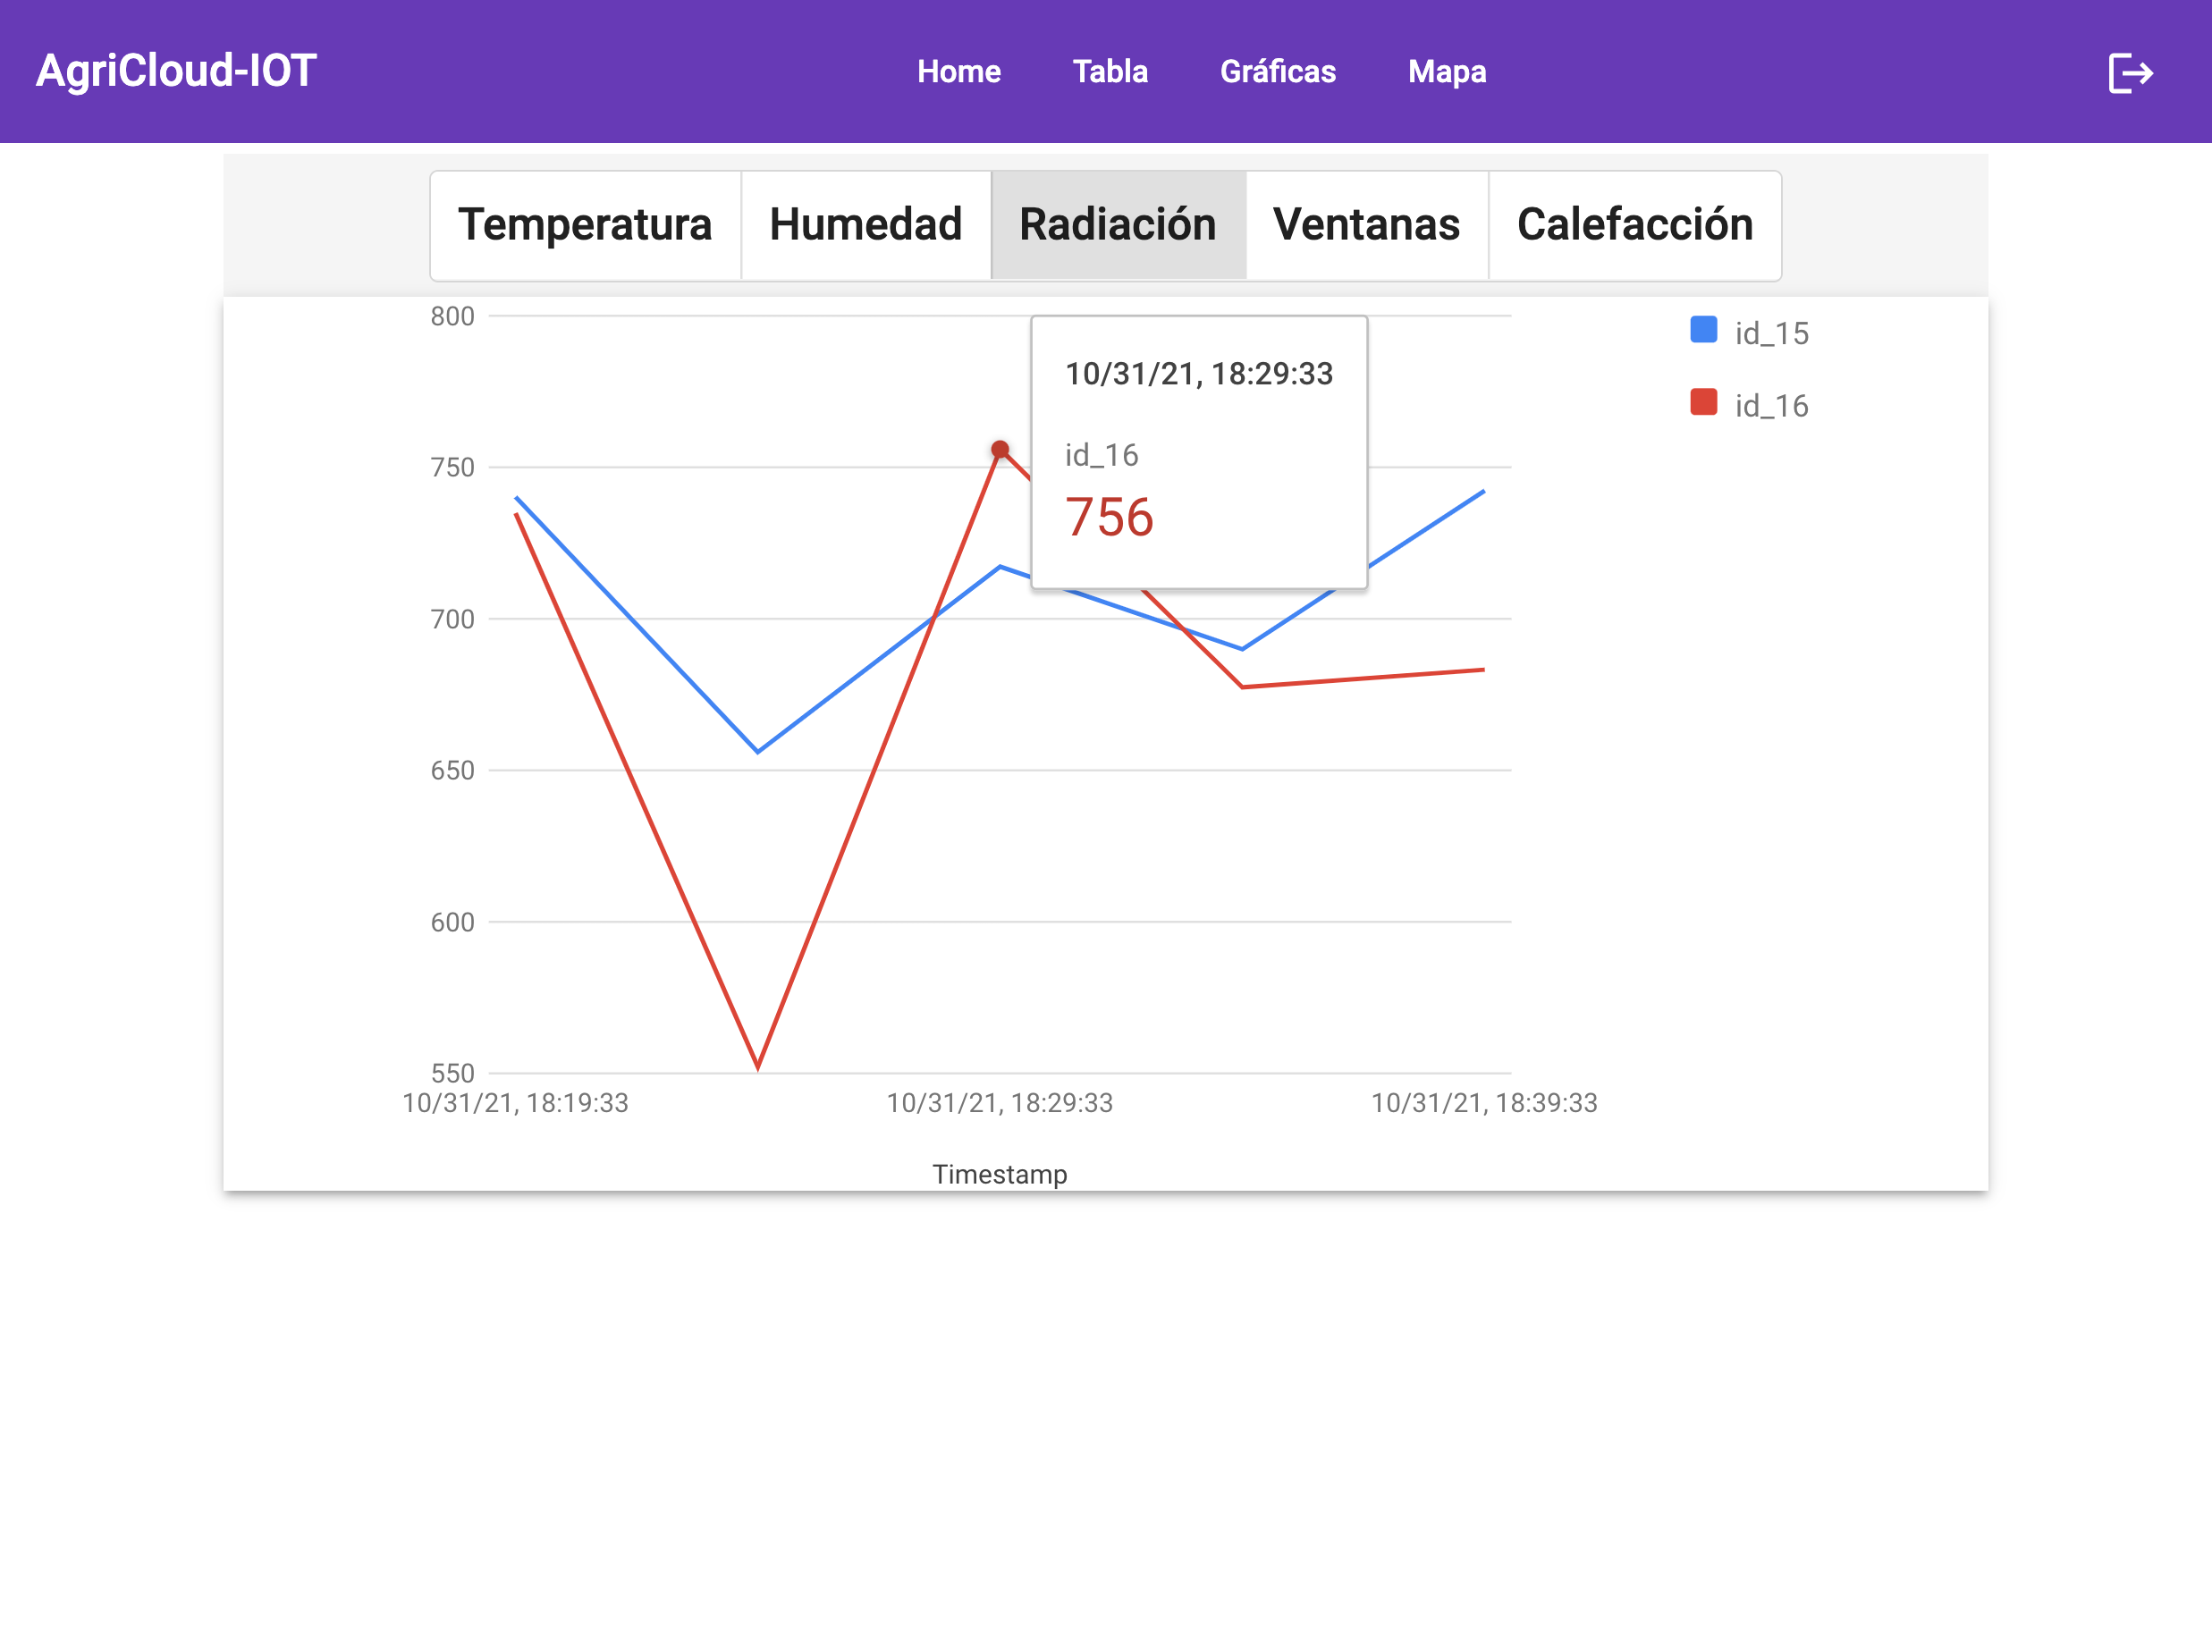
\includegraphics[width=0.8\textwidth]{img/06-Web-charts.png}
    \captionof{figure}{Gráficas de radiación}
    \label{fig:graphs-final}
\end{center}


\subsection{Mapa}

En la imagen \ref{fig:mapa-final} se muestra el mapa final, similar al mostrado en la figura del capítulo de análisis \ref{fig:mapa}, para que el usuario que acceda pueda visualizar la posición de cada nodo, además de poder obtener los datos de este al seleccionarlo, mostrados en el recuadro superior.

\begin{center}
    \centering
    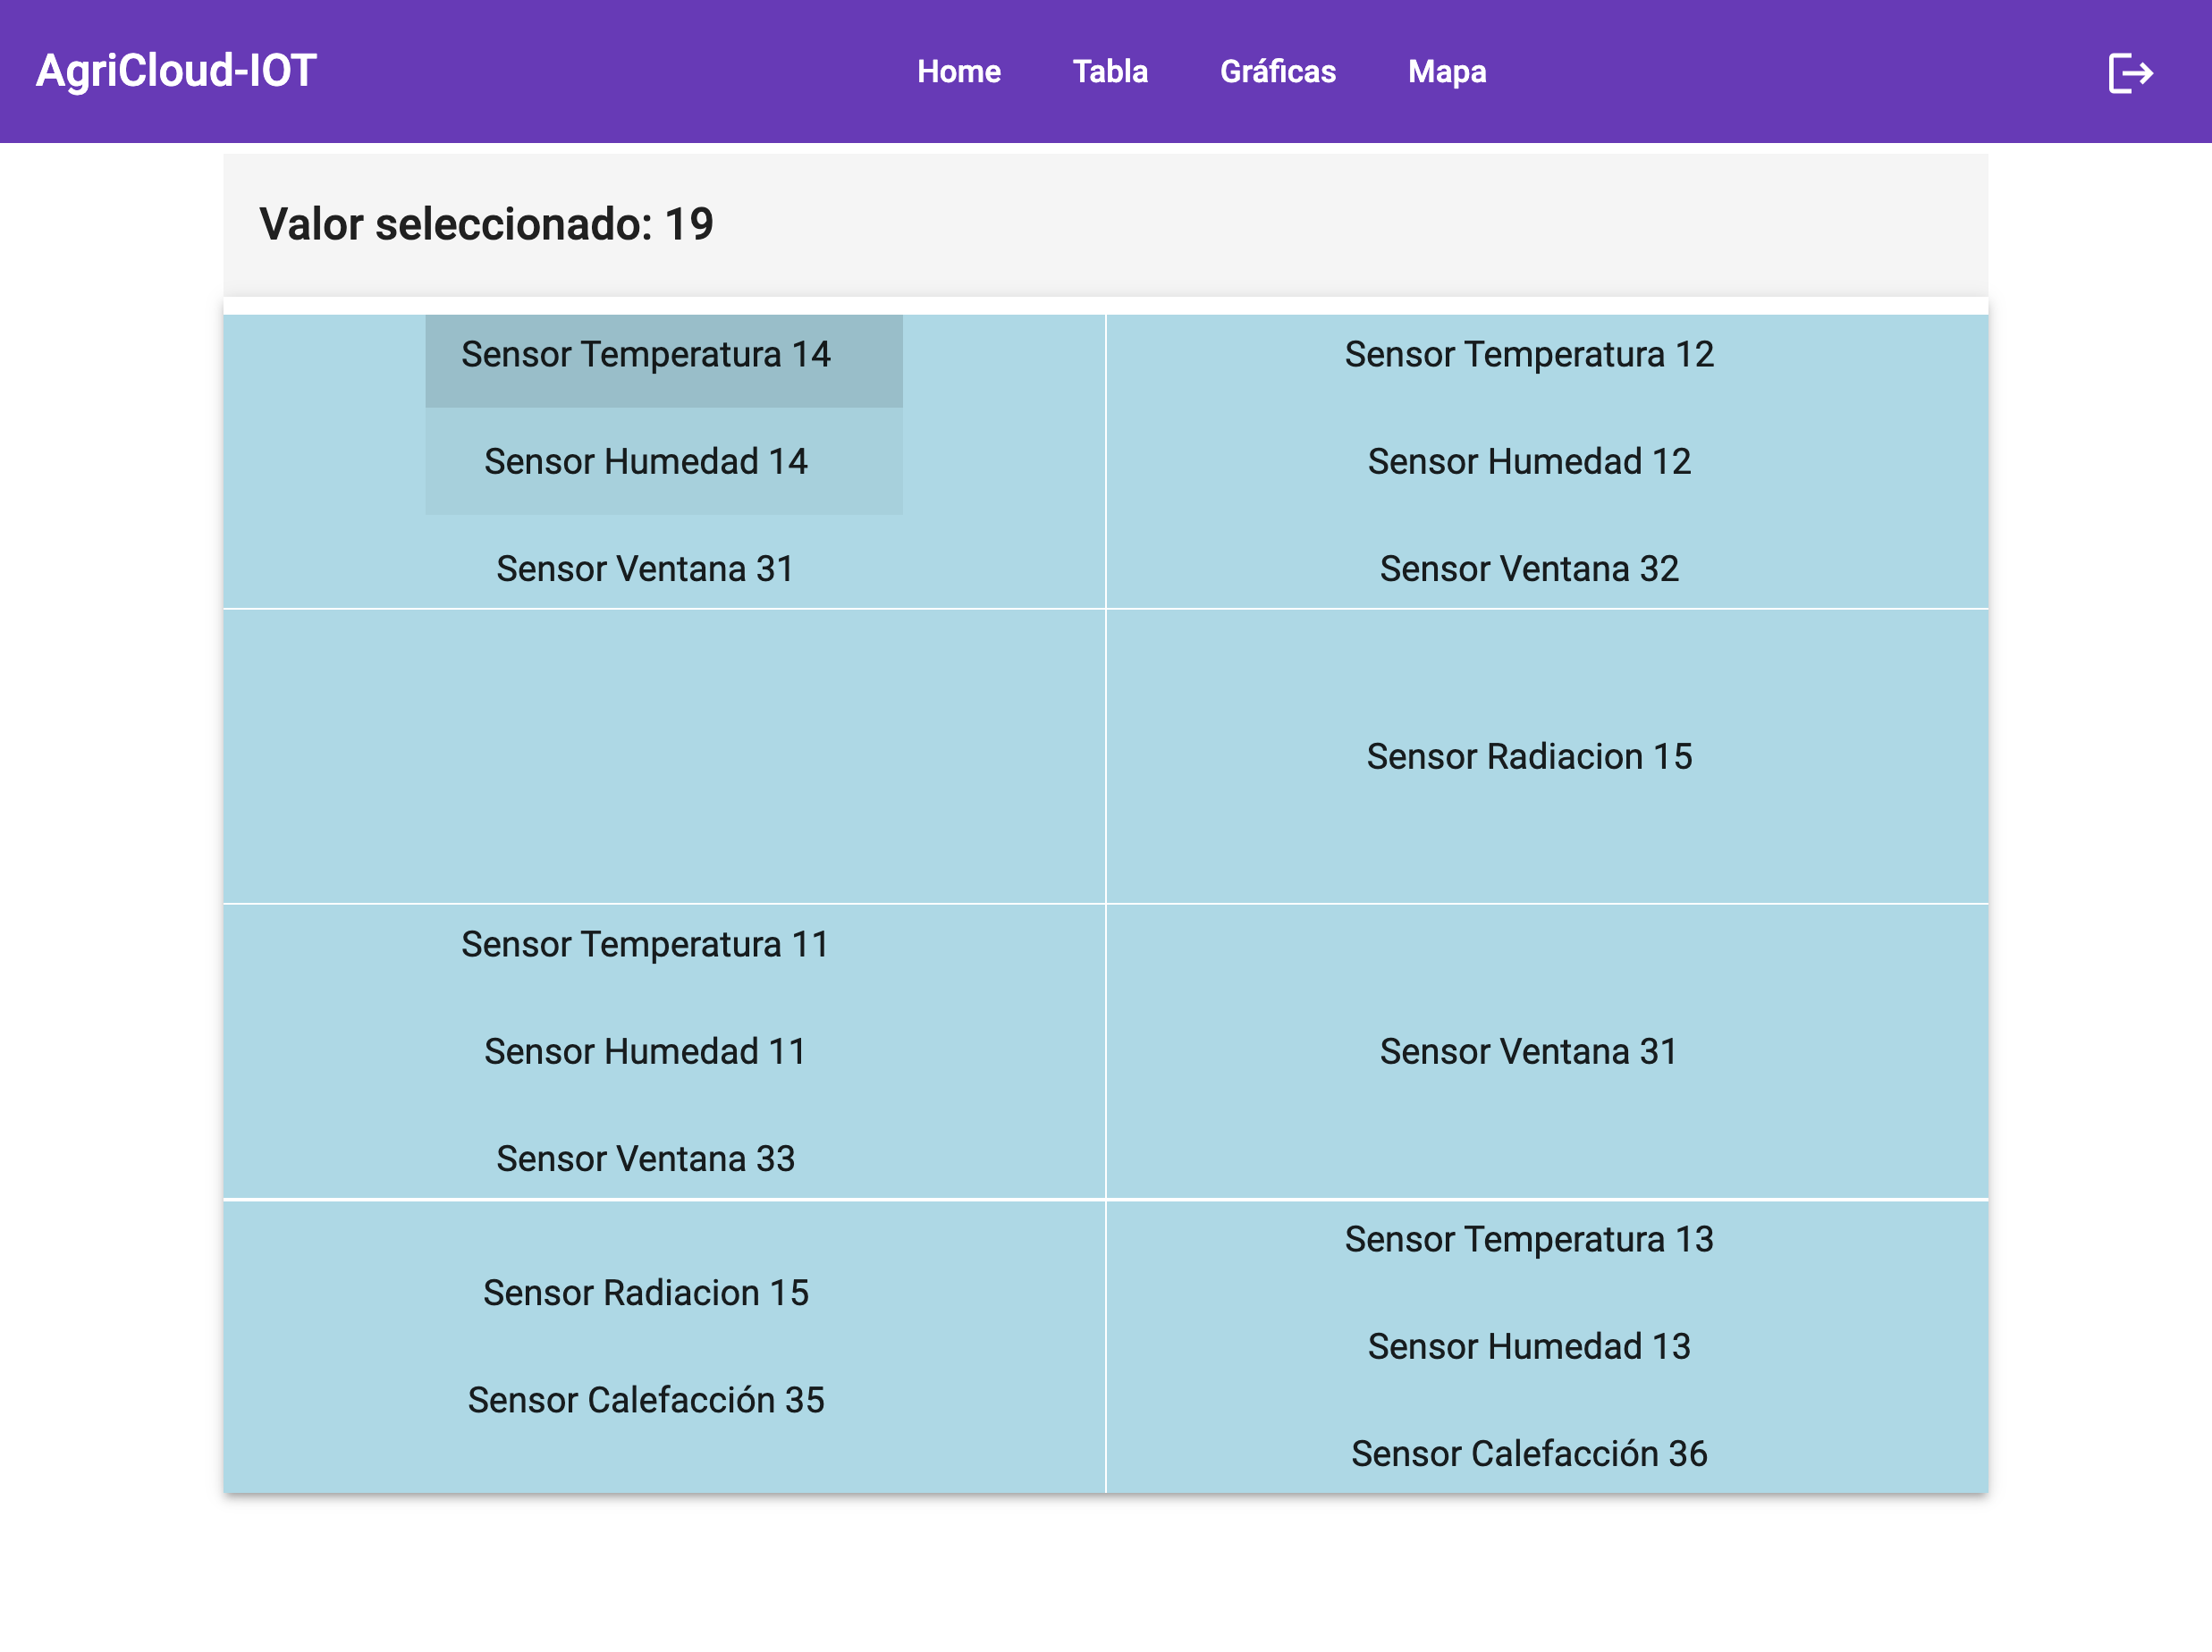
\includegraphics[width=0.8\textwidth]{img/06-Web-map.png}
    \captionof{figure}{Mapa interactivo con los diferentes sensores}
    \label{fig:mapa-final}
\end{center}

\newpage

\subsection{Login}

Se ha querido dejar hecho una página de inicio de sesión, ya que a lo largo de la implementación de la interfaz web, se ha planteado el acceso de diferentes usuarios a esta plataforma.

Por ello se muestra en la siguiente captura \ref{fig:login-final} la introducción de las credenciales de usuario.

\begin{center}
    \centering
    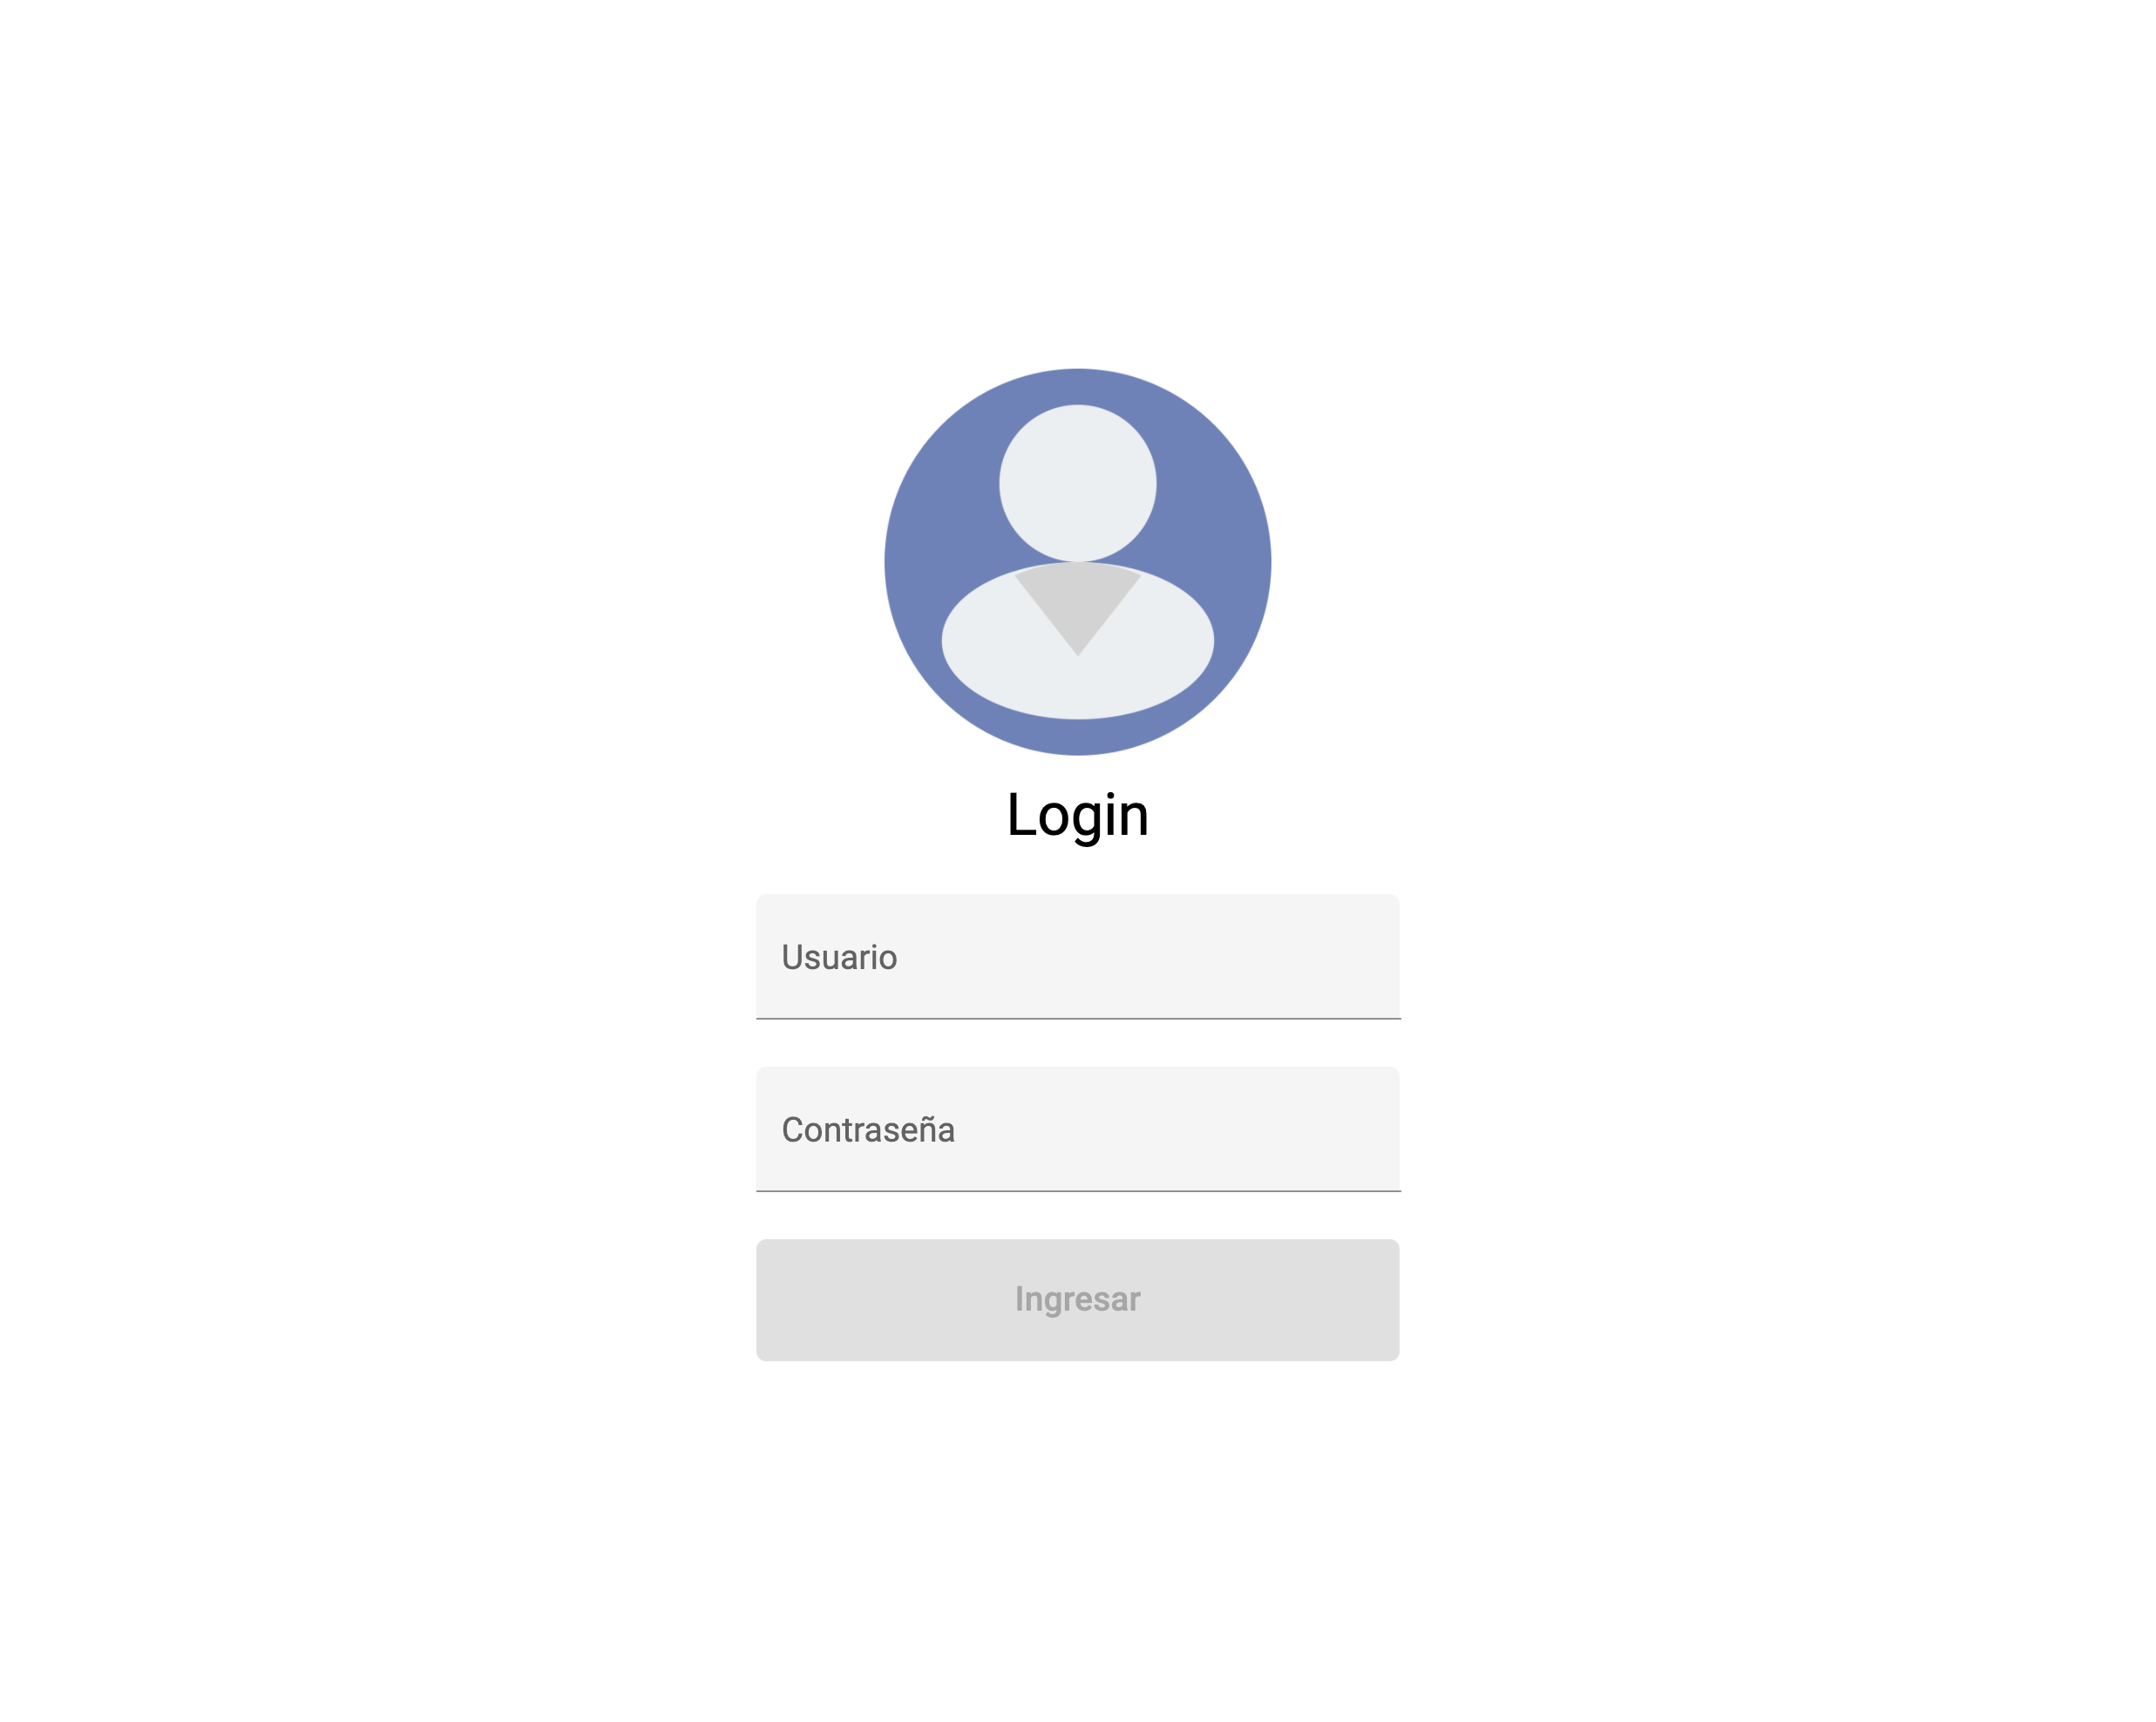
\includegraphics[width=0.8\textwidth]{img/06-Web-login.png}
    \captionof{figure}{Login implementado}
    \label{fig:login-final}
\end{center}

Esta podría ser la página principal de nuestra interfaz, y tras introducir nuestras credenciales ya se muestre el Home correspondiente a ese usuario.

	% Evaluación
	
	\chapter{Evaluación}

En este capítulo se analizará el escenario implementado con los distintos dispositivos explicados a lo largo de la documentación. El objetivo es ver si con una Raspberry Pi se puede realizar este escenario o a mayor escala.

Por recordar, los elementos utilizados son los siguientes:

\begin{itemize}
    \item Portátil Asus ROG GL752VW con un i7-6700HQ y 24GB de memoria RAM
    \item Raspberry Pi modelo 3B con 1GB de RAM
    \item 2 Microcontroladores ESP32
\end{itemize}

En la implementación, en la sección sobre el fichero de ejecución de múltiples nodos, este es ejecutado en el portátil mencionado para las diferentes pruebas. 

En este caso se va a realizar otro archivo diferente, que agrupe los nodos de \textit{Controlador}, \textit{Base de Datos} y los contenedores que actúan como agentes de microROS para recopilar y publicar la información en el dominio utilizado.

El objetivo es ver el consumo de memoria por parte de los procesos anteriores ejecutados en la Raspberry Pi.

Para ver si se producen cambios en la memoria si hay más o menos nodos en la red, estos serán ejecutados en el portátil mencionado.

\section{Escenario 1}

Se va a ejecutar un único fichero, el nodo Controlador en la Raspberry Pi, para ello se verá la memoria antes y después de la ejecución. El comando a utilizar va a ser \textit{free -h} que nos devuelve el uso de esta dividida en las diferentes cabeceras.

\begin{center}
    \centering
    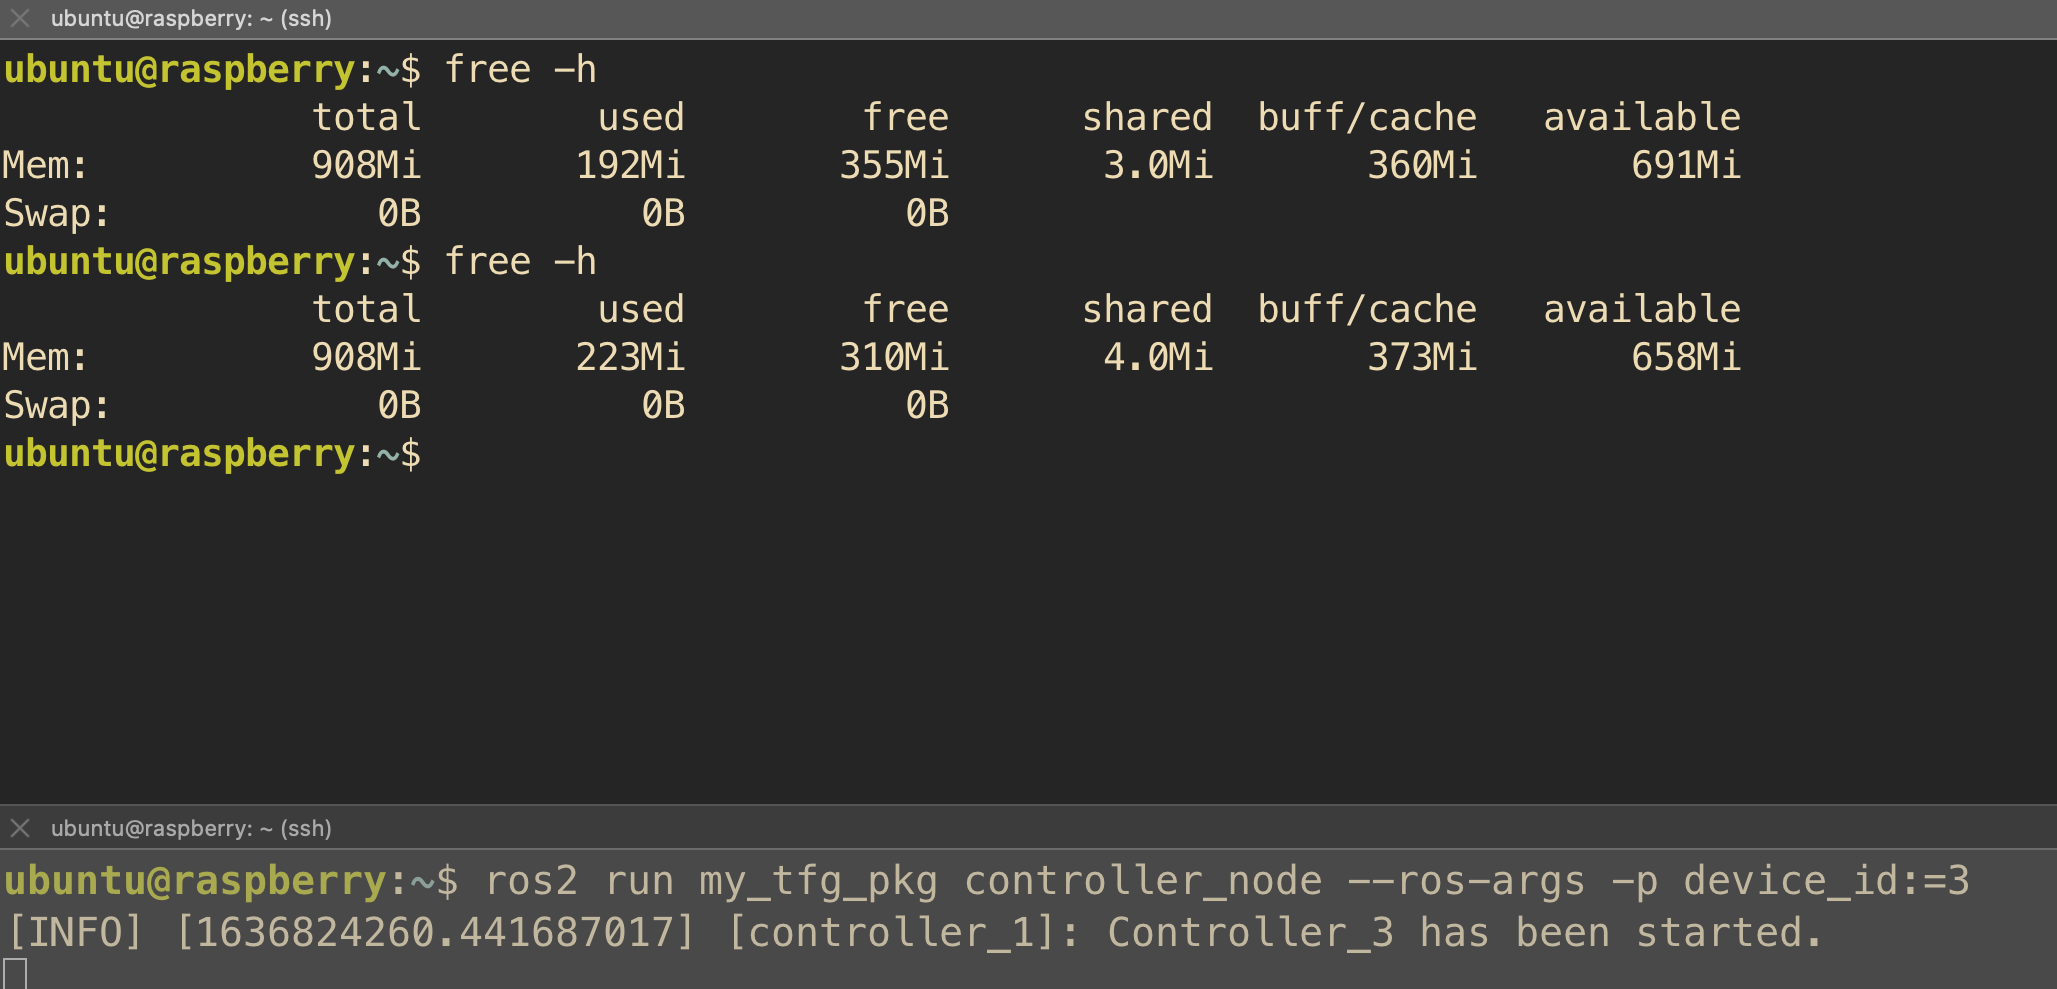
\includegraphics[width=\textwidth]{img/09-Escenario1.png}
    \captionof{figure}{Escenario 1}
    \label{fig:escenario-1}
\end{center}

En la figura \ref{fig:escenario-1} se puede observar dos ejecuciónes para medir la memoria en la parte superior, una ejecutada antes y otra después de la llamada al nodo controlador. Por tanto el consumo de memoria producido en este caso es de 41MB. 

Tras la ejecución de este escenario unas 5 veces, el consumo de memoria se ha mantenido igual, variando 1MB en algunos casos, pudiendo ser debido a otro proceso del sistema.

\section{Escenario 2}

En este caso se han lanzado diferentes nodos en la Raspberry Pi, el Controlador y el gestor de la base de datos. Al igual que en el caso anterior, se va a medir la memoria con \textit{free -h} en el mismo formato:

\newpage

\begin{center}
    \centering
    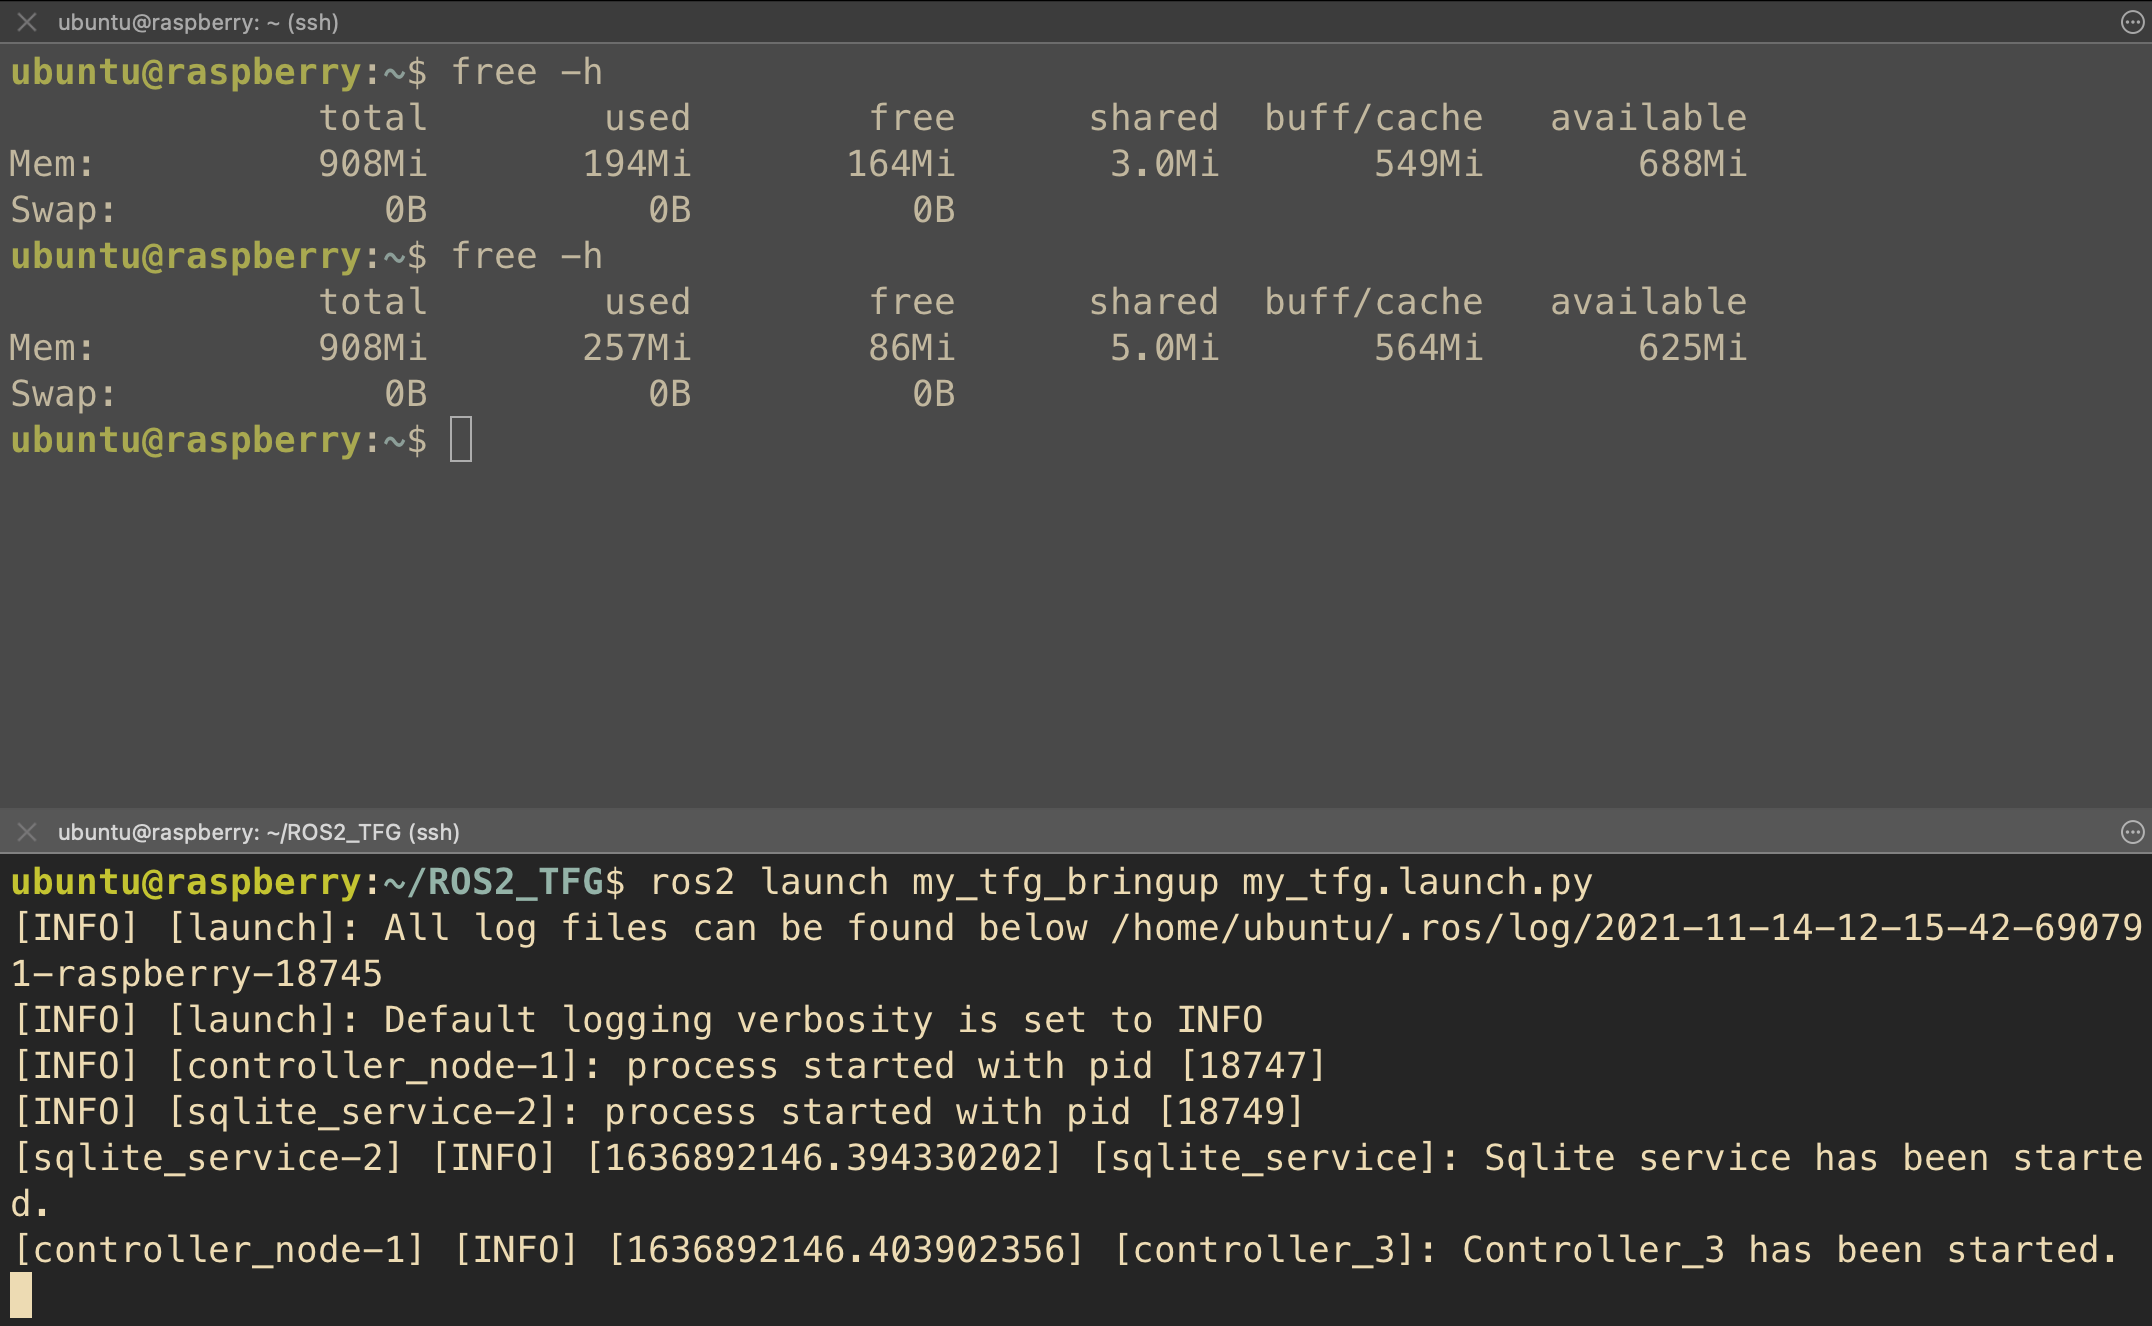
\includegraphics[width=\textwidth]{img/09-Escenario2.png}
    \captionof{figure}{Escenario 2}
    \label{fig:escenario-2}
\end{center}

Como se puede observar, el consumo de la memoria ha aumentado respecto al anterior ya que se están ejecutando actualmente dos nodos, siendo este de 63MB al ser ejecutado.

\section{Escenario 3}

Por último, se van a lanzar todos los nodos mostrados en la figura \ref{fig:rqt-graphs} en el capítulo de implementación. Además de esos, estará la Raspberry Pi 3B con los nodos en ejecución, para ver si se refleja toda la comunicación en la memoria. Esta parte será la mostrada en la terminal, ya que es la memoria que se está analizando.

\newpage

\begin{center}
    \centering
    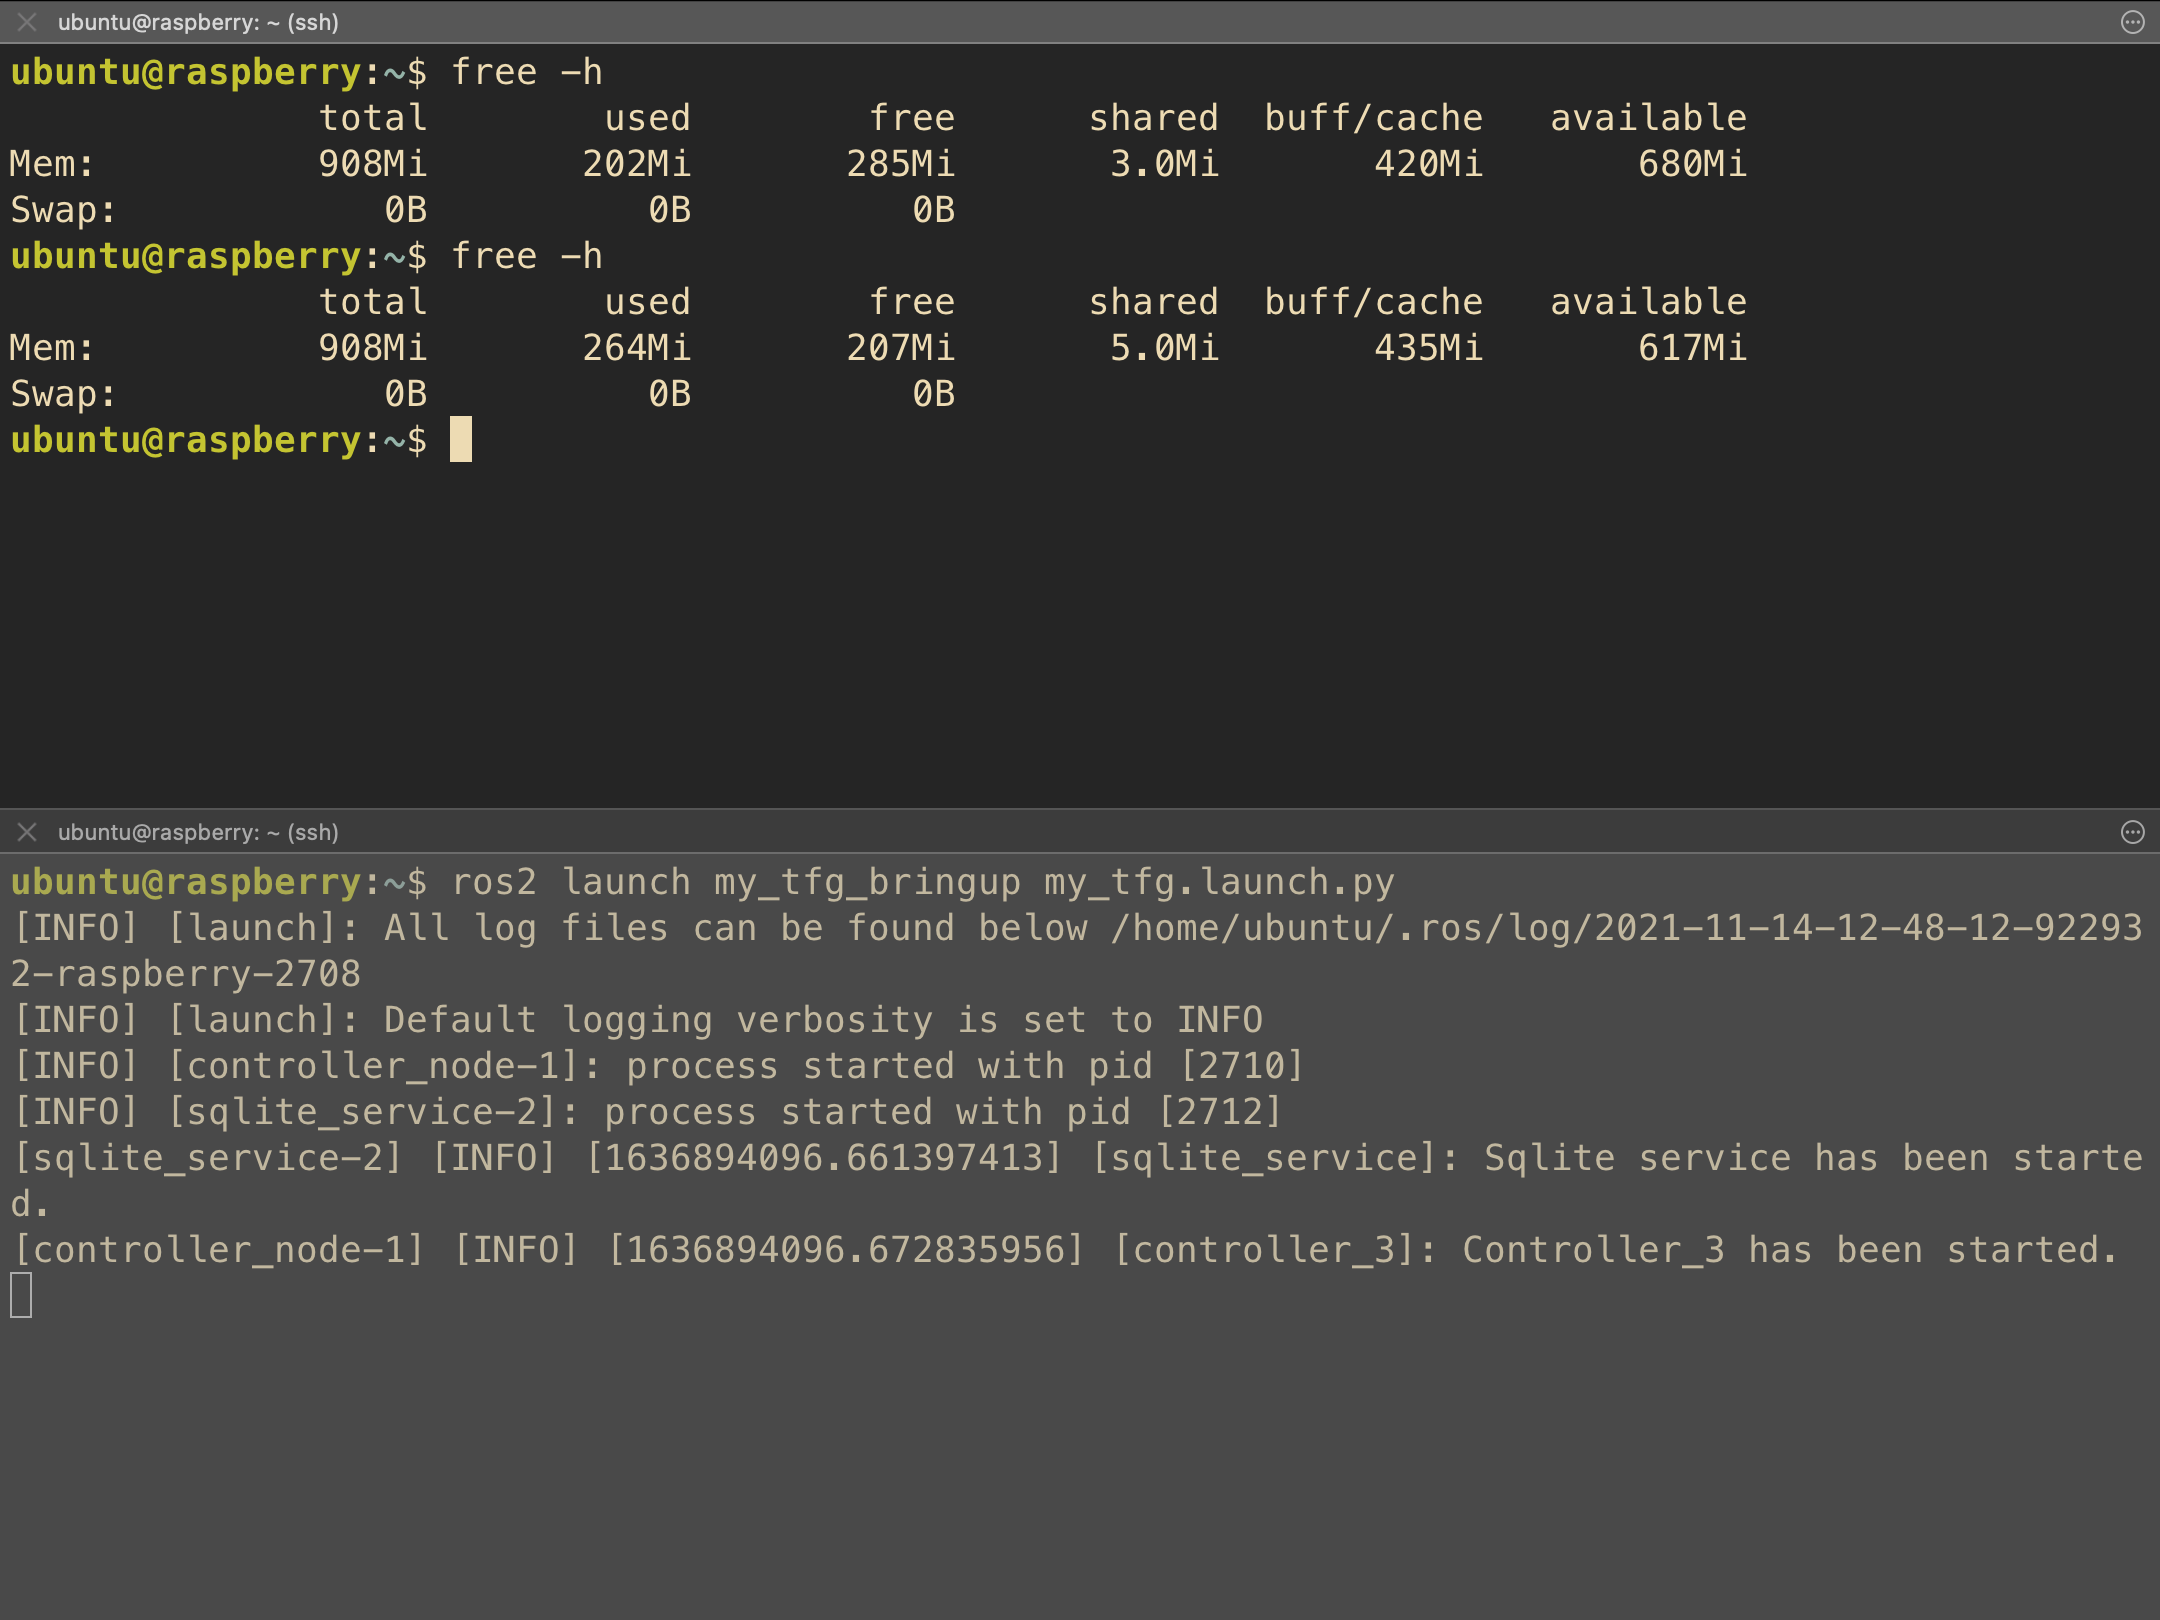
\includegraphics[width=\textwidth]{img/09-Escenario3.png}
    \captionof{figure}{Escenario 3}
    \label{fig:escenario-3}
\end{center}

Al igual que en el escenario 2, el consumo de memoria mostrado en la figura \ref{fig:escenario-3} es de 63MB.

Por comprobar esta variación, se ha ejecutado este escenario 5 veces, obteniendo los casi mismos resultados en las diferentes ocasiones, mostrado en la siguiente tabla:


\begin{center}
\begin{tabular}{||c c c c||} 
 \hline
  & Memoria Inicial & Memoria en ejecución & Memoria consumida \\ [0.5ex] 
 \hline\hline
 1 & 680 & 617 & 63 \\ 
 \hline
 2 & 685 & 623 & 62 \\
 \hline
 3 & 686 & 623 & 63 \\
 \hline
 4 & 685 & 623 & 62 \\ 
 \hline
 5 & 685 & 623 & 62 \\


 \hline
\end{tabular}
\captionof{figure}{Tabla de Temperatura}
\end{center}

Para poder analizar el estado de la red de los diferentes nodos, se va a mostrar un gráfico utilizando el programa rqt\_graph.

\begin{center}
    \centering
    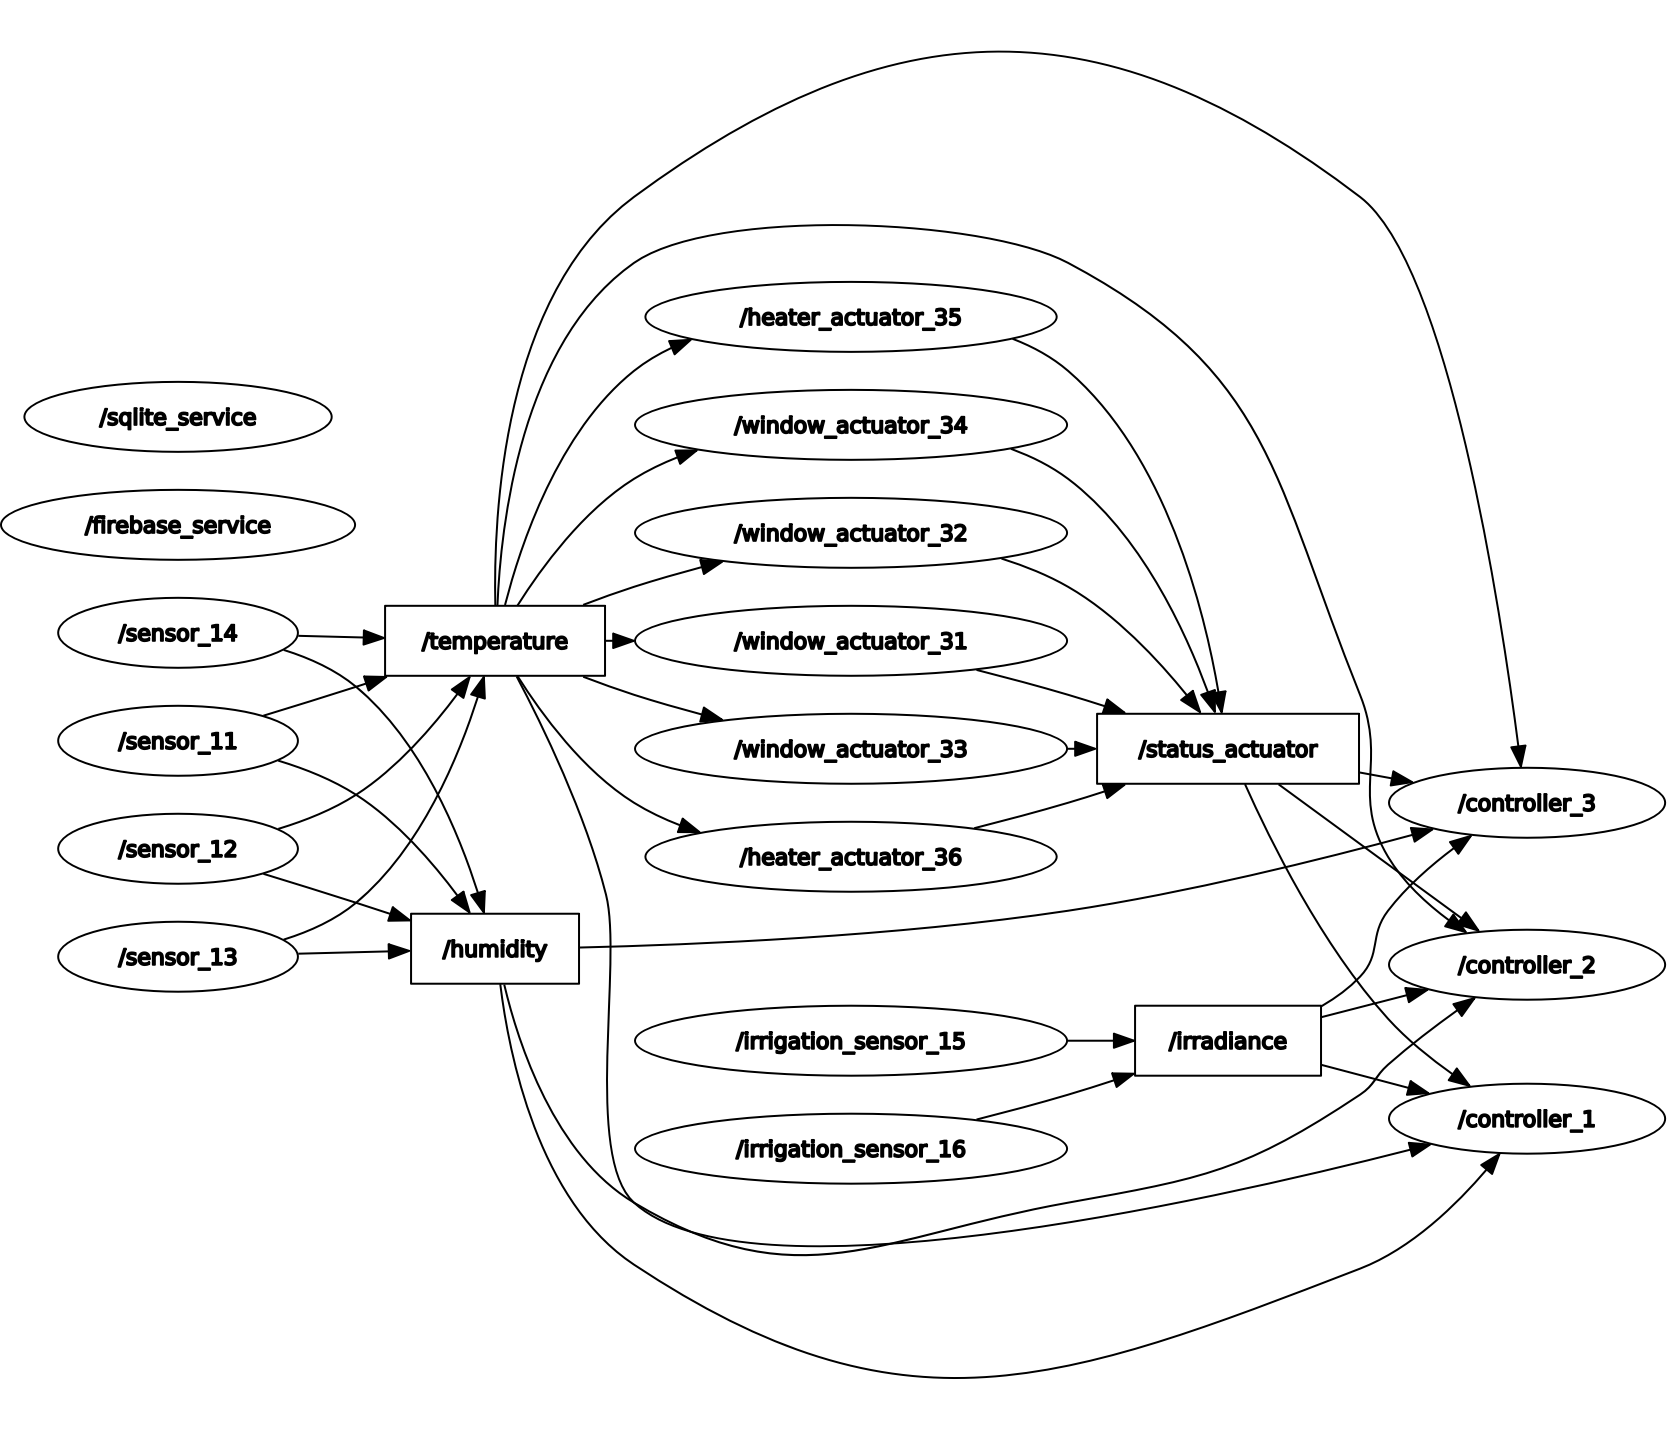
\includegraphics[width=\textwidth]{img/09-Escenario-3-rosgraph.png}
    \captionof{figure}{Red en el Escenario 3}
    \label{fig:rqt-escenario-3}
\end{center}

Por aclarar este escenario, al igual que se ha explicado en el diagrama del análisis \ref{fig:diagrama-comunicacion-nodos} y en la implementación \ref{fig:rqt-graphs}, los rectángulos representan los tópicos y los óvalos representan los diferentes nodos.

Para especificar donde se estaba ejecutando cada nodo, se va a listar a continuación:

\begin{itemize}
    \item Las placas ESP32 están representadas con \textbf{sensor\_11} y \textbf{sensor\_12}
    \item La Raspberry Pi 3B utilizada durante todo el escenario está ejecutando los nodos \textbf{controller\_3} y \textbf{sqlite\_service}
    \item El portátil Asus esta ejecutando los demás dispositivos de manera virtual.
\end{itemize}

Finalizando esta sección, se ha utilizado Wireshark \cite{wireshark} para capturar el tráfico generado en la red. 

Tras dejar el sistema durante 30 minutos en ejecución, se ha aplicado como filtro que el protocolo utilizado sea RTPS, ya que es utilizado en la comunicación entre los diferentes nodos.

Con la funcionalidad de Stadistics ofrecida por Wireshark, se ha obtenido una gráfica mostrando la cantidad de paquetes cada 10 segundos, representado en la siguiente imagen:

\begin{center}
    \centering
    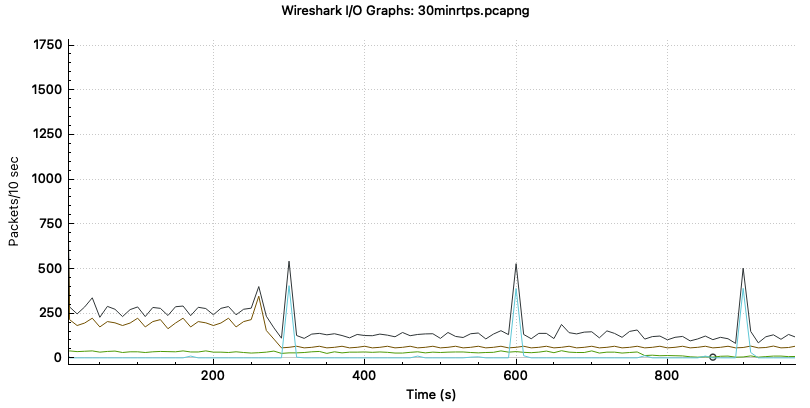
\includegraphics[width=\textwidth]{img/09-30minrtps.png}
    \captionof{figure}{Gráfica generada por Wireshark}
    \label{fig:wireshark-30min}
\end{center}

Como se puede observar, hay varias líneas mostradas en el gráfico:

\begin{itemize}
    \item La marrón es el protocolo RTPS
    \item La verde es el protocolo ARP
    \item La azul es el protocolo TCP
    \item La negra es el número de paquetes total
\end{itemize}

Cada cierto tiempo, se produce un pico de paquetes en la red se vuelve a estabilidad. Esto es debido al almacenamiento de los datos en la plataforma de Firebase, que se ejecuta cada ese periodo, establecido con un temporizador.

Por lo tanto se podría concluir que la cantidad de paquetes es estable respecto a RTPS una vez pasado un tiempo desde que comienza la red, y la comunicación con la base de datos cada este periodo produce esos picos.

	% Conclusiones
	\chapter{Conclusiones y trabajo futuro}

En este trabajo se han conseguido cumplir los tres objetivos principales propuestos en la introducción. Entre ellos destacar la posibilidad de añadir diferentes nodos al sistema sin tener que realizar modificaciones o solo las mínima. Esto ha sido posible gracias al haber hecho uso de ROS 2 junto al paradigma Publicador-Suscriptor, únicamente teniendo que definir un publicador o suscriptor nuevo relacionado con los tópicos existentes en esta red.

Tras el estudio de algunas de las herramientas ofrecidas por ROS 2, se han analizado todas las funcionalidades que nos otorga. Además se han aprendido diferentes conceptos relacionados con esta tecnología utilizada en más escenarios de los que se pensaba al principio, y la potencia que tiene al utilizarse en el ámbito de IoT.

Respecto a la interfaz se han podido comprender las bases del funcionamiento del Angular y la estructura de un proyecto de este tipo, diferenciando componentes, módulos y derivados.

Además, gracias a las evaluaciones de los diferentes escenarios, se ha llegado a la conclusión que la Raspberry Pi3B es más que solvente para la ejecución de los nodos requeridos, sin ver influencias claras respecto a los datos publicado en la red producidos por los demás nodos.

Para comentar las tareas que han quedado por realizar se pueden leer en la siguiente sección.

\section{Trabajo futuro}

Debido al uso de diferentes tecnologías de las cuales se desconocían su funcionamiento y como trabajar con ellas, tras un periodo de estudio y asimilación de conceptos se ha podido lograr el trabajo anterior. Pero hay puntos por realizar, que en el caso de algunos de ellos, si se hubiese querido implementar todas sus funcionalidades, probablemente daría para otro documento de similar extensión a este.

\begin{itemize}
    \item \textbf{Capa de Seguridad.} Es necesario encriptar la información y la gestión de los diferentes usuarios en el sistema, añadiendo las tablas que sean necesarias en la base de datos.
    \item \textbf{Extensión de la API REST.} Esta tarea tiene mucho potencial para futura interacción con el sistema, pudiendo acceder a estos datos para ser tratados con distintos fines.
    \item \textbf{Test de carga y despliegue de los dispositivos en un entorno real.} Para ello es necesario un estudio con personal con más conocimientos sobre los diferentes sensores en el mercado y que sería de necesidad en estos escenarios.
\end{itemize}

        
	
	\newpage
	\bibliography{bibliografia}
	\bibliographystyle{plain}
	
	% Trabajos futuros
    \chapter*{Acrónimos}
\begin{acronym}[STOMP] % Give the longest label here so that the list is nicely aligned
\acro{AMQP}{Advanced Message Queuing Protocol}
\acro{APIs}{Application Programming Interfaces}
\acro{ASGI}{Asynchronous Server Gateway Interface}
\acro{DDS}{Data Distribution Service}
\acro{FreeRTOS}{Real-time operating system for microcontrollers}
\acro{GPRS}{Servicio General de Paquetes vía Radio}
\acro{IA}{Inteligencia Artificial}
\acro{IDL}{Interface Description Language}
\acro{IoT}{Internet of the Things}
\acro{ISS}{International Space Station}
\acro{MIT}{Massachusetts Institute of Technology}
\acro{MoM}{Message-oriented Middleware}
\acro{MQTT}{MQ Telemetry Transport}
\acro{OMG}{Object Management Group}
\acro{QoS}{Quality of Service}
\acro{REST}{REpresentational State Transfer}
\acro{ROS}{Robot Operating System}
\acro{STOMP}{Streaming Text Oriented Messaging Protocol}
\acro{TICs}{Tecnologías de Información y Comunicación}
\end{acronym}
    \addcontentsline{toc}{chapter}{Acónimos}
	
\end{document}

